\documentclass[12pt,twoside,onecolumn]{book}
\usepackage[a4paper,top=2.5cm,bottom=2.5cm,left=3cm,right=2.5cm]{geometry}
\usepackage[absolute]{textpos}
\setlength{\TPHorizModule}{10mm}
\setlength{\TPVertModule}{\TPHorizModule}
\textblockorigin{0mm}{0mm}

% croatian words break
\usepackage[english]{babel}

% for hacking
\usepackage{xpatch}
\newenvironment{block}%
  {\list{}{\leftmargin=0.0in\rightmargin=0.0in}  \item[]  }%
  {\endlist}

% fonts
\usepackage[utf8]{inputenc}
\usepackage[T1]{fontenc}

% appendix setup
\usepackage[titletoc,title]{appendix}

% not-so-intelligent cross-referencing
\usepackage[linktocpage=true]{hyperref}

% additional stuff for "description" lists
\usepackage{calc}  
\usepackage{enumitem}

% embed pdfs into latex
% \usepackage[draft]{pdfpages}
\usepackage{pdfpages}

% remove headers/footers for empty pages
\usepackage{emptypage}

% math packages
\usepackage{amsmath, amsfonts, amssymb}
\usepackage{bm}
\usepackage{nicefrac}

% SI units in text
\usepackage[detect-all]{siunitx}
\sisetup{per-mode=symbol,range-phrase=--,range-units=single,list-units=single}
\usepackage{booktabs}

% tables
\usepackage{rotating}
\usepackage{tabularx}
\usepackage{multirow}
\usepackage{makecell}
%\usepackage[table,xcdraw]{xcolor}  % needs to be loaded before pgf

% figures
\usepackage{tikz}
\usetikzlibrary{calc,positioning,shapes,backgrounds,fit,arrows}
\usepackage{pgf-spectra}
\usepackage{contour}
\usepackage{adjustbox}
\usepackage{wrapfig}
\def\checkmark{\tikz\fill[scale=0.4](0,.35) -- (.25,0) -- (1,.7) -- (.25,.15) -- cycle;}
\usepackage{caption}
\usepackage{subcaption}

% intelligent cross-referencing 
\usepackage{cleveref}
\xapptocmd\appendices{%
  \crefalias{chapter}{appendix}%
}{}{\PatchFailed}

% glossaries
\usepackage[acronym,nonumberlist]{glossaries-prefix}
\renewcommand*{\glstextformat}[1]{\textcolor{black}{#1}}
\makeglossaries
\newacronym{1-d}{1-D}{one-dimensional}
\newacronym{2-d}{2-D}{two-dimensional}
\newacronym{3-d}{3-D}{three-dimensional}
\newacronym{k-d}{$k$-D}{$k$-dimensional}
\newacronym{em}{EM}{electromagnetic}
\newacronym{emf}{EMF}{electromagnetic field}
\newacronym{rf}{RF}{radio frequency}
\newacronym{lf}{LF}{low frequency}
\newacronym{ir}{IR}{infrared}
\newacronym{uv}{UV}{ultraviolet}
\newacronym{mmw}{MMW}{millimeter wave}
\newacronym{5g}{5G}{fifth generation}
\newacronym{mimo}{MIMO}{multiple-input and multiple-output}
\newacronym{br}{BR}{basic restriction}
\newacronym{drl}{DRL}{dosimetric reference limit}
\newacronym{rl}{RL}{reference level}
\newacronym{erl}{ERL}{exposure reference level}
\newacronym{sar}{SAR}{specific absorption rate}
\newacronym{ipd}{IPD}{incident power density}
\newacronym{tpd}{TPD}{transmitted power density}
\newacronym{apd}{APD}{absorbed/epithelial power density}
\newacronym{icnirp}{ICNIRP}{International Commission on Non-Ionizing Radiation Protection}
\newacronym{ieee}{IEEE}{Institute of Electrical and Electronics Engineers}
\newacronym{ices}{ICES}{International Committee on Electromagnetic Safety}
\newacronym{pca}{PCA}{principal component analysis}
\newacronym{fdtd}{FDTD}{finite-difference time-domain}
\newacronym{fem}{FEM}{finite element method}
\newacronym{rms}{RMS}{root mean square}
\newacronym{rgb}{RGB}{red-green-blue}
\glsaddall

% official FESB setup and formatting - DO NOT CHANGE
\definecolor{cite}{rgb}{0,0,0.8}
\definecolor{link}{rgb}{0,0,0.8}
\hypersetup{%
    colorlinks=true,
    linkcolor=link,
    citecolor=cite,
    urlcolor=link,
    colorlinks=true,
    }%
\usepackage{setspace}
\usepackage[nottoc,notlot,notlof]{tocbibind}
\usepackage[all]{hypcap}
\usepackage{bookmark}
\usepackage{hypdestopt}
\usepackage{pslatex}
\usepackage{fancyhdr}
\usepackage{etoolbox}
\newcounter{citenum}
\def\oldcite{}
\let\oldcite=\bibcite
\def\bibcite{\stepcounter{citenum}\oldcite}

\newcounter{totfigures}
\newcounter{tottables}
\newcounter{totequations}

\makeatletter
\AtEndDocument{
    \addtocounter{totfigures}{\value{figure}}
    \addtocounter{tottables}{\value{table}}
    \addtocounter{totequations}{\value{equation}}
    \immediate\write\@mainaux{%
        \string\gdef\string\totfig{\number\value{totfigures}}
        \string\gdef\string\tottab{\number \value{tottables}}
        \string\gdef\string\toteq{\number \value{totequations}}
        \string\gdef\string\totcite{\number\value{citenum}}
    }%
}%
\makeatother
\pretocmd{\chapter}{\addtocounter{totfigures}{\value{figure}}\setcounter{figure}{0}}{}{}
\pretocmd{\chapter}{\addtocounter{tottables}{\value{table}}\setcounter{table}{0}}{}{}
\pretocmd{\chapter}{\addtocounter{totequations}{\value{equation}}\setcounter{equation}{0}}{}{}
\usepackage[T1]{fontenc}
\usepackage{titlesec}
\usepackage[nottoc,notlot,notlof]{tocbibind}

\titleformat{\chapter}
    [block]{\normalfont\bfseries\Large}{\rlap{\thechapter}}{0em}
    {\hspace*{.05\textwidth}\begin{minipage}[t]{.9\textwidth}\raggedright}[\end{minipage}]

\titleformat{\section}{\normalfont\Large\bfseries}{\thesection}{1em}{}
\titleformat{\subsection}{\normalfont\large\bfseries}{\thesubsection}{1em}{}
\titleformat{\subsubsection}{\normalfont\normalsize\bfseries}{\thesubsubsection}{1em}{}
\raggedbottom
\onehalfspacing
\makeindex%
\usepackage{tocloft}
\renewcommand\cftloftitlefont{\LARGE\bfseries}
\renewcommand\cftfigfont{\em}
\renewcommand\cftlottitlefont{\LARGE\bfseries}
\renewcommand\cfttabfont{\em}
\renewcommand\cfttoctitlefont{\LARGE\bfseries}


% DOCUMENT
\begin{document}

\frontmatter
\pagestyle{plain}

% COVER PAGE
\begin{titlepage}
    \begin{center}
        {\fontsize{13}{20}\textnormal{U N I V E R S I T Y~~O F~~S P L I T}}\\
        {\fontsize{13}{20}\textnormal{FACULTY OF ELECTRICAL ENGINEERING, MECHANICAL ENGINEERING AND NAVAL ARCHITECTURE}}
        \vskip 60mm
        \begin{textblock}{5}[0.5,0.0](10.75,10) \fontsize{14}{20}\bfseries{Ante Kapetanović} \end{textblock}
        \begin{textblock}{15.5}[0.5,0.0](10.75,12)
        {\fontsize{18}{26}\bfseries\
        ADVANCED TECHNIQUE FOR ASSESSMENT OF SPATIALLY AVERAGED DOSIMETRIC QUANTITIES ON NONPLANAR SURFACES}
        \vskip 20mm
        {\fontsize{14}{20}\textnormal{DOCTORAL THESIS}}
        \end{textblock}
        \begin{textblock}{5}[0.5,1.0](10.75,27.2)
        {\fontsize{13}{20}\textnormal
        Split, 2023.}
        \end{textblock}
        \newpage
        \thispagestyle{empty}
    \end{center}
\end{titlepage}

% PREFACE
\begin{titlepage}
    % FIRST INNER PAGE
    \begin{center}
        {\fontsize{13}{20}\textnormal{U N I V E R S I T Y~~O F~~S P L I T}}\\
        {\fontsize{13}{20}\textnormal{FACULTY OF ELECTRICAL ENGINEERING, MECHANICAL ENGINEERING AND NAVAL ARCHITECTURE}}
        \vskip 54mm
        {\fontsize{14}{20}\bfseries{Ante Kapetanović}}
        \vskip 18mm
        {\fontsize{18}{18}\bfseries\
        \emph{Advanced Technique for Assessment of Spatially Averaged Dosimetric Quantities on Nonplanar Surfaces}}
        \vskip 20mm
        {\fontsize{14}{20}\textnormal{DOCTORAL THESIS}}
        \begin{textblock}{5}[0.5,1.0](10.75,27.2)
        {\fontsize{13}{20}\textnormal
        Split, 2023.}
        \end{textblock}
    \end{center}

    % AFFILIATIONS
    \newpage
    \begin{flushleft}
        \textnormal{}
        \vskip 30mm
        The research reported in this thesis was carried out at the Department of Electronics and Computing, Faculty of Electrical Engineering, Mechanical Engineering and Naval Architecture (FESB), University of Split, Split, Croatia.
        \vskip 12mm
        Supervisor: Prof. Dragan Poljak, University of Split, Split, Croatia
        
        Dissertation number: 190
        
        \vskip 60mm
        \rule{16cm}{1.4pt}
        \vskip 2mm
        \addtolength{\leftskip}{5mm}\textnormal{BIBLIOGRAPHIC INFORMATION}
        \vskip 2mm
        \textnormal{Keywords: electromagnetic safety, exposure assessment, computational dosimetry, absorbed power density, incident power density, nonplanar surface, anatomical models, normal estimation, surface integration, machine learning}
        \vskip 0mm
        \textnormal{Scientific area: Technical sciences}
        \vskip 0mm
        \textnormal{Scientific field: Electrical engineering}
        \vskip 0mm
        \textnormal{Scientific branch: Electronics}
        \vskip 0mm
        \textnormal{Institution of PhD completion: FESB, University of Split, Split, Croatia}
        \vskip 0mm
        \textnormal{Supervisor of the thesis: Prof. Dragan Poljak}
        \vskip 0mm
        \textnormal{Number of pages: 147}
        \vskip 0mm
        \textnormal{Number of figures: 15}
        \vskip 0mm
        \textnormal{Number of tables: 3}
        \vskip 0mm
        \textnormal{Number of references: 145}
        \vskip 0mm
        \rule{16cm}{1.4pt}
        \addtolength{\leftskip}{-5mm}
    
        % JURY INFO
        \newpage
        \textnormal{}
        \vskip 30mm
        Committee for assessment of doctoral dissertation:
        \begin{enumerate}
        \item Prof. Zoran Blažević, University of Split, Split, Croatia
        \item Prof. Zvonimir Šipuš, University of Zagreb, Zagreb, Croatia
        \item Assoc. Prof. Vicko Dorić, University of Split, Split, Croatia
        \item Assoc. Prof. Kun Li, University of Electro-Communications, Tokyo, Japan
        \item Assoc. Prof. Mario Cvetković, University of Split, Split, Croatia
        \end{enumerate}
        
        \vskip 15mm
        Committee for defence of doctoral dissertation:
        \begin{enumerate}
        \item Prof. Zoran Blažević, University of Split, Split, Croatia
        \item Prof. Zvonimir Šipuš, University of Zagreb, Zagreb, Croatia
        \item Assoc. Prof. Vicko Dorić, University of Split, Split, Croatia
        \item Assoc. Prof. Kun Li, University of Electro-Communications, Tokyo, Japan
        \item Assoc. Prof. Mario Cvetković, University of Split, Split, Croatia
        \end{enumerate}
        \vskip 15mm
        Dissertation defended on: 25.09.2023.
    \end{flushleft}
    
    % ABSTRACT IN ENGLISH
    \setlength{\parindent}{0in}
{\fontsize{14}{18}\bf {Advanced Technique for Assessment of Spatially Averaged Dosimetric Quantities on Nonplanar Surfaces}}

\vskip 15mm
\addcontentsline{toc}{section}{Abstract}
\textbf{Abstract:\\}	

\textnormal{With the rapid expansion of the fifth generation wireless communication technology and systems, human exposure to radio-frequency electromagnetic fields has become increasingly prevalent.
International regulatory institutions have been established to ensure the safe use of these devices by setting maximum allowable levels of exposure.
However, the existing body of literature in computational dosimetry predominantly rely on simplified models that employ flat surfaces to represent the human body.
This geometrical approximation may lead to inaccurate estimation of exposure, depending on the ratio of the penetration depth to the local curvature radius of a nonplanar body part that is being exposed.
Recognizing the aforementioned limitation, the primary objective of this thesis is to make contributions by advancing techniques for spatial averaging of dosimetric quantities on nonplanar surfaces, with a specific focus on the \SIrange{6}{300}{\GHz} frequency range.
The aim is to quantify the effect of surface curvature, especially in situations where the wavelength of the incident field matches the radius defining the local curvature.
Two canonical models, the sphere (Publication 1) and cylinder (Publication 2), and a detailed anatomical model of the human ear have been presented (Publication 3).
To assess spatially averaged power densities on these nonplanar models with high fidelity, a novel numerical surface integration technique is incorporated into the thesis.
This technique facilitates the identification of the region characterized by the worst-case exposure scenario.
Furthermore, the integration of machine learning techniques has shown promise in enhancing the accuracy, increasing the efficiency, and reducing the memory requirements during electromagnetic simulations, as demonstrated in Publications 2 and 3.
Finally, the thesis delves deeply into quadrature techniques specifically tailored for surface integrals on conformal surfaces at microwave and millimeter wave frequencies (Publication 4).
Overall, the research output presented within the thesis improves the understanding of human exposure to high-frequency electromagnetic fields and contribute to the development of more precise dosimetric models in the context of emerging wireless communication technologies.
}
	
\vskip 15mm
\bf{Keywords:\\}
\textnormal{electromagnetic safety, exposure assessment, computational dosimetry, absorbed power density, incident power density, nonplanar surface, anatomical models, normal estimation, surface integration, machine learning}

    
    % ABSTRACT IN CROATIAN
    \setlength{\parindent}{0in}
{\fontsize{14}{18}\bf {Napredna tehnika određivanja prostorno usrednjenih dozimetrijskih veličina na zakrivljenim površinama}}

\vskip 15mm
\addcontentsline{toc}{section}{Sa\v{z}etak}
\textbf{Sa\v{z}etak:\\}
   
\textnormal{Pojava pete generacije mobilne mrežne tehnologije i razvoj povezanih komunikacijskih sustava dovela je do povećane izloženosti ljudi elektromagnetskim poljima visokih frekvencija.
Kako bi se osiguralo korištenje bežičnih komunikacijskih uređaja u neposrednoj blizini ljudskog tijela bez negativnih posljedica na zdravlje, regulatorni odbori su osnovani na međunarodnoj razini sa svrhom postavljanja najviše dopuštene razine izloženosti.
Međutim, većina istraživačkih i znanstvenih radova, usmjerenih na procjenu apsorbirane snage unutar tkiva, a na kojima se granice izloženosti temelje, koristi ravne modele za predstavljanje izloženih dijelova ljudskog tijela.
Ovakva aproksimacija geometrije potencijalno dovodi do poddimenzioniranja razine izloženosti, ovisno o omjeru dubine prodiranja elektromagnetskih polja i polumjera zakrivljenosti izloženih dijelova tijela.
Ovaj doktorski rad doprinosi području računalne dozimetrije kroz razvoj napredne tehnike prostornog usrednjavanja dozimetrijskih veličina na zakrivljenim površinama tijela, s posebnim naglaskom na frekvencije od \num{6} do \num{300} GHz.
Temeljni cilj istraživanja je kvantifikacija učinka površinske zakrivljenosti, osobito u slučaju kada valna duljina upadnih polja veličinom odgovara približnom polumjeru zakrivljenosti.
Razvijena su dva kanonska modela---kugla (članak 1) i cilindar (članak 2)---te detaljan anatomski model ljudskog uha (članak 3).
U svrhu što vjernije procjene usrednjene gustoće snage na zakrivljenim modelima, predstavljena je i nova tehnika numeričke integracije, koja posredno ostvaruje otkrivanje ograničenog područja najviše izloženosti.
Nadalje, strojno učenje i povezane tehnike iskorištene su za unaprjeđenje učinkovitosti i smanjenje potrebe za računalnim resursima prilikom elektromagnetskih simulacija (članci 2 i 3).
Konačno, rad dublje zadire i u same tehnike numeričke integracije namjenjene aproksimaciji plošnih integrala po konformnim površinama na frekvencijama iznad \num{6} GHz (članak 4).
Istraživanje predstavljeno u okviru ovog doktorskog rada proširuje razumijevanje ljudske izloženosti elektromagnetskim poljima radijskih frekvencija i doprinosi razvoju elektromagnetskih modela izloženosti prilagođenih kontekstu nadolazećih bežičnih komunikacijskih tehnologija.}


\vskip 15mm
\bf{Ključne riječi:\\}
\textnormal{elektromagnetska sigurnost, procjena izloženosti, računalna dozimetrija, gustoća apsorbirane snage, gustoća upadne snage, zakrivljena površina, anatomski modeli, procjena normala, plošna integracija, strojno učenje}

    
    % THANKS
    \cleardoublepage

\phantomsection
\addcontentsline{toc}{section}{Acknowledgments}
{\LARGE\bf{Acknowledgments}}
\vskip 15mm

\normalfont\itshape
The past four years have truly been an incredible journey filled with tons of learning, challenges, and personal growth.
I am profoundly grateful for all the people who have marked this period -- both those who were already a part of my life and those who became new acquaintances, collaborators, and cherished friends along the way.
\vskip 5mm
Foremost, I extend my deepest gratitude to my supervisor Dragan for allowing me to pursue my passion in every step of the way, for providing unwavering support, and for guiding me in something I hold dear and cherish.
Thank you for revealing the wonderful world of science to me and thank you for making me a part of it.
\vskip 5mm
To my colleagues---Maja, Vicko, Mario, and Zoran---and my dear collaborators, Maxim and Giulia, for their immense support and invaluable guidance.
I learned a lot from you all.
However, a special thanks goes to my dearest colleague Anna.
From being one of my most favorite lecturers to becoming a life role model and a cherished friend, you hold a special place in my heart.
\vskip 5mm
I would also like to thank to the members of my dissertation committee---Zoran, Kun, Zvonimir, Vicko, and Mario---not only for their time, patience, and keen interest in my research, but also for their intellectual contributions that shaped my development as a scientist.
\vskip 5mm
To all my friends outside of the academia.
You all played a significant role in shaping the person I am today.
Without you, this journey would lack its meaning.
A special thanks goes to my brother-from-another-mother, my best friend, and my unwavering support, Marijo -- thank you for wonderful memories somehow always accompanied by delicious meals in the late hours.
And to Ana---my platonic soulmate---for every ``just a 20-minute'' coffee at the FESB cafe, for every word of encouragement, for understanding me, and for always being there.
\vskip 5mm
Finally, to my family.

To Anja, you have always been my inexhaustible source of motivation, my true and continuous support, my one and only love.
Thank you for standing by my side through every bitter and every sweet moment, for every conversation, for all the love.
Thank you for being mine. 

To my grandma. You are my guardian angel. 

And to my mom.
For you, there are no words worthy to describe the depth of gratitude, love, and respect I feel.
\vskip 5mm
I dedicate this thesis to my three beautiful ladies.

\end{titlepage}

% TABLE OF CONTENTS
\tableofcontents
\setcounter{tocdepth}{2}
\setcounter{secnumdepth}{2}

% LIST OF TABLES
\clearpage
\phantomsection
\setlength\cftbeforetabskip{10pt}
\begin{spacing}{1}
\listoftables
\addcontentsline{toc}{section}{List of Tables}
\end{spacing}

% TABLE OF FIGURES
\clearpage
\phantomsection
\begin{spacing}{1}
\setlength\cftbeforefigskip{10pt}
\listoffigures
\addcontentsline{toc}{section}{List of Figures}
\end{spacing}

% ABBREVIATIONS
\clearpage
\phantomsection
\begin{spacing}{1}
\setlength\cftbeforefigskip{10pt}
\begingroup\let\newpage\relax\printglossary[title={\LARGE List of Acronyms},type=\acronymtype]\endgroup
\addcontentsline{toc}{section}{List of Acronyms}
\end{spacing}

\fancypagestyle{includepdfstyle}{%
    \fancyhf{}
    \renewcommand{\headrulewidth}{0pt}
    \fancyfoot[LE,RO]{\thepage}
}%

% MAIN MATTER
\sloppypar{%
    \mainmatter
    \pagestyle{fancy}
    \fancyhf{}
    \fancyfoot[LE,RO]{\thepage}
    \fancyhead[LE]{\textit{\nouppercase{\leftmark}}}
    \fancyhead[RO]{\textit{\nouppercase{\leftmark}}}
    \newpage \thispagestyle{empty}
    \glsresetall

    % MAIN MATTER
    \cleardoublepage

\chapter{INTRODUCTION}
\label{chap:1}

\markboth{Chapter \arabic{chapter}: INTRODUCTION}{}
This thesis draws upon four papers that have been published in esteemed journals indexed in the Web of Science or Current Content database.
Notably, three out of four journals have an impact factor greater than the median of journals within the doctoral research field.
In adopting the multiple-paper approach, commonly known as the Scandinavian model, this thesis diverges from the conventional scientific monograph primarily in terms of format rather than content. 
Namely, all essential components are still contained in the thesis including an exhaustive review of the recent literature.
However, the key findings and principal contribution are conveyed through the published papers themselves.
Therefore, in addition to the papers, the thesis comprises an introductory chapter that outlines the motivation, hypothesis, and contribution.
Subsequently, a chapter following the published papers encompasses a comprehensive discussion, conclusions, and prospects for future research.
		
\section{Motivation}
\label{sec:motivation}
The amount of information that can be transferred over a channel with a limited bandwidth is established by the Shannon-Hartley theorem~\cite{Hartley1928Theorem}.
Simply put, this theorem quantifies the highest achievable data rate over a given bandwidth, accounting for the presence of noise.
In recent years, with the proliferation of personal wireless devices operating in data-intensive regimes, there has been a growing demand for enhanced data transfer rates and more reliable service connections~\cite{Wu2015Safe}.
To transfer greater amounts of information through a channel with a fixed noise level, two options exist: increasing the bandwidth or amplifying the transmitted power.
However, as the safety limits with regards to the output power are typically regulated at the national level, performance improvements can be achieved only by exploiting higher frequency bands.

The latest advances in wireless communication technology have led to the emergence of the \gls{5g} technology standard for broadband networks, whose active deployment and global roll-out began in 2019~\cite{GSA2019rollout}.
Compared to previous generations, \gls{5g} introduces novel technological features such as carrier aggregation, \gls{mimo} technology, and beamforming (or spatial filtering)~\cite{Andrews2014What}.
These advancements have facilitated performance enhancements within the existing frequency range, i.e., frequency range 1 (\SIrange{0.45}{6}{\GHz}), by leveraging the infrastructure of (small and micro) cells connected to the core network.
However, to further augment channel capacity, particularly in scenarios involving numerous data-intensive (inter)connected devices, the frequency spectrum has also been expanded towards \gls{mmw} frequency bands, specifically frequency range 2 (\SIrange{24.25}{52.6}{\GHz})~\cite{Rappaport2013Millimeter}.
While certain limitations persist, it is anticipated that by the end of 2023---corresponding to the year of writing this thesis---more than \SI{10}{\percent} of global connections will be supported by \gls{mmw} \gls{5g}~\cite{CISCO2023report}.
Moreover, future developments beyond \gls{5g} and in next-generation networks are expected to exploit frequency bands extending beyond \SI{100}{\GHz}, thereby entering the sub-terahertz spectrum~\cite{Ericsson20236g,Yao2023Study}.

To ensure safe use of wireless devices commonly being active in close proximity to the human body at high \gls{rf}, various international bodies have established exposure limits.
These limits are derived from the peer-reviewed scientific literature pertaining to potentially harmful health effects associated with \gls{emf} exposure~\cite{ICNIRP2020Principles}.
Based upon the limits, product safety and compliance standards are developed and imposed on equipment manufacturers and producers.
The primary restriction is based on the limiting the maximum radiated power defined conservatively in order to prevent any adverse health effect.
Separate limits are defined for the general public (unrestricted environment) and for occupational exposure (restricted environment)~\cite{Hirata2021Assessment}.

A well-established and comprehended effect of \gls{emf}s on human tissue during exposures above \SI{6}{\GHz} is the elevation of surface temperature~\cite{Ziskin2018Tissue}, which lies ahead as the primary driving force of this thesis.
Recently, both the guidelines by the \gls{icnirp}~\cite{ICNIRP2020Guidelines} and C95.1 standard by the \gls{ices} of \gls{ieee}~\cite{IEEE2019Standard} have
undergone significant revisions to address knowledge gaps and update safety levels concerning human exposure to \gls{emf}s up to \SI{300}{\GHz}.
These revisions reflect the rapid development of \gls{5g} technology and its associated implications for human health and safety.

The most notable amendment is the inclusion of the \gls{apd} as the \gls{br}~\cite{ICNIRP2020Guidelines} or \gls{drl}~\cite{IEEE2019Standard} in the context of local exposure above \SI{6}{\GHz}.
This dosimetric quantity represents the spatially averaged power density vector field absorbed on the exposed skin surface.
\Gls{apd} is derived from \gls{rf}-\gls{emf} levels that correlate with the adverse health effects manifested as the excessive surface temperature elevation.
Furthermore, in order to provide practical means of demonstrating compliance, the \gls{rl}~\cite{ICNIRP2020Guidelines} (or \gls{erl}~\cite{IEEE2019Standard}) has been redefined in terms of the \gls{ipd}.
Within the frequency range of \SIrange{6}{300}{\GHz}, both \gls{apd} and \gls{ipd} should be averaged over a square-shape evaluation plane of \SI{4}{\cm\squared} to maintain consistency with volume-averaged \gls{sar} used as the \gls{br} below \SI{6}{\GHz}~\cite{Funahashi2018Averaging,Hashimoto2017averaging}.
Additionally, at frequencies above \SI{30}{\GHz}, averaging should be conducted over a square-shape evaluation plane of \SI{1}{\cm\squared} to account for narrow beam formation, applying the relaxation factor of \num{2} to the corresponding power density values obtained on a plane of \SI{4}{\cm\squared}~\cite{Foster2016Thermal}.

In general, two definitions of \gls{apd} have been adopted, both stemming from the Poynting theorem.
The first definition entails computing \gls{apd} as the spatially averaged \gls{tpd} on the evaluation plane~\cite{Hirata2018Review}.
\Gls{tpd} at each point on the evaluation plane is determined as the line integral of the product of \gls{sar} and the tissue density, up to a depth above which the majority of \gls{em} power is absorbed (about \SI{86}{\percent})~\cite{Funahashi2018Area-averaged}.
The second definition of \gls{apd} involves calculating the spatially averaged power density vector field defined as the flux of the real part of the normal component of the time-averaged Poynting vector through the evaluation surface.
These definitions are equivalent, according to the divergence theorem, assuming a closed surface encompassing the volume of the exposed tissue and the absence of active sources within this confined volume.
Conversely, multiple definitions of the spatially averaged \gls{ipd} have been proposed and discussed~\cite{IEEE2021Guide}.
Two definitions stand out in particular: (1) the flux of the real part of the normal component of the time-averaged Poynting vector, and (2) the flux of the magnitude of the real part of the time-averaged Poynting vector; both definitions assume free-space conditions.

Although the validity of both spatially averaged power densities has been established through extensive computational and experimental studies~\cite{Hirata2021Human}, certain ambiguities persist.
These include the equivalence of spatially averaged \gls{apd} definitions and their physical interpretation, the computational techniques and methods for spatial averaging, the human body models, their resolution and diversity, and the associated dielectric parameters utilized in dosimetry analysis.
Another critical concern pertains to the spatial averaging on nonplanar regions of the human body, particularly when the local curvature radius is comparable to the wavelength of the incident \gls{emf}, such as in the case of fingers and the outer ear.
In these scenarios, an evaluation plane represents a crude approximation of the exposed nonplanar surface and may potentially lead to an underestimation of the extracted dosimetric quantities~\cite{Sacco2022Exposure}.

The accuracy of the dielectric properties of human tissue is essential for accurate dosimetry analysis.
However, it has been demonstrated in previous studies~\cite{Ziskin2018Tissue} that at high frequencies, especially at \gls{mmw}, the variability of the dimensions and morphology of exposed tissue becomes even more significant.
Namely, the thickness of the skin is an extremely important factor for exposure above \SI{6}{\GHz} and at \gls{mmw} because it directly affects the presence of free polar molecules that impact \gls{emf} absorption.
The shape of the exposed tissue itself is of utmost importance for dosimetry analysis, yet most literature approximates it as a flat surface using single-layer~\cite{Poljak2020transmitted,Poljak2020Assessment,Ziane2020Antenna} or multiple-layer~\cite{Foster2018Thermal,He2018RF,Carrasco2019Exposure,Diao2021Effect} models.
This prevailing approach, accepted in current exposure limits, can lead to substantial errors in scenarios where body parts exhibit pronounced curvature and other irregular morphological characteristics, e.g., finger or outer ear exposure during activities like browsing or telephone conversations.

The primary objective of this doctoral dissertation is to conduct a comprehensive investigation into the influence of geometric features and complex surface morphology of tissue on the value of \gls{apd} and \gls{ipd} above \SI{6}{\GHz}.
It is essential to highlight that the use of numerical techniques based on finite differences necessitates the employment of voxel models of the human body.
Such models often introduce approximation errors, diminishing the precision of dosimetry analysis.
On the other hand, employing numerical techniques based on finite and boundary elements (or analytical techniques when feasible) helps eliminate numerical errors, artifacts, and noise, but requires sophisticated methods for extracting area-averaged values.
Hence, the second objective is to develop a precise numerical integrator for spatially averaging power densities, regardless of the underlying numerical or analytical technique employed in \gls{emf} simulations.
Finally, this thesis also aims to achieve computationally efficient automatic detection of the ``hot-spot'' region -- a region which represents the worst case exposure scenario on the exposed tissue surface of arbitrary geometry.
This is particularly important given the small dimensions of antennas used in close proximity to the human body and the potentially inhomogeneous distribution of \gls{em} power incident or absorbed on the surface of anatomical models.

\section{Hypothesis}
\label{sec:hypothesis}
One of the main features of \gls{5g} is the utilization of frequency bands that include high-microwave frequencies (above \SI{6}{\GHz}) and \gls{mmw} (above \SI{30}{\GHz}).
At these frequencies, the effects of \gls{emf}s on the human body are predominantly localized, leading to surface temperature rise of the exposed skin. 
To quantify this phenomenon, we use spatially averaged power densities, either incident or absorbed, that correlate with temperature rise and are evaluated over a specific area of maximum exposure.
To date, dosimetry analyses have mostly relied on flat tissue models.
The conventional flat surfaces are inadequate for the spatial averaging of the power density from incident \gls{rf} \gls{emf}s with wavelengths comparable to the local curvature radius of a nonplanar body part being exposed.
\begin{block}
    \textbf{Assumption 1.} Cylindrical or spherical models are superior for practical compliance assessment of exposure of common nonplanar body parts in comparison to traditional, flat-surface body models.
\end{block}
Assumption 1 posits that approximating the exposed surface of nonplanar body parts, such as fingers or outer ears, by using an evaluation plane may lead to limitations and inaccuracies.
Instead, employing cylindrical or spherical models provides a more appropriate approach.
These nonplanar models account for the natural curvature and irregularities of the exposed body parts, allowing for a more accurate representation of the actual \gls{emf} distribution and associated power density.
With the adoption of these models, the evaluation surface can conform to the shape of the body part under examination, ensuring that the power density is accurately averaged over the specific region of interest.
This approach allows for a more comprehensive analysis of localized exposure and facilitates a better understanding of potential risks associated with specific nonplanar body parts.

In light of the intricate and highly complex surface geometries observed in certain anatomical structures, such as the external ear, simplistic nonplanar models may fall short in accurately capturing the detailed features.
To overcome this limitation, the use of anatomical models becomes crucial in achieving a more realistic representation.
Anatomical models are designed to account for the irregularities and asymmetries present in the intricate convex-concave tissue structures found on the surface of the outer ear and similar anatomical regions.
These models offer a higher level of fidelity, enabling a more precise characterization of the surface geometry.
In order to accurately assess the dosimetric quantities associated with anatomical models, it is essential to determine the spatial distribution of unit vectors normal to the surface.
This information provides the necessary basis for parameterizing the averaging surface and facilitates the extraction of spatially averaged dosimetric quantities through appropriate surface integrals of scalar or vector fields.
\begin{block}
    \textbf{Assumption 2.} The distribution of surface normals significantly affects the absorption of incident \gls{emf}s.
\end{block}
Accurate estimation of surface normals enables the confident definition of the averaging surface and facilitates comprehensive dosimetric calculations.
This approach ensures reliable computation of spatially averaged dosimetric quantities, incorporating complex surface geometry and providing a realistic assessment of \gls{emf} interactions with anatomical structures.

Directly detecting the localized area with the highest temperature increase on anatomical models is challenging due to the inhomogeneous distribution of absorbed \gls{emf} components, particularly in the near field.
It is thus necessary to perform spatial averaging over the entire surface of the exposed body part.
However, this process demands substantial computational resources, especially when working with detailed, multiple-layer models.
\begin{block}
    \textbf{Assumption 3.} Hybridization of machine learning and traditional numerical methods enhances dosimetry analysis and enables the identification of worst-case exposure scenario without any priors.
\end{block}
This assumption is based on the notion that only two input priors are needed as minimal requirements: a set of unordered points on the evaluation surface of interest and the corresponding incident or absorbed power density at each point.

\section{Scientific Method and Contribution}
\label{sec:scientific_method_and_contribution}
In alignment with the postulated hypothesis of the thesis, the primary contribution entails the development of a technique and an associated computational tool with the purpose of efficiently calculating spatially averaged dosimetric quantities pertaining to the exterior of curved regions of the human body exposed to \gls{emf}s surpassing the \SI{6}{\GHz} threshold.
This innovation would facilitate a comprehensive understanding of the influence exerted by the geometric attributes of the tissue surface, encompassing its morphological characteristics, curvature, and the geometry of the region on which the power density is spatially averaged.
Consequently, such advancements indirectly ensure and are founded upon the formulation of reference models that emulate the exposed tissue in future guidelines and standards regulating the permissible exposure limits to \gls{emf}s up to \SI{300}{\GHz}.

The main contributions of this work are as follows:
\begin{itemize}
    \item Introduction of novel realistic body models.
    This research introduces a collection of realistic models that accurately represent nonplanar parts of the human body exposed to \gls{emf}s above \SI{6}{\GHz}.
    These models are devised to supersede the prevailing planar models in existing literature, aiming to achieve a better approximation of the curved regions with irregular structures.
    Specifically, the models consist of homogeneous or stratified representations of the head in a spherical or cylindrical form, as well as a homogeneous or stratified anatomical model of the external ear.
    The selection of the ear is motivated by its morphological complexity, which gives rise to a highly inhomogeneous distribution of the absorbed power, in contrast to the simplified flat, spherical and cylindrical models. Furthermore, it is worth noting that the outer ear, being the most exposed part of the body during practical exposure scenarios, is of particular significance.
    \item Automated detection algorithm for ``hot-spot'' regions.
    An algorithm is presented for the automatic detection of localized regions of maximum exposure referred to as ``hot-spot'' regions.
    These regions denote limited areas characterized by the maximum increase in temperature relative to the average surrounding temperature out of the influence of the exposure.
    The technique relies on iterative applications of the \gls{pca} or factor analysis, utilizing curved models with simple geometries or anatomical models transformed into unstructured point clouds sampled on the surface of the model.
    \item Comprehensive analysis of the spatially averaged \gls{apd} and \gls{ipd}  by using rigorous mathematical definitions via surface integrals.
    As the fundamental part of the integrand function is the differential element of the integration domain, it is necessary to determine the distribution of normal vectors on the surface of the model. 
    This research significantly contributes to the field by devising an advanced and efficient numerical technique for assessing the surface integral of scalar and vector fields, completely independent of the original numerical or analytical method employed during \gls{emf} simulations.
\end{itemize}

In addition to the main contribution, further application of the research results would achieve:
\begin{itemize}
    \item confirmation of the validity of the spatially averaged \gls{apd} as a fundamental limit for estimating temperature rise for local exposure of curved body parts above \SI{6}{\GHz} in steady state;
    \item insight into the efficiency of curved and anatomical models for computational dosimetry at high frequencies as a basis for future discussions and activities of \gls{ieee} \gls{ices} Technical Committee 95 Subcommittee 6 for \gls{em} dosimetry modeling;
    \item basis for discussion on the realization of curved models as reference for future generations of the \gls{icnirp} guidelines and \gls{ieee} standards.
\end{itemize}

\section{Published Papers}
\label{sec:published_papers}
To construct a thesis according to a multiple-paper (Scandinavian) model, it is essential to achieve a minimum publication count of three journal papers with impact factors surpassing the median value of journals within the doctoral research field.
Here, a list of four journal papers that serve as the fundamental components of this thesis is outlined.
Each of these four papers is self-contained, enabling independent comprehension, yet they are interconnected by thematic elements.
Their collective progression culminates in the final contribution, which stems from the previously established motivation and hypothesis.

\begin{enumerate}
    \item A. Kapetanović and D. Poljak, ``\textit{Assessment of Incident Power Density on Spherical Head Model up to \SI{100}{\GHz}},'' in IEEE Transactions on Electromagnetic Compatibility, vol. 64, no. 5, pp. 1296--1303, 2022, doi: 10.1109/TEMC.2022.3183071
    \item A. Kapetanović and D. Poljak, ``\textit{Machine Learning-Assisted Antenna Modelling for Realistic Assessment of Incident Power Density on Nonplanar Surfaces above \SI{6}{\GHz}},'' in Radiation Protection Dosimetry, vol. 199, no. 8--9, pp. 826--834, 2023, doi: 10.1093/rpd/ncad114
    \item A. Kapetanović, G. Sacco, D. Poljak and M. Zhadobov, ``\textit{Area-Averaged Transmitted and Absorbed Power Density on a Realistic Ear Model},'' in IEEE Journal of Electromagnetics, RF, and Microwaves in Medicine and Biology, vol. 7, no. 1, pp. 39--45, 2023, doi: 10.1109/JERM.2022.3225380
    \item M. Cvetković, D. Poljak, A. Kapetanović and H. Dodig, ``\textit{On the Applicability of Numerical Quadrature for Double Surface Integrals at \gls{5g} Frequencies},'' in Journal of Communications Software and System, vol. 18, no. 1, pp. 42--53, 2022, doi: 10.24138/jcomss-2021-0183
\end{enumerate}

The first contribution pertaining to the development of the spherical model of the human head, as delineated in the preceding chapter, is presented within the first listed publication.
In this paper, a single curved model is considered whereby the radius of the sphere matches the vertical distance from the nasal root depression between the eyes to the level of the top of the head of the average adult male.
Subsequently, the scope of this work is extended in~\cite{Kapetanovic2022HoloLens} by incorporating diverse radii that effectively approximate local curvature of different spherically shaped body parts, e.g., the eye, fingertip, as well as the heads of both children and adults.

The second published paper undertakes the development of the cylindrical model, in addition to facilitating a comparative analysis with the existing spherical model.
Notably, in this work the notion of machine learning and its corresponding techniques, such as automatic differentiation, with the primary objective of mitigating the pervasive numerical artifacts encountered in conventional antenna modeling and the associated \gls{emf} simulation, are introduced.

The anatomical model of the human ear has been developed and presented in the third published paper.
A specific focus of this research pertains to the automatic detection of the ``hot-spot'' region within designated settings.
To this end, a square-shape projection of the averaging area is positioned orthogonal to the direction of \gls{emf} propagation.
Upon mapping this projection onto the nonplanar evaluation surface, noteworthy variations in the conformal averaging area are observed, consequently exerting a substantial impact on the spatial averaging of the power density.
In an improved iteration of the automatic detection algorithm, the reference for mapping to the evaluation surface no longer relies on the \gls{emf} propagation direction.
Instead, the averaging area is constructed as the intersection between the nonplanar evaluation surface and a sphere, whereby the sphere's radius corresponds to the radius of the circumscribed circle of the projected square-shape averaging area.
The center point of the sphere coincides with the currently observed point on the nonplanar evaluation surface.
Subsequently, the conformal averaging area is adjusted to attain a square shape in orthonormal basis defined by the principal component of the covariance matrix, which is constructed based on the local neighborhood surrounding the center point.
For a more detailed overview of this methodology, specifics can be found in~\cref{sec:construction_of_the_averaging_area}.

In the first three published papers, surface integrals of either scalar or vector fields are approximated by using the \gls{2-d} Gaussian quadrature~\cite{Abramowitz1972Handbook}.
This method is applied on a parametric surface, a square-shape projection of a specific region of interest on the evaluation surface in \gls{2-d} space.
The parametric surface represents the area over which the integration is performed.
In all three published papers, a Gaussian-Legendre quadrature of a ``high-enough'' polynomial degree is employed for this purpose.
In turn, the fourth published paper focuses on analyzing the optimal degree of quadrature, i.e., what does ``high enough'' actually stands for.
Multiple convergence tests are conducted to understand how the increasing frequency and spatial discretization scheme affect the accuracy of the final numerical solution.
This analysis is particularly important to be able to accurately handle high-fidelity \gls{emf} simulations.

\section{Outline}
\label{sec:outline}
The motivation and hypothesis of the thesis as well as the list of published papers are presented in~\cref{chap:1}.
Moving forward, \cref{chap:2} provides an overview of the fundamental interaction between \gls{rf} \gls{emf}s and the human body.
Starting from the first principles rooted in Maxwell's equations, this chapter offers a meticulous description of non-ionizing radiation, which forms the basis for establishing limits on human exposure to \gls{rf} \gls{emf}s.
In~\cref{chap:3}, a more detailed exploration of the mathematical formulations pertaining to spatially averaged dosimetric quantities is conducted, drawing upon the Poynting theorem as a fundamental principle of energy conservation in electrodynamics. 
Special attention is given to a specific exposure scenario characterized as local, steady-state, and within the \SIrange{6}{300}{\GHz} range, where the primary outcome of \gls{rf}-\gls{emf} interaction with the human body manifests as temperature rise on the skin surface.
Lastly, it provides an overview of the current state of research, focusing on computational procedures employed for assessing the power density from wireless devices in close proximity to the human body.
\Cref{chap:4} delves deep into techniques necessary to accurately compute the spatially averaged power density on nonplanar evaluation surfaces.
Furthermore, published papers that serve as the foundation of this thesis are listed in~\cref{chap:5}. 
Each paper is accompanied by abstracts, an impact statement, and an acknowledgment of individual author contributions.
For ease of reference, the complete text of each published paper can be found in~\cref{chap:a,chap:b,chap:c,chap:d}.
Finally, \cref{chap:6} encompasses the general discussion, conclusions drawn from the research, and outlines future research directions.

    \cleardoublepage

\chapter{BASIC ASPECTS OF EXPOSURE TO ELECTROMAGNETIC FIELDS}
\label{chap:2}

\section{A Primer on Electromagnetic Fields}
An \gls{emf}, in a classical sense, i.e. non-quantum, is a concept denoting smooth motions of charged particles through space.
In classical electrodynamics, oscillating charges produce variations in the electric, $\mathcal{E}$, and magnetic, $\mathcal{H}$, field in a continuous manner where, in that case, energy is viewed as being transferred continuously through a field between any two distinct points in space~\cite{Griffiths2017Introduction}.
A simple visual representation of a plane wave, whose value, at any moment, is constant through any plane that is perpendicular to a fixed direction in space~\cite{Brekhovskikh1980Waves}, is shown in \cref{fig:EMWave}.
% source: https://tex.stackexchange.com/a/229678
\begin{figure}[b]
    \centering
    \begin{tikzpicture}[x={(-10:1cm)},y={(90:1cm)},z={(210:1cm)}]
        % Axes
        \draw (-1,0,0) node[above] {$x$} -- (5,0,0);
        \draw[->] (0,0,0) -- (0,2,0) node[above] {$y$};
        \draw[->] (0,0,0) -- (0,0,2) node[left] {$z$};
        % Propagation
        \draw[->,ultra thick] (5,0,0) -- node[above] {$\mathbf{k}$} (6,0,0);
        % Waves
        \draw[thick] plot[domain=0:4.5,samples=200] (\x,{cos(deg(pi*\x))},0);
        \draw[gray,thick] plot[domain=0:4.5,samples=200] (\x,0,{cos(deg(pi*\x))});
        % Arrows
        \foreach \x in {0.1,0.3,...,4.4} {
          \draw[->,help lines] (\x,0,0) -- (\x,{cos(deg(pi*\x))},0);
          \draw[->,help lines] (\x,0,0) -- (\x,0,{cos(deg(pi*\x))});
        }
        % Labels
        \node[above right] at (0,1,0) {$\mathcal{E}$};
        \node[below] at (0,0,1) {$\mathcal{H}$};
    \end{tikzpicture}

    \caption{A plane wave propagating in free space with a direction defined by the wave vector perpendicular to the wave front.}
    \label{fig:EMWave}
\end{figure}

The number of oscillations per unit time is referred to as the frequency, $f$, of the field.
The quantum picture of \gls{emf}s is somewhat different: the moving charged particles are treated as ``quantum harmonic oscillators'' described via \gls{emf} tensors.

Mathematically, \gls{emf}s are formulated within the Maxwell framework originally consisted of twenty scalar equations and subsequently reduced to four partial differential vector equations~\cite{Hampshire2018derivation}.
These equations encapsulate the relationship between fields and their sources in a symmetric form~\cite{Poljak2006Advanced}
\begin{align}
    \label{eqn:maxwell-faraday}
    \nabla \times \mathcal{E} &= -\frac{\partial \mathcal{B}}{\partial t},\\
    \label{eqn:maxwell-ampere}
    \nabla \times\mathcal{H} &= \mathcal{J} + \frac{\partial \mathcal{D}}{\partial t},\\
    \label{eqn:maxwell-gauss}
    \nabla \cdot \mathcal{D} & = \rho,\\
    \label{eqn:maxwell-gauss-magnetics}
    \nabla \cdot \mathcal{B} &= 0.
\end{align}

The differential form of the Faraday law is expressed in~\cref{eqn:maxwell-faraday}, which indicates that the time-varying magnetic flux density, $\mathcal{B}$, is the source of the rotating electric vector field, $\mathcal{E}$.
\Cref{eqn:maxwell-ampere} presents an expanded differential formulation of the Ampere law.
It asserts that electric current density, $\mathcal{J}$, acts as the source of the rotating magnetic vector field, $\mathcal{H}$.
To ensure consistency with the law of conservation of electric charge, the concept of displacement currents is introduced through the time-varying electric flux density, $\mathcal{D}$.
In \cref{eqn:maxwell-gauss}, the Gauss law establishes the relationship between static electric fields and electric charges. A static electric field points from positive charges towards negative charges, with the net field outflow being proportional to the charge in a bounded volume of space.
Conversely, the Gauss law for magnetism, which stipulates the absence of magnetic monopoles, is given in~\cref{eqn:maxwell-gauss-magnetics}.

As the field propagates away from a source, it transfers energy from its source to the surrounding space.
The general conservation of energy for a configuration consisting of electric and magnetic fields acting on charges is given by the Poynting theorem.
This theorem establishes an energy equilibrium by stating that the rate at which energy is transferred (per unit volume) from a specific region of space equals the combined effect of the work performed on the charges within that volume and the energy flux leaving the region~\cite{Jackson1998Classical}.
The integral form of the Poynting vector is given by
\begin{align}
    \label{eqn:poynting-theorem}
    \int_{V} \mathcal{E}' \cdot \mathcal{J} \mathrm{d}V = \frac{\partial}{\partial t}\int_V \frac{1}{2} \; \left( \mathcal{E} \cdot \mathcal{D} + \mathcal{H} \cdot \mathcal{B} \right) \; \mathrm{d}V + \int_{V} \frac{\left| \mathcal{J} \right|}{\sigma} \; \mathcal{J} \; \mathrm{d}V \oint_S \left( \mathcal{E} \times \mathcal{H} \right) \; \mathrm{d} \mathbf{S} = 0,
\end{align}
where $\sigma$ represents the density of the material bounded by the surface.
Herein, the sources within the volume of interest, characterized by the electric field $\mathcal{E}'$, are balanced with the rate of increase of \gls{em} energy in the domain, the rate of flow of energy in through the domain surface and the Joule heat production within the domain, respectively.
The flow of energy through the surface, $S$, bounding the observed volume in a unit of time is defined as
\begin{align}
    \label{eqn:poynting-theorem-energy}
    \oint_S \left( \mathcal{E} \times \mathcal{H} \right) \; \mathrm{d} \mathbf{S}.
\end{align}
Within \cref{eqn:poynting-theorem-energy}, the time-varying vector field, i.e., the Poynting vector,
\begin{align}
    \label{eqn:poynting-vector}
    \mathcal{P} = \mathcal{E} \times \mathcal{H},
\end{align}
represents the power density vector which defines the direction of the \gls{emf} at any point in space.

For the time-harmonic quantities, the complex Poynting vector is given by
\begin{align}
    \mathbf{P} = \frac{1}{2} \; \left( \mathbf{E} \times \mathbf{H}^* \right)
\end{align}
Then, the steady state flow of energy through the surface, $S$, is defined as
\begin{align}
    \oint_S \left( \mathbf{E} \times \mathbf{H}^* \right) \; \mathrm{d} \mathbf{S} = &-j \; \frac{\omega}{2} \; \int_V \left( \mu \; \left| \mathbf{H} \right|^2 - \varepsilon \; \left| \mathbf{E}^2 \right|^2 \right) \; \mathrm{d}V \\ \notag
    &- \frac{1}{2} \; \int_V \sigma \; \left| \mathbf{E} \right|^2 \; \mathrm{d}V + \frac{1}{2} \; \int_V \sigma \; \left| \mathbf{E}' \right|^2 \; \mathrm{d}V,
\end{align}
where $j$ represents the unit imaginary number, $\varepsilon$ stands for the absolute permittivity and $\mu$ is the magnetic permeability.
The real part of the above expression represents the total averaged power while the imaginary part of the integral of the Poynting vector is proportional to the difference between averaged stored magnetic energy in the volume and averaged stored energy in the electric field.
The factor of $\nicefrac{1}{2}$ appears as \gls{emf} components are given as peak values and it is omitted for the \gls{rms} values.

\section{Principles of Non-Ionizing Radiation Effects on Tissue}
\gls{em} radiation arises from periodic alterations in electric and/or magnetic fields, resulting in the generation of distinct wavelengths across the \gls{em} spectrum.
The frequency and wavelength of these waves are reciprocally related, with the propagation speed of waves in space acting as the constant of proportionality.
In a vacuum, where interactions with scatterers are absent, \gls{em} waves travel at the speed of light.
Conversely, in lossy medium, the speed is reduced.
\Gls{emf}s can impact upon material which results in the interaction with atoms and molecules in that material.
Resulting effects depend on the power, frequency, and wavelength of the field, as well as the physical properties and dimensions of the interacting material.

Non-ionizing \gls{em} radiation, characterized by photon energy up to \SI{10}{\eV}, lacks sufficient energy contained in a single photon to ionize atoms or molecules by removing their most weakly bound electrons.
It is categorized into wavelength/frequency bands: \gls{uv} (\SIrange{100}{400}{\nm}), visible light (\SIrange{400}{780}{\nm}), \gls{ir} (\SIrange{780}{1000}{\nm}), \gls{rf} \gls{emf}s (\SI{100}{\kHz} up to \SI{300}{\GHz}), \gls{lf} (\SI{1}{\Hz} up to \SI{100}{\kHz}) and static electric and magnetic fields.
However, despite photons being electrically neutral, they are able to indirectly induce ionization in the matter via mechanism, such as the photoelectric effect and Compton effect, that are out of the scope of the thesis.
It is generally accepted that indirectly ionizing radiation occurs when energy of a single photon is greater than \SI{10}{\eV} which corresponds to the higher energy region of the \gls{uv} spectrum (wavelength of \SI{124}{\nm} or lower)~\cite{ARPANSA2023What,Bulletin1999QuestionsAA}.
Thus, ionizing radiation encompasses high-energy \gls{uv} radiation, X-rays, and gamma rays.
Refer to~\cref{fig:EMSpectrum} for a visual representation of the \gls{em} spectrum.
% source: https://tex.stackexchange.com/a/498765
\pgfdeclarehorizontalshading{visiblelight}{50bp}{% https://tex.stackexchange.com/a/348492/120853
    color(0bp)=(violet!25);
    color(8.33bp)=(blue!25);
    color(16.67bp)=(cyan!25);
    color(25bp)=(green!25);
    color(33.33bp)=(yellow!25);
    color(41.5bp)=(orange!25);
    color(50bp)=(red!25)
}%

\begin{figure}[t]
    \centering
    \begin{tikzpicture}[%
            raylabel/.style={font=\scriptsize}
        ]
        \def\minexponent{-6}
        \def\maxexponent{6}
        \def\spectrumheight{9em}
    
        \pgfmathtruncatemacro{\nextminexponent}{\minexponent + 1}
    
        % Main foreach loop, drawing the wavelengths as powers of 10 in an alternating fashion: even on top, odd at bottom. Then connects them with help lines
        \foreach [count=\i, remember=\exponent as \previousexponent, evaluate=\i as \currentposition using int(\i/2)] \exponent in {\minexponent, \nextminexponent, ..., \maxexponent}{
            \ifodd\exponent
                \def\height{0}
            \else
                \def\height{\spectrumheight}
            \fi
    
            % Anchor at baseline to get all nodes on same baseline.
            % https://tex.stackexchange.com/questions/133227/how-to-align-text-in-tikz-nodes-by-baseline#comment300863_133227
            \node[anchor=base] (WAVELENGTH_\exponent) at (\exponent, \height) {\contour{white}{\num{e\exponent}}};
    
            \ifnum\i > 1
                \ifodd\i
                    \node (LABEL_\currentposition)
                        at ($(WAVELENGTH_\exponent)!0.5!(WAVELENGTH_\previousexponent)$)
                        {};% This is left as a node as opposed to coordinate: fill it out with '\currentposition' for debugging
                \else
                    % Do not draw connection at exponent 1:
                    \pgfmathparse{\exponent != 1}% \pgfmathparse stores result (0 or 1) in macro \pgfmathresult
                    \ifnum\pgfmathresult = 1
                        \draw[help lines]
                            (WAVELENGTH_\previousexponent) --(WAVELENGTH_\exponent)
                            node[midway] (CONNECTION_\currentposition) {}% This is left as a node as opposed to coordinate: fill it out with '\currentposition' for debugging
                            coordinate[at start] (CONNECTION_\currentposition_START)
                            coordinate[at end] (CONNECTION_\currentposition_END);
                    \fi
                \fi
            \fi
        }
    
        % Create an arrow shape that fits around all relevant nodes, but do not draw it.
        % Draw it manually later to leave out the 'bottom' of the arrow.
        % We still need this invisible arrow for lining up of coordinates
        \node[
            single arrow,
            single arrow head extend=0pt,
            single arrow tip angle=150,% Inner angle of arrow tip
            fit={([xshift=-3em]CONNECTION_1_START)(CONNECTION_1_END)(CONNECTION_\maxexponent_START)([xshift=5em]CONNECTION_\maxexponent_END)},
            inner sep=0pt
        ]
        (ARROW) {};
    
        % On background layer so already drawn arrow and scale lines cover it up nicely
        \begin{scope}[on background layer]
            \node[
                inner sep=0pt,
                outer sep=0pt,
                fit={([xshift=-2.2em]WAVELENGTH_0|-ARROW.after tail)([xshift=-2.2em]WAVELENGTH_1|-ARROW.before tail)}, shading=visiblelight]
                (SMALL_VISIBLE_LIGHT) {};
    
            \shade[
                left color=white,
                right color=violet!25,
                middle color=violet!5,
                outer sep=0pt
                ]
                (CONNECTION_3_START) -- (CONNECTION_3_END) -- ([xshift=\pgflinewidth]SMALL_VISIBLE_LIGHT.south west) -- ([xshift=\pgflinewidth]SMALL_VISIBLE_LIGHT.north west) -- cycle;
    
            \shade[
                left color=red!25,
                right color=white,
                middle color=red!5,
                outer sep=0pt,
                ]
                (CONNECTION_5_START) -- (CONNECTION_5_END) -- ([xshift=-\pgflinewidth]SMALL_VISIBLE_LIGHT.south east) -- ([xshift=-\pgflinewidth]SMALL_VISIBLE_LIGHT.north east) -- cycle;
        \end{scope}
    
        % Some labels can be drawn automatically at the designated label coordinates:
        \foreach [count=\i] \label in {
                {gamma\\rays},
                {X-rays},
                {},%Skip this one
                {IR}
            }{
                \node[raylabel, align=center] at (LABEL_\i) {\label};
            }
    
        % These do not fit the loop and are drawn manually:
        \node[raylabel, anchor=north] at ([yshift=-3.85em]$(WAVELENGTH_-2)!0.45!(WAVELENGTH_0)$) {UV};
    
        \node[raylabel, fill=white, align=center] at (CONNECTION_6) {\gls{rf}\\radiation};
    
        \node[raylabel, right=3em of CONNECTION_6, align=right] {LF\\radiation};
    
        \node[raylabel, left=1em of CONNECTION_1, align=left] {cosmic\\rays};
    
        \node[
            draw,
            fill=black!20,
            below=4em of SMALL_VISIBLE_LIGHT,
            align=center,
            label=above:{\textbf{visible light}}
            ] (FULL_VISIBLE_LIGHT) {%
            \pgfspectra[width=13em,height=3em]\\%pgfspectra also has a builtin axis which of course much better than this terrible approach, but it is in nanometer
                {\SI{0.40}{} \hfill \SI{0.48}{} \hfill \SI{0.58}{} \hfill \SI{0.68}{} \hfill \SI{0.78}{\um}}
        };
    
        % Draw 'magnifying' trapeze, on background so it is covered by scale labels
        \begin{scope}[on background layer]
            \filldraw[help lines, fill=black!10] (FULL_VISIBLE_LIGHT.north east) -- (SMALL_VISIBLE_LIGHT.south east) -- (SMALL_VISIBLE_LIGHT.south west) -- (FULL_VISIBLE_LIGHT.north west) -- cycle;
        \end{scope}
    
        % Draw around arrow manually, leaving its tail open
        \draw[draw, thick] (ARROW.after tail) -- (ARROW.before head) -- (ARROW.before tip) -- (ARROW.tip) -- (ARROW.after tip) -- (ARROW.after head) -- (ARROW.before tail);
    \end{tikzpicture}
    
    \caption{Diagram of the electromagnetic spectrum as a function of wavelengths.}
    \label{fig:EMSpectrum}
\end{figure}

Non-ionizing \gls{em} waves interact with material in space, transferring kinetic energy to bounded atoms and molecules, thereby increasing their vibration rate and raising the temperature in the affected region.
However, this effect is only observed when the wavelength of incident waves is of the same order of magnitude as the dominant dimension of the irradiated material.
Conditioned by the interaction of non-ionizing radiation and biological tissue, a biological effect can be described as any biological, physical, or chemical change induced in this tissue~\cite{ICNIRP2020Principles}.
Living organisms have repair and feedback mechanisms intended primarily for preservation of homeostasis.
Once upper threshold limits in the capacity of these mechanisms are exceeded, adverse health effects may occur.
In some cases, the difference between the biological and adverse health effect is not clear as it may vary significantly upon individual's perception and sensitivity.
Distinguishing adverse health effects from other biological effects aligns with the World Health Organization's definition of health, which emphasizes complete physical, mental, and social well-being rather than mere absence of disease or infirmity~\cite{WHO2022Health}.
If a biological perception arises as a result of non-ionizing radiation (e.g., tingling sensation~\cite{Saunders2007neurobiological}, magnetophosphenes~\cite{Lövsund1980Magnetophosphenes}, microwave hearing~\cite{Frey1962Human}) without negatively impacting an individual's health, it is not considered as an adverse health effect~\cite{ICNIRP2020Principles}.

The interaction between non-ionizing radiation and biological tissue can result in thermal and non-thermal effects.
Non-thermal effects, such as nerve stimulation, are typically associated with \gls{lf} radiation up to \SI{100}{\kHz}, while thermal effects are predominantly observed above \SI{10}{\MHz}.
\Cref{tab:interaction-mechanism} provides an overview of the bioeffects in the non-ionizing \gls{em} spectrum.
\begin{table}[b]
    \centering
    \caption{Summary of the effects of non-ionizing radiation on biological tissues.}
    \label{tab:interaction-mechanism}
    \resizebox{\textwidth}{!}{%
        \begin{tabular}{|c|c|c|}
            \hline \textbf{exposure to}  & \textbf{frequency range} & \textbf{bioeffect} \\
            \hline static magnetic fields & \SI{0}{\Hz} & induced electric fields and current \\
            \hline \gls{lf} radiation & \SI{1}{\Hz} to \SI{100}{\kHz} & stimulation of excitable cells \\
            \hline & \SI{100}{\kHz} to  \SI{10}{\MHz} & stimulation of excitable cells and tissue heating \\
            \cline{2-3} \multirow{-2}{*}{\gls{rf} radiation} & \SI{100}{\MHz} to \SI{300}{\GHz} & \\
            \cline{1-2} \gls{ir} radiation & \SI{300}{\GHz} to  $\sim$ \SI{400}{\THz} & \\
            \cline{1-2} visible light & $\sim$ \SI{400}{\THz} to  $\sim$ \SI{790}{\THz} & \\
            \cline{1-2} low energy \gls{uv} & above \SI{790}{\tera\Hz} & \multirow{-4}{*}{tissue heating} \\
            \hline
        \end{tabular}%
    }
\end{table}
Exposure to \gls{emf}s induces electric fields within tissue, which can stimulate any excitable cells of that tissue up to \SI{10}{\MHz}~\cite{Saunders2007neurobiological}.
Pulsed \gls{emf}s of sufficient intensity at \gls{lf} can alter cell membrane permeability and cause deformation of intracellular structures when the duration of exposure is shorter than the charging time of the outer membrane~\cite{Joshi2010Critical}.
As the frequency increases, heating effects predominate and the likelihood of nerve stimulation drastically decreases.
However, evidence suggests the existence of non-thermal effects above \SI{100}{\MHz}, which are manifested as changes in cell membrane activity, transmembrane potentials, and the cell cycle~\cite{Romanenko2017interaction}.
Since there is no consensus on their adversity with regards to the tissue health, they fall out of the scope of this thesis.
It is nevertheless important to note that in~\cite{Fröhlich1968Long}, theoretical predictions of the existence of megahertz to terahertz oscillations in living cells have raised interest in the risks and potentials of \gls{emf}s and tissues.
Extensive reviews have explored physiological-, cellular-, and molecular-level biological effects at \gls{mmw}~\cite{Pakhomov1998Current,Zhadobov2011Millimeter}.
Some arguments support possible interactions with living organisms, excluding direct and indirect thermal effects, such as therapeutic applications~\cite{Ziskin2006Physiological}.
However, it remains unclear if these effects can be fully understood without considering them within the context of the thermodynamics framework.

\section{Radio-Frequency Electromagnetic Radiation Protection}
The development and widespread use of electronic systems have led to increased human exposure to artificial \gls{emf}s~\cite{Hirata2021Assessment}.
Consumer electronics, primarily in the \gls{rf} portion of the \gls{em} spectrum, are commonly used for communication, wireless information transmission, and wireless power transfer.
To ensure safe usage, regulatory international bodies, such as the \gls{icnirp} and \gls{ieee} \gls{ices}, have established guidelines~\cite{ICNIRP2020Guidelines} and standards~\cite{IEEE2019Standard}, respectively, to limit exposure for both the general public and individuals in restricted environments.

The exposure limits consider short- and long-term, continuous and discontinuous \gls{rf}-\gls{emf} exposure, providing a high level of protection against adverse health effects~\cite{ICNIRP2020Guidelines,IEEE2019Standard}.
The limits are derived from scientific literature that classifies the effects of \gls{rf}-\gls{emf} exposure on biological systems and tissues as potentially harmful.
They are identified as adverse health effect thresholds~\cite{ICNIRP2020Guidelines} or exposure limits~\cite{IEEE2019Standard}.
Reduction factors~\cite{ICNIRP2020Guidelines} or safety margins~\cite{IEEE2019Standard} are applied to these thresholds/limits, considering individual variability and variations in exposure setups and environments.

The resulting threshold values, incorporating reduction factors or safety margins, are expressed in terms of \gls{br}s~\cite{ICNIRP2020Guidelines} or \gls{drl}s~\cite{IEEE2019Standard}.
They relate to physical dosimetric quantities, either peak or averaged in time and space, that are well correlated with occurrence of harmful impact as a result of \gls{rf}-\gls{emf} exposure.
To facilitate the assessment of exposure in situations where the aforementioned physical quantities are difficult to measure, \gls{rl}s~\cite{ICNIRP2020Guidelines} or \gls{erl}s~\cite{IEEE2019Standard} have been derived upon \gls{br}s or \gls{drl}s under worst-case exposure conditions.
This approach ensures a high degree of conservatism and facilitates compliance assessment with the exposure limits in a more practical manner.

\subsection{Brief History of Exposure Limits}
Since the establishment of the first commercial radio station, there has been a growing interest in assessing human exposure to \gls{rf} \gls{em} radiation.
The scientific investigation of the interaction between RF waves and human tissue began in the 1920s, driven by the increased use of \gls{rf} diathermy for therapeutic tissue heating~\cite{Kovacs1945Electrotherapy}.
In the 1950s, the U.S. Department of Defense initiated the Tri-Service Program to examine the potential impact of radiated fields on the human body as high-power \gls{rf} transmitters were operated in close proximity to personnel~\cite{Lin1994Early}.

During the 1970s, research in this area improved in quality~\cite{Guy1971Analyses}, but there was a public distrust due to the lack of concrete limits and regulations for the safety of wireless electronic devices in close proximity to the human body, leading to many controversies~\cite{Foster2022Three}.
Computational dosimetry studies, mostly focused on far-field exposure to plane-wave radiation, increased in response, culminating in the publication of dosimetry handbooks sponsored by the U.S. Air Force~\cite{Durney1986Radiofrequency}.
Simultaneously, comprehensive studies on environmental \gls{rf} fields in urban areas proliferated~\cite{Tell1976Measurement}, resulting in numerous surveys measuring \gls{rf} \gls{emf}s from various technologies in different exposure scenarios~\cite{Jalilian2019Public}.
The first formal \gls{rf} safety standards in the U.S were published in the late 1960s, from which the \gls{ieee} family of exposure standards (C95.1-x) emerged.
These early limits were primarily based on canonical models predicting whole-body heating and expressed in terms of \gls{ipd}~\cite{Roach2009Radiofrequency}.

Over the years, independent regulatory bodies such as the American National Standards Institute, \gls{icnirp}, and \gls{ieee} have developed their own standards.
While discrepancies between \gls{ieee} C.95.1-x standard and \gls{icnirp} guidelines existed~\cite{Repacholi2017history}, harmonization has mostly been achieved with the latest updates in 2019 and 2020~\cite{Foster2022Three}.
Advancements have been made by including high-fidelity \gls{em} simulation software, \gls{3-d} models for simulations, and accurate instruments for \gls{rf} exposure assessment.

During the last decade, research has doubled on all fronts: from experimental to epidemiological to dosimetric/technical studies.
However, the greatest progress can be seen in the quality and number of published studies carried out in computational dosimetry research, the main idea of which is the realization of precise simulations at high frequencies in the near field~\cite{Diao2021Effect}.
This progress is driven by the emergence of new wireless communication devices based on \gls{5g}, utilizing higher parts of the \gls{rf} spectrum and advanced antenna technologies.
However, the availability of accurately measured experimental data, particularly at \gls{mmw}, remains limited, and existing studies do not provide sufficient information for safety assessment~\cite{Simkó20195G}.
The advancement of numerical methods and computing power~\cite{Poljak2018conformal}, and publicly available databases on the dielectric properties of human and animal tissues~\cite{Gabriel1996Compilation} have facilitated progress in computational bioelectromagnetics in general.
To put this in the frame of reference, \cref{fig:research_compilation} illustrates the evolution of research in \gls{rf} and mobile communications exposure assessment and dosimetry from 1950 to 2022.
\begin{figure}[t]
    \centering
    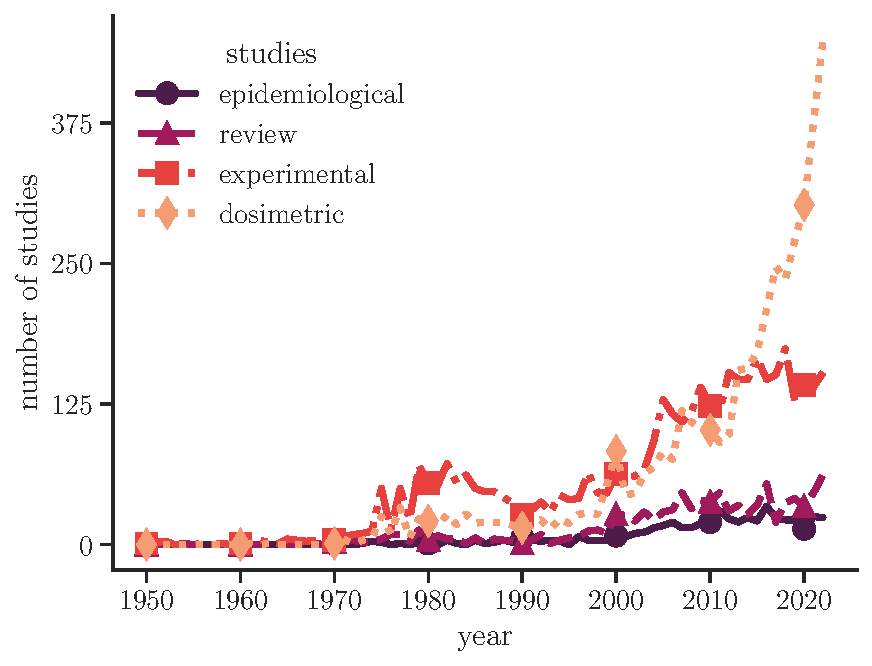
\includegraphics[width=0.8\textwidth]{artwork/research_compilation.pdf}
    \caption{Papers published between 1950 and 2022 related to research on bioeffects of radio-frequency electromagnetic fields and/or mobile communications.
    Compiled from \href{http://www.emf-portal.org}{\url{emf-portal.org}}.}
    \label{fig:research_compilation}
\end{figure}

\subsection{Scientific Basis for Limiting Exposure}
Below \SI{10}{\MHz}, induced electric fields may stimulate nerves and potentially cause dielectric breakdown of biological membranes~\cite{Swicord2008Has}.
Such and similar effects are defined as non-thermal and can be classified into four groups: resonance mechanisms, coupling with nonlinear systems, effects due to the direct action of electric and magnetic fields, and cooperative mechanisms due to interactions among several membrane components~\cite{DInzeo2009Deliverable}.
Above \SI{100}{\kHz}, the result of the interaction between induced electric fields and polar molecules or free charges within the exposed body is the kinetic energy which causes polar molecules to rotate and oscillate around their center and charges to form the electric current.
The increased kinetic energy leads to more frequent interactions and the conversion of kinetic energy into thermal energy~\cite{Foster2018Modeling}.

To evaluate heating effects, quantifying the absorbed power in exposed tissue is crucial.
It is generally considered that below \SI{6}{\GHz}, \gls{emf}s penetrate deep, whereas above this frequency, power is primarily dissipated on the surface of the tissue~\cite{Ziskin2018Tissue}.
\Cref{fig:penetration_depth} illustrates the power transmission coefficient and power penetration depth into a uniform half-plane of tissue with frequency-dependent dielectric properties of dry skin.
\begin{figure}[t]
    \centering
    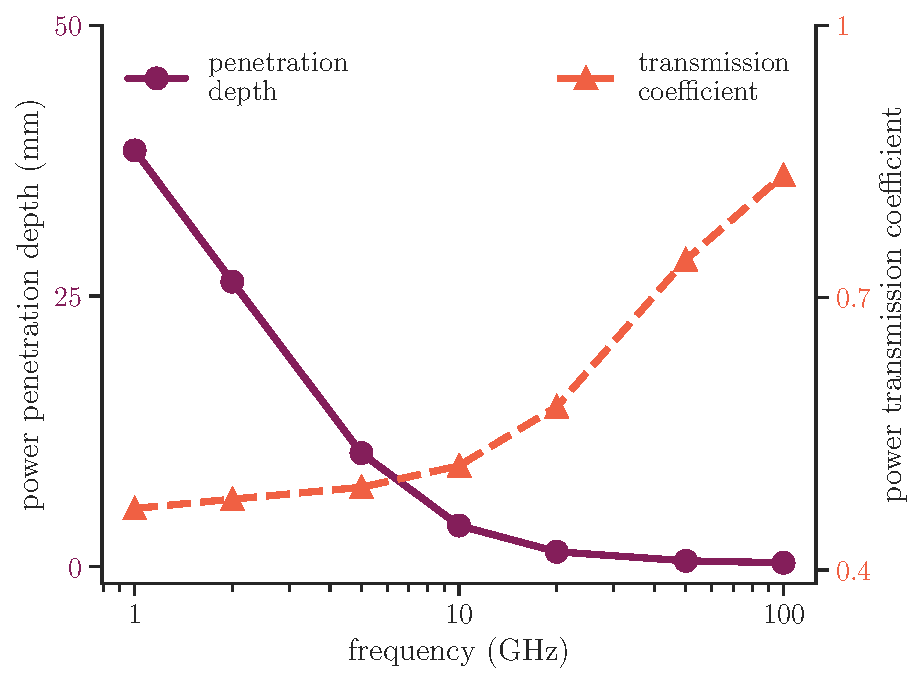
\includegraphics[width=0.8\textwidth]{artwork/penetration_depth.pdf}
    \caption{Power transmission coefficient and power penetration depth into dry skin as a function of frequency.}
    \label{fig:penetration_depth}
\end{figure}
Dielectric properties of dry skin are obtained from~\cite{Gabriel1996Compilation}.
The power penetration depth into the tissue is defined
as the distance beneath the surface at which the power density has fallen to a factor of $\nicefrac{1}{e}$ compared to the surface level, which is a half of the commonly reported wave penetration depth~\cite{Foster2016Thermal}.

Exposure limits set (operational) threshold levels to restrict temperature rise rather than focusing on absolute temperature.
Absolute temperature depends on various factors such as sex, age, thermoregulation, surrounding temperature, clothing, and work rate, which are not addressed by neither the \gls{icnirp} guidelines nor \gls{ieee} standard.
Temperature rise can be classified into steady-state and brief temperature rise.
Steady-state temperature rise gives sufficient time for heat to disperse throughout a larger tissue mass and for thermoregulatory processes to activate.
The steady-state increase of core body temperature is typically restricted to \SI{1}{\celsius}, although there is no scientific evidence for adversity even at higher temperature rise.
Due to the limited literature available, steady-state temperature rise of \SI{1}{\celsius} has been adopted in a conservative manner as it triggers significant physiological changes~\cite{Heuvel2017independent}, which are not represented as adverse health effects.

Furthermore, guidelines also specify limits for steady-state local temperature rise in specific body regions, such as the head, torso, and limbs.
For regions with normothermal temperature of \SIrange{33}{36}{\celsius}, the local temperature rise should be limited to \SI{5}{\celsius}.
In regions with higher normothermal temperature of \SIrange{36}{38.5}{\celsius}, such as the head, eyes, abdomen, thorax, and pelvis, the local temperature rise should be limited to \SI{2}{\celsius}.
These limits are based on experimental human studies~\cite{Walters2000Heating}, considering that tissue damage may occur at temperatures between \SIrange{41}{43}{\celsius}~\cite{Dewhirst2003Basic}, with the severity and likelihood of damage increasing with longer exposure times.

Lastly, rapid temperature rise can lead to inhomogeneous temperature distribution over the exposed tissue before thermoregulatory responses take effect, allowing heat dissipation within the tissue~\cite{Foster2016Thermal,Foster2017Thermal,Laakso2017Human,Kodera2018Brief}.
This topic will be discussed in more detail in the following sections.

\subsection{Basic Restrictions}
\Gls{br}s/\gls{drl}s (hereafter, only the acronym ``\gls{br}'' will be used for the sake of brevity and improved readability) have been derived from the levels of \gls{rf} \gls{emf}s that correspond to the (operational) adverse health effects.
Typically, \gls{br}s concerning \gls{rf} \gls{emf}s are frequency-dependent dosimetric quantities that are treated separately depending on the spatio-temporal scale of exposure.

For steady-state body core temperature rise, the whole-body averaged \gls{sar} is defined as the \gls{br} within the frequency range of \SI{100}{\kHz} to \SI{300}{\GHz}.
\Gls{sar} represents the rate at which energy is absorbed per unit mass by a human body when exposed to \gls{rf} \gls{emf}s.
Specifically, it quantifies the power absorbed per unit mass of tissue and is expressed in watts per kilogram.
The establishment of the whole-body averaged \gls{sar} was based on theoretical modeling and the extrapolation of findings from experimental studies conducted on various species.
Both the \gls{icnirp} and \gls{ieee} have determined a whole-body averaged \gls{sar} value of \SI{4}{\watt\per\kg}, averaged over the entire body mass and a duration of \SI{30}{\minute}, as a threshold for exposure associated with operational adverse health effects, particularly an increase in body core temperature of \SI{1}{\celsius}.
In order to account for scientific uncertainties and intervariability in the thermal physiology of occupationally exposed workers, an additional reduction or safety factor of \num{10} is applied.
Moreover, a reduction factor of \num{50} is implemented for the general public.

\Gls{sar} averaged over \SI{10}{\g} is a suitable measure for estimating the local steady-state temperature increase in tissue exposed to \gls{rf} \gls{emf}s between \SI{100}{\kHz} and \SI{6}{\GHz}.
The choice of a 10-g mass is somewhat arbitrary, as thermal energy diffuses rapidly and distributes across a larger volume, even though the initial temperature distribution may be inhomogeneous~\cite{Hirata2009correlation}.
For head and torso, a \gls{sar} value of \SI{20}{\watt\per\kg} averaged over \SI{10}{\g} and a duration of \SI{6}{\minute} align well with the threshold for (operational) adverse health effects.
A safety factor of \num{2} is applied to occupational exposure, whereas a safety factor of \num{10} is applied to the general public.
Conversely, the limbs consist of tissues with lower normothermal temperatures.
Therefore, a \gls{sar} value of \SI{40}{\watt\per\kg} averaged over \SI{10}{\g} and a duration of \SI{6}{\minute} is set instead.
Reduction factors match those for the head and torso.

At higher frequencies, the majority (up to \SI{90}{\percent}) of the total power is dissipated near the surface of the exposed tissue, for example: \SI{8}{\mm} at \SI{6}{\GHz} and \SI{0.81}{\mm} at \SI{30}{\GHz}~\cite{Sasaki2017Monte}.
Consequently, it is more appropriate to spatially average the absorbed power on the surface rather within the volume.
For local exposure at \SI{6}{\GHz}, the \gls{br} is expressed by means of the spatially averaged \gls{apd} as the most of the power is absorbed in the upper portion of a 10-g \gls{sar} cubic volume.
For dry skin of the average density of \SI{1109}{\kg\per\m\cubed}, the cubic volume corresponds to \SI{2.15}{\cm\cubed}.
Recent thermal modeling~\cite{Hashimoto2017averaging} and analytical studies~\cite{Foster2017Thermal} suggest that at the \SIrange{6}{30}{\GHz} range, exposure over a square area of \SI{4}{\cm\squared} (approximately matching the front surface area of a 10-g cube) provides a reliable correlation with maximum local temperature rise.
This finding is supported by simulations of realistic exposure scenarios~\cite{He2018RF}.
To account for narrow beam formation at higher frequencies, \gls{apd} should be averaged on the most exposed area of \SI{1}{\cm\squared} at the \SIrange{30}{300}{\GHz} range.
This ensures that the operational adverse health effect thresholds are not exceeded over smaller regions, as long as the value remains within two times that of the averaging area of \SI{4}{\cm\squared}~\cite{Foster2016Thermal}.
For both the head/torso and limb region, the operational adverse health effect threshold is reached for the spatially averaged \gls{apd} of \SI{200}{\W\per\m\squared} over a 6-min interval and a surface area of \SI{4}{\cm\squared} on the exposed region of the body.
Similar to \gls{sar}, safety factors of \num{2} or \num{10} are applied subsequently as a precautionary measure for occupational exposure or the general public, respectively.

\Gls{br}s for rapid temperature rise after a brief exposure are defined by means of the specific energy absorption at the \SI{400}{\MHz} to \SI{6}{\GHz} range as a function of time.
Much like \gls{sar}, specific energy absorption is spatially averaged over a 10-g cubic mass.
Concrete formulations and values are available elsewhere, e.g. in~\cite{ICNIRP2020Guidelines,IEEE2019Standard}.
An additional safety factor of either \num{2} and \num{10} is applied to specific energy absorption for occupational exposure or the general public, respectively.

Above \SI{6}{\GHz}, following the same reasoning as for the case of setting \gls{br}s for local steady-state temperature rise, the absorbed energy density is averaged over a square \SI{4}{\cm\squared} area of the most exposed body region of interest.
To account for focal beam exposure at the \SIrange{30}{300}{\GHz} range, averaging should be performed additionally over a square area of \SI{1}{\cm\squared} whereas the absorbed energy density should be at most twice the value for the corresponding averaging area of \SI{4}{\cm\squared}.
Again, safety factors of \num{2} and \num{10} are respectively applied for occupational exposure and the general public, respectively.

\subsection{Exposure Reference Levels}
\Gls{rl}s/\gls{erl}s (hereafter, only the acronym ``\gls{rl}'' will be used for the sake of brevity and improved readability) have been derived from a combination of computational and measurement studies to provide more practical means of demonstrating compliance by using physical quantities that are easy to assess without the need of having a human body in the measurement loop.
The measurement takes place in free space, where instead of absorbed, incident values are considered.
Within the existing literature, the term ``exposure assessment'' pertains to the evaluation of \gls{rf}-\gls{em} energy that reaches the body, while ``dosimetry'' refers to determining the absorption of \gls{rf}-\gls{em} energy within the body~\cite{Chou1996Radio}.

The \gls{rl} quantities include incident electric field strength, incident magnetic field strength, \gls{ipd}, plane-wave equivalent \gls{ipd}, incident energy density, plane-wave equivalent incident energy density, and electric current within the body, all measured outside the body.
These physical quantities serve as predictors for assessing compliance with \gls{br}s.
The accuracy of predictions is strongly related to whether external \gls{emf}s can be considered to be within the far field, radiative near field or reactive near field.
The \gls{icnirp} guidelines~\cite{ICNIRP2020Guidelines} and \gls{ieee} standard~\cite{IEEE2019Standard} have slightly different and more conservative rules for exposure in the near field compared to far field~\cite{Hirata2020Difference}.
This thesis focuses on \gls{rf}-\gls{emf} exposure within the \SIrange{6}{300}{\GHz} range, while details for determining \gls{rl}s outside this range can be found in other sources such as ``Reference levels'' chapter in the \gls{icnirp} 2020 guidelines~\cite{ICNIRP2020Guidelines} and chapter 4.3 in the \gls{ieee} C95.1-2019 standard~\cite{IEEE2019Standard}.
Within the \SIrange{6}{300}{\GHz} range, \gls{ipd} is defined as the \gls{rl} averaged over a 6-min period for local exposure, either as a peak value (at \SI{6}{\GHz}) or spatially averaged over a square area of \SI{4}{\cm\squared} above \SI{6}{\GHz}.
Additionally, above \SI{30}{\GHz}, \gls{ipd} should be averaged over a square of \SI{1}{\cm\squared} projected onto the body surface, with the restriction that it cannot exceed twice the value on the corresponding area of \SI{4}{\cm\squared}.

Compliance within the far field at \SI{6}{\GHz} requires that the peak-spatial \gls{ipd} remains below the specified value.
When appropriate, the plane-wave equivalent \gls{ipd} can be used as a substitute for the peak-spatial \gls{ipd}.
In the radiative near-field, wherein the predominant components of the \gls{emf} are those that represent a propagation of energy, compliance is solely assessed using the peak-spatial \gls{ipd}.
Conversely, in the reactive near field, \gls{rl}s are inadequate for demonstrating compliance altogether, and \gls{br}s must be utilized instead.
This is because the predominant components of the electric and magnetic field components are $\nicefrac{\pi}{2}$ out of phase and represent an exchange of reactive energy between the radiating source and surrounding medium.
Same principles apply above \SI{6}{\GHz} and up to \SI{300}{\GHz}, where compliance with prescribed limits is determined using the spatially averaged \gls{ipd} rather than the peak-spatial value.
For a comprehensive overview of \gls{rl}s for local exposure averaged over a 6-min interval within the \SIrange{6}{300}{\GHz} range, refer to~\cref{tab:rls}.
\begin{table}[b]
\begin{center}
\caption{(Exposure) reference levels averaged over a 6-min interval at the \SIrange[range-units=single,range-phrase=--]{6}{300}{\GHz} range.}
\label{tab:rls}
%\resizebox{\textwidth}{!}{%
\begin{tabular}{|c|c|c|cc|}
\hline &  &  & \multicolumn{2}{c|}{\textbf{value}${}^{*}$ \textbf{(\SI{}{\watt\per\m\squared})}} \\
\cline{4-5} \multirow{-2}{*}{\begin{tabular}[c]{@{}c@{}}\textbf{exposure}\\ \textbf{scenario}\end{tabular}} & \multirow{-2}{*}{\textbf{frequency (\SI{}{\GHz})}} & \multirow{-2}{*}{\begin{tabular}[c]{@{}c@{}}\textbf{(exposure)} \\
\textbf{reference levels}\end{tabular}} & \multicolumn{1}{c|}{ICNIRP~\cite{ICNIRP2020Guidelines}} & IEEE~\cite{IEEE2019Standard} \\
\hline & 6 &  & \multicolumn{1}{c|}{200} & 200 \\
\cline{2-2} \cline{4-5} & 6--300 &  & \multicolumn{1}{c|}{$275 \; f_G^{-0.177}$} & $274.8 \; f_G^{-0.177}$ \\ \cline{2-2} \cline{4-5} 
\multirow{-3}{*}{\begin{tabular}[c]{@{}c@{}}occupational\\ (restricted\\ environments)\end{tabular}} & 300 &  & \multicolumn{1}{c|}{100} & 100 \\ \cline{1-2} \cline{4-5} 
 & 6 &  & \multicolumn{1}{c|}{40} & 40 \\ \cline{2-2} \cline{4-5} 
 & 6--300 &  & \multicolumn{1}{c|}{$55 \; f_G^{-0.177}$} & $55 \; f_G^{-0.177}$ \\ \cline{2-2} \cline{4-5} 
\multirow{-3}{*}{\begin{tabular}[c]{@{}c@{}}general public\\ (unrestricted\\ environment)\end{tabular}} & 300 & \multirow{-6}{*}{\gls{ipd}} & \multicolumn{1}{c|}{20} & 20 \\ \hline
\end{tabular}%
%}
\end{center}
${}^{*}f_G$ stands for the frequency in \SI{}{\GHz}.
\end{table}

In \cref{fig:reference_levels}, \gls{ipd} as a function of frequency is shown within the \SIrange{6}{300}{\GHz} range.
\begin{figure}[t]
    \centering
    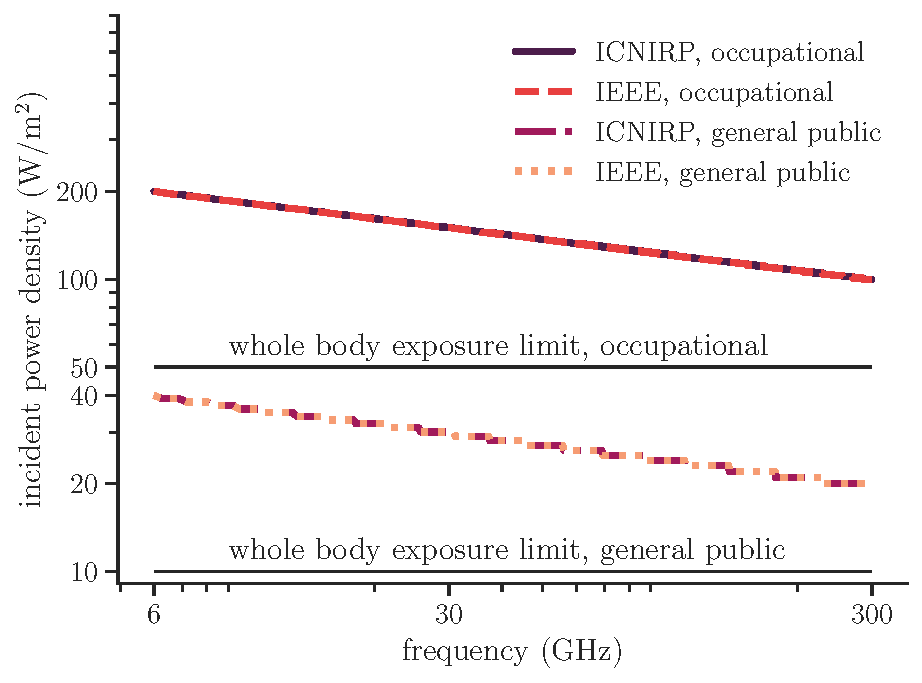
\includegraphics[width=0.8\textwidth]{artwork/reference_levels.pdf}
    \caption{Incident power density as a function of frequency for general public and occupational exposures at \SIrange{6}{300}{\GHz}.}
    \label{fig:reference_levels}
\end{figure}
Constant values of \SIlist{50;10}{\watt\per\m\squared} are prescribed for whole-body exposure in occupational and general public settings, respectively.
For local exposure at \SI{6}{\GHz} within the far field, compliance is achieved if the peak-spatial \gls{ipd} remains below the specified value.
The plane-wave equivalent \gls{ipd} can be used as a substitute when appropriate.
In the radiative near field, compliance is demonstrated by ensuring that the \gls{ipd} does not exceed the limits.
However, within the reactive near field, compliance cannot be determined based on \gls{ipd} alone; dosimetric values must be assessed instead.

The assessment of cumulative effects from simultaneous exposure to multiple frequency \gls{rf} \gls{emf}s, considering both thermal and electrical stimulation, is out of the scope of this thesis; for details on this subject, refer to~\cite{ICNIRP2020Guidelines, IEEE2019Standard}.
However, it is worth noting that in a recent computational study~\cite{Miura2021Power}, simultaneous exposure at \SIlist{2;28}{\GHz} have been evaluated using realistic antenna models.
It has been shown that the superposition effect is negligible in most cases, except in a very specific situation in which the patch antenna array and inverted-F antenna are separated by less than \SI{50}{\mm} at the antenna-body distance of \SI{5}{\mm}.

    \cleardoublepage

\chapter{GOVERNING EQUATIONS AT GIGAHERTZ RANGE}
\label{chap:3}

\section{Specific Absorption Rate}
In general, there exists a strong correlation between heating effects and the amount of the \gls{em} power that is absorbed by human tissue.
The comprehensive measure of power absorption per unit mass is commonly expressed in terms of \gls{sar}, measured in watts per kilogram.
A seminal work by Chou~\cite{Chou1975Effects}, as referenced in~\cite{Foster2022Three}, highlights the initial appearance of the term ``\gls{sar}'' within the context of his doctoral dissertation in 1975.

\Gls{sar} serves as a quantitative measure of the rate at which \gls{em} energy is either absorbed by or dissipated in a unit mass contained within a volume element,
\begin{align}
    \label{eqn:sar_1}
    \text{SAR} = \frac{\partial}{\partial t} \left( \frac{\partial W}{\partial m} \right).
\end{align}
In cases where the exposed tissue is of constant density, $\rho$, the aforementioned relationship can be represented as
\begin{align}
    \label{eqn:sar_2}
    \text{SAR} = \frac{\partial}{\partial t} \left( \frac{\partial W}{\rho \; \partial V} \right),
\end{align}
where $V$ stands for the observed volume element.

Biological tissue is regarded as a magnetically transparent and lossy medium, characterized by a frequency-dependent relative complex dielectric permittivity, $\varepsilon^*$, and relative permeability, $\mu_r = 1$~\cite{Sasaki2014Measurement}.
Consequently, under practical circumstances, \gls{sar} can be assessed by using the following expression:
\begin{align}
    \label{eqn:sar_3}
    \text{SAR} = \frac{\sigma \; \left| \mathbf{E} \right|^2}{2 \rho}.
\end{align}
Here, $\sigma$ represents the conductivity of the tissue measured in siemens per meter, while $\mathbf{E}$ is the peak value of the electric field at a specific point within tissue.

In cases of brief exposure with negligible heat loss, the temperature rise can be approximated as
\begin{align}
    \label{eqn:sar_4}
    \text{SAR} = C \; \frac{\partial T}{\partial t},
\end{align}
where $C$ represents specific heat capacity $\left[ \SI{}{\joule\per\kg\per\celsius} \right]$, and $T$ denotes the temperature measured in degrees Celsius.
However, in realistic exposure scenarios that cannot be approximated by using homogeneous models, heat loss becomes significant due to the rapid diffusion caused by active thermoregulatory mechanisms.
Consequently, when \gls{sar} is used as a surrogate for temperature rise, it is necessary to spatially average it either over the whole body or, in the case of local exposure, over the volume of tissue weighing \SI{10}{\g}~\cite{McIntosh2011SAR}.

The volume-averaged \gls{sar} over \SI{10}{\g},
\begin{align}
    \text{10-g SAR} = \frac{1}{2} \; \int_{V_\text{10 g}} \frac{\sigma \; \left |\mathbf{E} \right|^2}{\rho} \; \mathrm{d}V,
\end{align}
has been shown to correlate with temperature rise well up to \SI{6}{\GHz}, regardless of whether a homogeneous cubical or a morphologically accurate body model is employed~\cite{Hirata2009correlation}.
In scenarios where simplistic tissue models are utilized, the peak-spatial \gls{sar} can also serve as an indicator of temperature rise, particularly in the frequency bands of \SIlist{150;400;900}{\MHz}.
This observation is supported by investigations employing a realistic \gls{3-d} human body model~\cite{Hirata2006Correlation}.
At higher frequencies, particularly above \SI{6}{\GHz}, the correlation between peak-spatial \gls{sar} and maximum temperature rise is only modest for realistic exposure scenarios involving morphologically accurate body models~\cite{Morimoto2016Relationship}.

In the context of whole-body exposure, assessment of the whole-body averaged \gls{sar} is contingent upon factors such as the spatial distribution of the internal electric field, electric conductivity of tissue, and tissue density.
Thus, the whole-body averaged \gls{sar} can be defined as the ratio of the total power absorbed in the whole body and the whole body mass:
\begin{align}
    \label{eqn:sar_wb}
    \text{whole-body SAR} = \frac{1}{2} \; \int_{V_\text{wb}}\frac{\sigma \; \left |\mathbf{E} \right|^2}{\rho} \; \mathrm{d}V,
\end{align}

Several numerical analyses have been conducted to investigate various averaging schemes in terms of their efficacy in predicting local temperature rise~\cite{Hirata2009correlation,McIntosh2011SAR}.
Consensus has been reached regarding the suitability of a cubic averaging mass of \SI{10}{\g} as an appropriate equivalent volume for spatial averaging up to \SI{6}{\GHz}, regardless of the tissue type.
It is worth emphasizing that a 10-g volume corresponds approximately to \SI{2.15}{\cm\cubed} cube, assuming that the density of exposed tissue is the same as that of water, i.e., \SI{1000}{\kg\per\m\cubed}.

On average, the time required to reach a steady state for the case of the whole body exposure is \SI{30}{\minute} minimum.
Conversely, for localized exposure, duration of \SI{6}{\minute} is deemed sufficient.
The consideration of temporal averaging for whole-body exposure is based on both analytical approximations provided in the \gls{icnirp} guidelines~\cite{ICNIRP2020Guidelines} and empirical studies~\cite{Hirata2008FDTD,Nelson2013High}.
The time constant is governed by the rate of heat exchange between the core of the body and the surrounding environment~\cite{Adair2003Thermoregulatory}.
The temporal averaging for localized exposure is more intricate as it depends on two distinct factors, such as the rate of convective heat exchange by blood flow and conduction of heat from the exposed area~\cite{Foster2017Thermal}.
Simple analytical models~\cite{Foster2017Thermal} and a detailed numerical analysis~\cite{Morimoto2017Time} indicate that the overall dissipation of heat from an exposed region is primarily governed by thermal convection through blood flow.
In turn, thermal convection depends on multiple factors, but is generally accepted that after \SI{6}{\minute}, a steady state is reached in most exposure scenarios.

\section{Transition to Area-Averaged Dosimetric Quantities}
In 1998 version of the \gls{icnirp} guidelines~\cite{ICNIRP1998Guidlines}, \gls{sar} was used up to \SI{10}{\GHz}, whereas the power density was used above this transition frequency.
However, in 2005 version of the \gls{ieee} standard~\cite{IEEE2005Standard}, the transition frequency was adjusted to \SI{3}{\GHz}.
This discrepancy resulted in a discontinuity in the exposure limits at the transition frequency~\cite{Colombi2015Implications}.
Recent studies demonstrated that \gls{sar} no longer serves as an appropriate surrogate for predicting local temperature rise above \SI{6}{\GHz}, particularly at \gls{mmw}.
This is primarily due to the fact that at such high frequencies, \gls{em} energy is deposited predominantly in cutaneous tissue~\cite{Ziskin2018Tissue,Zhadobov2011Millimeter}.
With an increase in frequency, the \gls{emf} penetration depth decreases, resulting in a more superficial distribution of \gls{em} energy.
Therefore, the power density absorbed in the skin provides a better estimation of the maximum temperature rise on the surface of the exposed body at the \SIrange{6}{300}{\GHz} range~\cite{Funahashi2018Area-averaged}.

The need for the harmonization between the volume-averaged \gls{sar} and area-averaged power density and determination of a break-point between exposure limits was recognized as early as 2011~\cite{McIntosh2011SAR}.
In this study, authors argue that the combined results of simple planar and complex body modeling did not offer a clear indication of which metric exhibited a stronger correlation with the induced temperature rise from \gls{rf} heating at the \SIrange{3}{10}{\GHz} range.
However, from a practical standpoint, \SI{6}{\GHz} was identified as the transition frequency due to the ease of assessing spatially averaged power density by comparison to volume-averaged \gls{sar}.

Based more recent analytical~\cite{Foster2016Thermal,Foster2017Thermal,Ziskin2018Tissue} and numerical studies~\cite{Hirata2019Setting}, the transition frequency has been set to \SI{6}{\GHz} in the recent updates of the \gls{icnirp} guidelines and \gls{ieee} standard, leading to the long-awaited harmonization.

\subsection{Absorbed/Epithelial Power Density}
Dissipation of power density within the tissue exhibits an exponential decline from the surface towards deeper regions.
Thus, the spatially averaged \gls{apd} on the surface is defined as
\begin{align}
    \label{eqn:apd}
    S_\text{ab} = S(z=0) \; \int_{z=0}^{z_\text{max}} e^{ -\nicefrac{2z}{\delta}} \; \mathrm{d}z,
\end{align}
where $S(z=0)$ represents the specific \gls{apd} averaged on the exposed surface, $\delta$ stands for the perpendicular penetration depth into the tissue (along the $z$-axis in this context), whereas $z_\text{max}$ denotes the depth of the exposed tissue which must be sufficiently large to compensate for $\delta$.

The specific \gls{apd} at $z=0$, averaged over area $A$ is expressed as
\begin{align}
    \label{eqn:specific_apd}
    S(z=0) = \frac{1}{A} \; \iint_A \rho(x, y, 0) \; \text{SAR}(x, y, 0) \; \mathrm{d}x \mathrm{d}y.
\end{align}

To illustrate the exponential decay, let's consider the following example.
Firstly, \num{1000} values are sampled from a continuous uniform distribution constrained within the range from \SI{0}{\watt\per\m\squared} and the maximum permissible \gls{ipd} at \SIlist{10;30;60;100}{\GHz}.
The mean and standard deviation of these sampled values are calculated.
Next, we estimate the specific area-averaged \gls{apd} using the following expression:
\begin{align}
    \label{eqn:specific_apd_approx}
    S(z=0) = T \cdot \text{IPD}.
\end{align}
Here, $T$ denotes the transmission coefficient, which is defined as
\begin{align}
    \label{eqn:transmittance}
    T = 1 - \left| \Gamma \right|^2.
\end{align}
The reflection coefficient,  $\Gamma$, is derived from the dielectric properties of the tissue, shape of the body surface, incident angle and polarization.
For this purpose, we consider a scenario involving a plane wave with normal incidence onto a planar, dry skin half-space.
The dielectric properties are characterized by the relative complex permittivity~\cite{Wu2015human},
\begin{align}
    \label{eqn:rel_complex_permittivity}
    \varepsilon^* = \varepsilon' + j \; \varepsilon'',
\end{align}
where
\begin{align}
    \varepsilon'' = \frac{\sigma}{2 \pi f \varepsilon_0}.
\end{align}
The value of $\varepsilon'$ is extracted from~\cite{Gabriel1996Compilation} at the corresponding frequency. 
This sampling procedure is repeated \num{1000} times to acquire the expected specific \gls{apd} within the range of values that can are approximated from the range of \gls{ipd}s.
Finally, in~\cref{fig:power_density_absorption}, the intensity of the power density at $z=\SI{0}{\mm}$ is depicted with a solid line, whereas the value of the power density absorbed at a depth of \SI{1}{\mm} into the dry skin is represented by a dashed line.
\begin{figure}[ht]
    \centering
    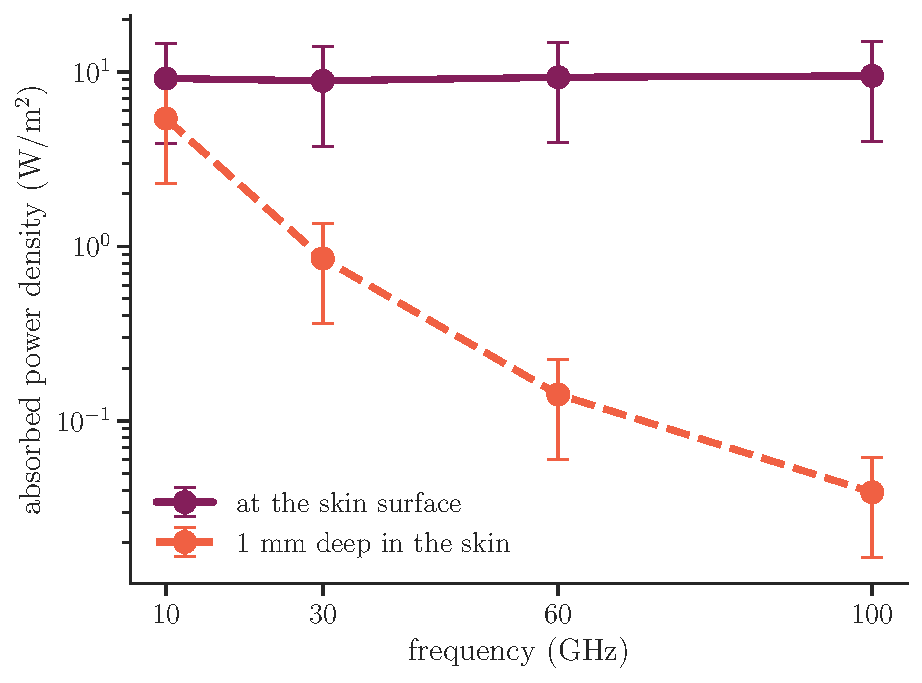
\includegraphics[width=0.8\textwidth]{artwork/power_density_absorption.pdf}
    \caption{Power density as a function of frequency at the skin surface (solid line) and at \SI{1}{\mm} depth in homogeneous dry skin (dashed line).}
    \label{fig:power_density_absorption}
\end{figure}
With an increase in frequency, and for \gls{ipd} bounded between \SI{0}{\watt\per\m\squared} and the maximum allowable value~\cite{ICNIRP2020Guidelines,IEEE2019Standard}, the power density at the surface remains relatively constant at approximately \SI{9}{\watt\per\m\squared}.
However, even at a depth of \SI{1}{\mm} perpendicular into the skin, $S_\text{ab}$ drops respectively by \SIlist{40.98;90.39;98.48;99.59}{\percent} at \SIlist{10;30;60;100}{\GHz} by using the corresponding surface value as a reference.

In the updated version of the \gls{icnirp} guidelines~\cite{ICNIRP2020Guidelines} and \gls{ieee} standard~\cite{IEEE2019Standard}, two definitions of the spatially averaged \gls{apd} have been adopted, both stemming from the Poynting theorem.
The first definition of is given in terms of \gls{tpd}~\cite{Funahashi2018Area-averaged}
\begin{align}
    \label{eqn:tpd}
    \text{TPD}(x, y) = \int_{z = 0}^{z_\text{max}} \rho(x, y, z) \; \text{SAR}(x, y, z) \; \mathrm{d}z,
\end{align}
spatially averaged across the exposed surface of tissue, $A$
\begin{align}
    \label{eqn:apd_1}
    S_\text{ab, v} = \frac{1}{A} \iint_{A} \text{TPD}(x, y) \; \mathrm{d}A.
\end{align}
The tissue surface is positioned at $z = 0$, whereas $z_\text{max}$ should be sufficiently greater than the penetration depth.
The second formula is given as the spatially averaged power density flux on the exposed surface
\begin{equation}
    \label{eqn:apd_2} 
    S_\text{ab, s} = \frac{1}{2A} \iint_{A} \Re \big[\mathbf{E}(x, y) \times \mathbf{H}^*(x, y) \big] \; \mathbf{\hat n} \; \mathrm{d}A
\end{equation}
where $\mathbf{E}$ and $\mathbf{H}$ are peak values of the complex phasor electric and magnetic field on the surface, respectively, $\Re$ denotes the real part of the vector field, and the asterisk represents the complex conjugate operator.
Integral variable vector, $\mathbf{\hat n} \; \mathrm{d}A$, is set perpendicularly to the exposed surface, where  $\mathbf{\hat n}$ corresponds to the unit normal vector to the surface.

It is outlined in~\cite{Hashimoto2017averaging} that a square \SI{4}{\cm\squared} evaluation surface provides a close approximation to maximum temperature rise due to \gls{rf} heating above \SI{6}{\GHz}.
The results are based on the heating factor, the ratio between the spatially averaged \gls{apd} and maximum temperature rise, computed on a a multiple-layer tissue model exposed to three different sources of \gls{emf}s: the plane wave, a dipole antenna, and an antenna array.
The schematic of the exposed tissue is shown in~\cref{fig:averaging_surface}.
\begin{figure}[t]
    \centering
    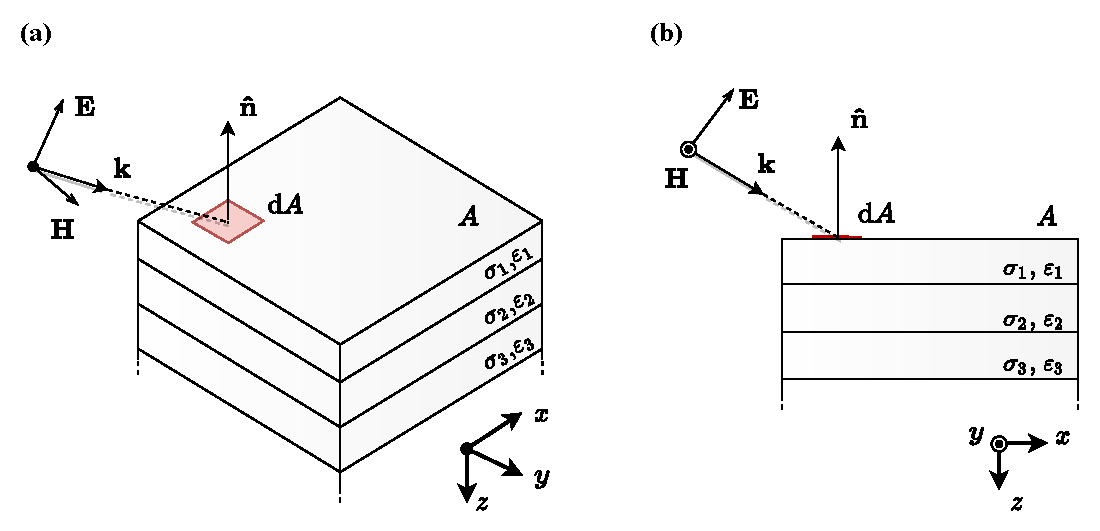
\includegraphics[width=\textwidth]{artwork/averaging_surface.pdf}
    \caption{Evaluation surface on a multiple-layer tissue-equivalent block model: (a) isometric projection, (b) orthographic projection.}
    \label{fig:averaging_surface}
\end{figure}
The area of \SI{4}{\cm\squared} achieves consistency with the volume-averaged dosimetric quantities below \SI{6}{\GHz} as the front facing surface of 10-g cubic volume is approximately of the same area ($2.15 \times 2.15$ \SI{}{\cm\squared} assuming constant tissue density of \SI{1000}{\kg\per\m\cubed}).
\begin{figure}[t]
    \centering
    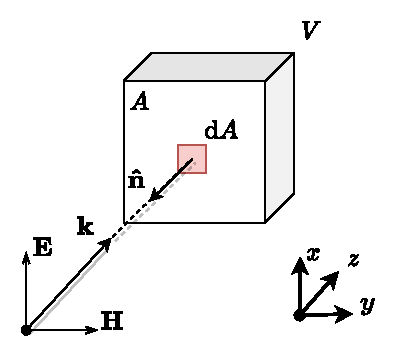
\includegraphics[width=0.42\textwidth]{artwork/averaging_volume.pdf}
    \caption{A 10-g cubic volume for assessment of local exposure to radio-frequency electromagnetic fields below \SI{6}{\GHz}.}
    \label{fig:averaging_volume}
\end{figure}

At frequencies above \SI{30}{\GHz}, the area of \SI{4}{\cm\squared} is not suitable for spatial averaging because of the possibility of inhomogeneous field distribution.
Therefore, \gls{apd} should be averaged on square \SI{1}{\cm\squared} evaluation plane to capture the focused beams.

\subsection{Equivalence of Absorbed/Epithelial Power Density Definitions}
In~\cref{eqn:apd_2}, the cross product between peak values of the complex phasor electric and magnetic field represents the power density vector field whose direction is perpendicular to the incident surface.
Essentially, this cross product represents the Poynting vector, given in~\cref{eqn:poynting-vector}.

The surface integral of the normal component of the time-averaged Poynting vector on the exposed surface results in a scalar value, which corresponds to the overall flux passing through that surface.
The divergence theorem, commonly referred to as the Gauss-Ostrogradsky theorem, establishes a relationship between the flux of a vector field through a closed surface and the divergence of a field within an enclosed volume.
In other words, it states that the surface integral of a vector field across a closed surface is equivalent to the volume integral of the divergence within the region enclosed by that surface.

Given the aforementioned principles, it can be deduced from the Poynting theorem, given in~\cref{eqn:poynting-theorem}, that the definitions of the spatially averaged \gls{apd} are equivalent if the surface surrounding a particular volume of tissue is closed and that there are no active sources within this volume.

In both definitions, it is assumed that the Poynting vector is averaged in time and is given in its corresponding phasor notation.
However, the Poynting vector in the time-harmonic variation is written as
\begin{align}
    \label{eqn:poynting-vec-time-harmonic}
    \mathcal{P} &= \mathcal{E} \times \mathcal{H} \notag\\
                &= \Re \left( \mathbf{E} \; e^{j \omega t} \right) \times \Re \left( \mathbf{H} \; e^{j \omega t} \right) \notag\\
                &= \frac{1}{2} \; \left( \mathbf{E} \; e^{j \omega t} + \mathbf{E}^*  \; e^{-j \omega t} \right) \times \frac{1}{2} \; \left( \mathbf{H} \; e^{j \omega t} + \mathbf{H}^*  \; e^{-j \omega t} \right) \notag\\
                &= \frac{1}{2} \; \Re \left( \mathbf{E} \times \mathbf{H}^* \right) + \frac{1}{2} \; \Re \left( \mathbf{E} \times \mathbf{H} \; e^{2j \omega t} \right), 
\end{align}
where $t$ is the time domain, and the normalization factor $\nicefrac{1}{2}$ appears as \gls{emf} components are given by their corresponding peak values.
From \cref{eqn:poynting-vec-time-harmonic}, the time-averaged Poynting vector is then written as
\begin{align}
    \label{eqn:poynting-vec-time-avg}
    \mathbf{P} = \frac{1}{2} \; \Re \left( \mathbf{E} \times \mathbf{H}^* \right).
\end{align}

The time-averaged total power crossing a \gls{2-d} surface in \gls{3-d} space can then be written as
\begin{align}
    \label{eqn:poynting-flow}
    P_\text{tot} &= \oint_S \mathbf{P} \; \mathrm{d}\mathbf{S} \notag\\
                 &= \frac{1}{2} \; \oint_S \Re \big( \mathbf{E} \times \mathbf{H}^* \big) \; \mathbf{\hat n} \; \mathrm{d}S.
\end{align}
Once the total power is spatially averaged on the exposed surface, $\nicefrac{P_\text{tot}}{A}$, the resulting quantity is equivalent to a radiated power density uniformly distributed over the averaging area $A$ and crossing this surface.

Now, by enforcing the divergence theorem onto the Poynting flow given in \cref{eqn:poynting-flow} through any closed surface, $S$, bounding an arbitrary volume, $V$, under the assumption that there are no active sources inside that volume, the above expression can be rewritten as
\begin{align}
    P_\text{tot} &= \frac{1}{2} \; \iiint_V \nabla \left [ \Re \left( \mathbf{E} \times \mathbf{H}^* \right) \right] \; \mathrm{d}V \notag\\
                 &= -\frac{1}{2} \; \iiint_V \sigma \; |\mathbf{E}|^2 \; \mathrm{d}V.
\end{align}
By separating the total power loss in the expression above into the surface integration of the line integral and, subsequently, averaging it spatially across the surface facing the direction of the impinging \gls{em} wave as
\begin{align}
    \frac{P_\text{tot}}{A}  &= \frac{1}{2A} \iiint_V \sigma \; |\mathbf{E}|^2 \; \mathrm{d}V \notag\\
                            &= \frac{1}{2} \; \iint_A \int_z \sigma \; |\mathbf{E}|^2 \; \mathrm{dA} \mathrm{d}z,
\end{align}
the above expression matches the definition of the spatially averaged \gls{apd} given in~\cref{eqn:apd_1}.

Finally, it is clear that the definitions are equivalent if the averaging surface for $S_\text{ab, s}$ is closed and free of sources.
This condition must be met to account for the power deposited within the volume of interest.
This means that $S_\text{ab, s}$, given as the surface integral of the vector field in~\cref{eqn:apd_2}, should take into account the entire closed surface surrounding the exposed volume and not only on the directly exposed, i.e., the front surface facing only the direction of the impinging \gls{em} wave (\cref{fig:averaging_volume}).
As this is not the case, it should be expected that $S_\text{ab, v}$ will always yield values greater than $S_\text{ab, s}$.
However, above \SI{6}{\GHz}, the power penetration depth is at most about \SI{8}{\mm}, which makes this difference only marginal.
Therefore, it may be disregarded in practice as the overall contribution of the absorption in deeper tissues is less then \SI{10}{\percent}~\cite{Li2023Calculated}.

\section{Incident Power Density}
\gls{ipd} serves as the \gls{rl} in the \gls{icnirp} guidelines~\cite{ICNIRP2020Guidelines} and the \gls{erl} in the \gls{ieee} standard~\cite{IEEE2019Standard}.
It is defined as the magnitude of the time-averaged Poynting vector, as expressed in the following equation:
\begin{align}
    \label{eqn:ipd}
    S_\text{inc} = \left| \mathbf{E} \times \mathbf{H}^* \right|.
\end{align}
For far-field exposure, \gls{ipd} can be simplified to the following expression:
\begin{align}
    \label{eqn:ipd-far-field}
    S_\text{inc} = \frac{\left| \mathbf{E} \right|^2}{Z_0} = \left| \mathbf{H} \right|^2 \; Z_0.
\end{align}
where $Z_0$ represents the characteristic impedance of free space.
Herein, the field components are treated as \gls{rms} values.

The approximation in~\cref{eqn:ipd-far-field} is a valid if the conditions of the far field are met.
This generally applies during the assessment of whole-body exposure or local exposure above \SI{6}{\GHz}, provided that the separation distance from the antenna is greater than $\nicefrac{\lambda}{2 \pi}$, where $\lambda$ denotes the wavelength of the incident field.
This distance effectively predicts the margin between the reactive and radiative near field~\cite{Carrasco2019Exposure}.
The plane-wave reflection coefficient, $\Gamma$, can be employed to establish a correlation between the incident and absorbed \gls{emf}s in the far field
\begin{align}
    \label{eqn:ipd-corr}
    S_\text{inc} = \frac{S_\text{ab}}{1 - \left| \Gamma \right|^2}.
\end{align}
However, further considerations are required for the near field.

In the far field, the Poynting vector is entirely real, and the direction of the flux remains constant over time.
On the other hand, in the near field of an antenna, this is no longer the case as reactive components of the field may contribute to the overall absorption of energy in the exposed body~\cite{Kuster1992Energy}.
Consequently, all components of the Poynting vector should be considered which makes the correlation-based formula outlined in \cref{eqn:ipd-corr} no longer accurate.

Both the \gls{icnirp} guidelines~\cite{ICNIRP2020Guidelines} and \gls{ieee} standard~\cite{IEEE2019Standard} state that the \gls{rl}s cannot be used to determine compliance in the reactive near field and \gls{br}s should be assessed instead.
Nevertheless, in the recent \gls{ieee} Guide for the definition of the \gls{ipd} to correlate surface temperature rise~\cite{IEEE2021Guide}, two distinct definitions of the \gls{ipd} have been analyzed even in the near field.

The first one is the surface-normal propagation-direction power density into the evaluation surface,
\begin{align}
    \label{eqn:ipd-normal}
    S_\text{inc, n} = \frac{1}{2 A} \; \iint_A \Re \left( \mathbf{E} \times \mathbf{H}^* \right) \; \mathbf{\hat n} \; \mathrm{d}A.
\end{align}
Here $\mathbf{E}$ and $\mathbf{H}$ represents the peak values of the complex phasor electric and magnetic field in free space, respectively.

The second definition takes into account the total propagating power density into the evaluation surface,
\begin{align}
    \label{eqn:ipd-magnitude}
    S_\text{inc, tot} = \frac{1}{2A} \iint_A \left | \Re \left( \mathbf{E} \times \mathbf{H}^* \right) \right| \; \mathrm{d}A.
\end{align}

Both definitions imply spatial averaging over the evaluation surface of area $A$.
The evaluation surface is defined as a square projection of the exposed region of tissue, where, unlike in the case of the spatially averaged \gls{apd}, incident components of the complex phasor electric and magnetic field are considered (\cref{fig:averaging_surface_fs}).
\begin{figure}[t]
    \centering
    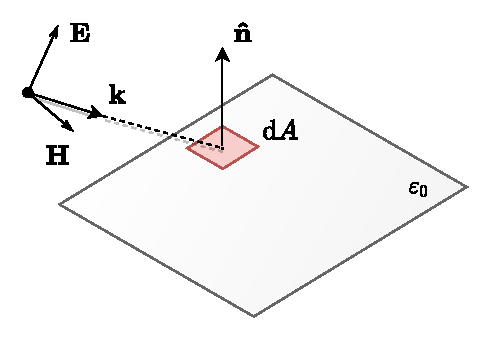
\includegraphics[width=0.46\textwidth]{artwork/averaging_surface.fs.pdf}
    \caption{Evaluation surface in free space for the averaging of the incident power density.}
    \label{fig:averaging_surface_fs}
\end{figure}

When the power density is assessed in the near field of a radiating source, the tangential components of the Poynting vector are not negligible compared to its surface-normal components.
The definition of the spatially averaged \gls{ipd} via its norm is shown to be slightly better correlated with maximum temperature rise.
However, this has been tested only considering several exposure scenarios in~\cite{IEEE2021Guide} and the overall analysis has shown that the observed difference is marginal and can mainly be attributed to near-field conditions as both definitions correlate well with temperature rise (Pearson's $r$ above 0.7).

\section{State of Research}
Choosing an appropriate spatial averaging technique is crucial for computing power density distribution on the surface on the exposed tissue.
The \gls{fdtd} method~\cite{Sullivan1987Use} is the standard numerical method of choice in numerical dosimetry for \gls{rf}-\gls{emf} simulations, owing to the advent of polished commercial software~\cite{Hirata2021Human}.
However, accurate power density values at \gls{5g} frequencies, including \gls{mmw}, on conformal surfaces of nonplanar body parts require structural rather than the grid-like spatial domain discretization~\cite{Poljak2018conformal}.
In regular grid cases, the surface is implicitly reconstructed using cubical cells, approximating spatial averaging as the sum of cell contributions.
In structural mesh cases, the surface is reconstructed using \gls{2-d} simplices and efficient quadrature schemes~\cite{Dunavant1985High,Dunavant1985Economical}.

The approach presented in this thesis does not require any priors related to positional relationship of points considering which the power density is to be spatially averaged.
Rather, it takes unorganized point set (points sampled on the nonplanar evaluation surface) as an input and estimates the unit normal in each point together with the size of the overall conformal averaging area.
From here, the spatial averaging is performed by approximating surface integrals in \gls{2-d} projected space (either by using close-form analytical formulas for the cylinder and sphere or by using the \gls{pca} for anatomical models).
More details are available in subsequent chapters.

The current state of research is reviewed based upon the available studies accessible through the EMF-portal platform.
The EMF-portal effectively summarizes scientific research data on various effects of \gls{emf}s on the human body.
The core of the EMF-portal is the literature database with \num{38786} publications and \num{7002} summaries of individual scientific studies\footnote{The total number of papers in the database was read on 2023, May 30th at: \url{https://www.emf-portal.org/en}}.

The following query was used to extract relevant studies:
\begin{verbatim}
    (power OR "power density")
    AND (average OR averaged OR area OR spatially)
    AND year=x
    AND (topic=technical_dosimetric
         OR topic=law_recommendation_guideline
         OR topic=review_survey_summary)
    AND (frequencyRange=radio_frequency
         OR frequencyRange=mobile_communications)
\end{verbatim}
where keywords are either ``power'' or ``power density'' together with either ``average'', ``averaged'', ``area'' or ``spatially''.
Keywords such as ``incident'', ``transmitted'', ``absorbed'' or even ``epithelial'' have been deliberately omitted in order to include both exposure assessment and computational dosimetry studies in the consideration regardless of authors' preference of terminology.
Additionally, the selected topics include technical dosimetry studies, laws, recommendation documents or guidelines associated with the aforementioned keywords, and review studies.
Finally, the selected frequency range includes all bands that are classified within \gls{rf} and mobile communications (above \SI{10}{\MHz}).

The purpose here is to review only the studies related to spatial averaging of power densities on the surface of the exposed tissue above \SI{6}{\GHz}.
Thus, the studies which refer to the \SIrange{6}{300}{\GHz} range are manually extracted, taking into account the publication year of each research paper from 1998 (the year of the previous version of the \gls{icnirp} guidelines~\cite{ICNIRP1998Guidlines}) to 2023 (the year of writing the thesis).
A special emphasis is on the most recent studies, written after 2019/2020, which coincide with the introduction of the spatially averaged \gls{apd} as the \gls{br} for limiting local exposure to \gls{emf}s at the \SIrange{6}{300}{\GHz} range.

In the 1998 edition of the \gls{icnirp} guidelines~\cite{ICNIRP1998Guidlines}, exposure limits \SI{10}{\GHz} were established based on the spatially averaged \gls{ipd} on a projected square-shape \SI{20}{\cm\squared} area.
Unrestricted and restricted (occupational) exposure corresponded to values of \SIlist{10;50}{\watt\per\meter\squared}, respectively.
Furthermore, local exposure was quantified by spatially averaging \gls{ipd} on the projected square-shape \SI{1}{\cm\squared} area, with limits of \SIlist{200;1000}{\watt\per\meter\squared} for unrestricted and restricted (occupational) exposure, respectively.

Contrary, the 1999 edition of the \gls{ieee} standard~\cite{IEEE1999Standard} defined maximum permissible exposure in terms of either the \gls{rms} electric and magnetic field strength, equivalent plane-wave power densities, and induced currents within the human body.
Above \SI{6}{\GHz}, restrictions for local exposure of specific body parts were determined by using the spatially averaged \gls{ipd}.
The limit for restricted exposure was set to \SI{100}{\watt\per\meter\squared}, whereas for unrestricted exposure, it varied with frequency up to \SI{15}{\GHz} and was fixed at \SI{100}{\watt\per\meter\squared} above \SI{15}{\GHz}.
These values were derived upon the steady-state volume-averaged \gls{sar}, with spatial averaging achieved by computing the \gls{rms} value of \gls{ipd} over an area equivalent to the vertical cross section of the human body at a minimum distance of \SI{20}{\cm\squared} from any object.

The 2005 edition of the \gls{ieee} standard~\cite{IEEE2005Standard} established an exposure limit in terms of the spatially averaged \gls{ipd} of \SI{10}{\watt\per\meter\squared} for unrestricted exposure at \SIrange{3}{10}{\GHz} range.
The power density should be spatially averaged over a contiguous area corresponding to $100 \cdot \lambda^2$, where $\lambda$ represents the wavelength of the incident \gls{emf}.
Moreover, within the \SIrange{3}{30}{\GHz} range, the peak-spatial \gls{ipd} was defined as $18.56 \cdot f_G^{0.699}$, whereas above above \SI{30}{\GHz}, it was set to \SI{200}{\watt\per\m\squared}.
Here, $f_G$ denotes the frequency of the \gls{emf}s in gigahertz.
The specific details regarding the averaging area and spatial sampling procedure for power density were not explicitly specified in the latter case.


\Cref{tab:summary_1998_2018} provides a concise overview of studies published between 1998 and 2017 that address the averaging of power densities, with most of these studies adopting the spatial averaging techniques outlined in~\cite{ICNIRP1998Guidlines}, with some exceptions of note.
\begin{sidewaystable}[ht]
\begin{center}
\caption{Summary of the studies published between 1998 and 2017 related to spatially averaged power densities.}
\label{tab:summary_1998_2018}
\begin{tabularx}{\textwidth}{|X|X|X|X|X|}
\hline
\textbf{Study} & \textbf{Scope} & \textbf{Exposure scenario} & \textbf{Methods} & \textbf{Averaging scheme} \\
\hline
Hirata et al. (2000)~\cite{Hirata2000Temperature} & investigation of a temperature hot-spot formation in the human eye and its dependence on \gls{sar} and additional variables & human eye voxel model exposed to plane wave (\SI{50}{\watt\per\meter\squared}) at \SIrange{0.6}{6}{\GHz} & \gls{fdtd} with the maximum cell size of $\nicefrac{\lambda}{10}$; $\lambda$ is the shortest wavelength in considered exposure scenarios & \gls{rms} of \gls{ipd} on surface approximately equivalent to the vertical cross-section (projected area) of the eye with a volume of \SI{9.9}{\cm\cubed} \\
\hline
Walters et al. (2000)~\cite{Walters2000Heating} & conduction of measurements for thermal pain thresholds; development of the \gls{1-d} thermal model & a human subject's back briefly exposed to \gls{rf} \gls{emf}s (\SI{18}{\kW\per\meter\squared}) at \SI{94}{\GHz} at the distance of \SI{188}{\cm} & readings at \SI{5}{\mm} increments over the evaluation plane which corresponds to a projection of a subject's back & mean value of the power density within the most exposed region (i.e., where \SI{90}{\percent} of the total power density is distributed) \\
\hline
Faraone et al. (2000)~\cite{Faraone2000Estimation} & estimation of the spatially averaged \gls{ipd} in the vicinity of cellular base-station antennas & free space field evaluation based on the dipole and collinear array antenna at different separation distances & analytical formulations & analytical formulations that estimate a single-point worst case measure\\
\hline
Anderson et al. (2010)~\cite{Anderson2010SAR}, McIntosh and Anderson (2010)~\cite{McIntosh2010SAR} & definition of the appropriate exposure metric at the \SIrange{1}{10}{\GHz} range and the transition frequency from \gls{sar} to \gls{ipd} & simple multiple-layer block and realistic human head voxel models exposed to a plane wave and dipole antennas at \SI{10}{\mm} separation distance & \gls{fdtd} with the maximum cell size of $\nicefrac{\lambda}{10}$; $\lambda$ is the shortest wavelength in considered exposure scenarios & peak value of \gls{ipd} for the block model; \gls{rms} of \gls{ipd} averaged on a square \SI{20}{\cm\squared} projection for head models\\
\hline
Colombi et al. (2015)~\cite{Colombi2015Implications}, Thors et al. (2016)~\cite{Thors2016Exposure}, Xu et al. (2017)~\cite{Xu2017Understanding} & harmonization of the transition frequency for \gls{br}s between existing exposure limits & various \gls{5g} antennas (dipoles and patch arrays) in free space & \gls{fem} & surface integration of either the normal component or the magnitude of the real part of the Poynting vector on a square \SI{20}{\cm\squared} evaluation surface\\
\hline
\end{tabularx}
\end{center}
\end{sidewaystable}

In~\cite{Hashimoto2017averaging}, the relationship between the averaging area for \gls{ipd} and maximum temperature rise has been investigated by employing a tissue-equivalent multiple-layer model.
Various \gls{emf} sources spanning the \SIrange{3}{300}{\GHz} range, including the plane wave, half-wavelength dipole, and dipole array, have been utilized.
This study demonstrates that more than \SI{70}{\percent} of the incident power is absorbed within a \SI{4}{\cm\squared} region.
Consequently, a square-shape averaging area of \SI{4}{\cm\squared} has been proposed as a suitable metric for correlating with maximum temperature rise, assuming a nearly uniform field distribution across the corresponding surface area.
However, for frequencies above \SI{30}{\GHz}, an additional averaging of \SI{1}{\cm\squared} has been recommended to account for localized beam formation.
These findings have been subsequently incorporated in the 2019 edition of the \gls{ieee} standard~\cite{IEEE2019Standard} and the 2020 edition of the \gls{icnirp} guidelines~\cite{ICNIRP2020Guidelines}.

Furthermore, in~\cite{Christ2018Thermal}, the analysis of temperature rise on the surface of single- and multiple-layer tissue-equivalent models in close proximity to \gls{5g} wireless devices with phased array antennas operating at \SIlist{28;100}{\GHz} has been presented.
Temperature rise has been quantified in relation to the electric field amplitude to take into account the possible impact of reactive components of the incident \gls{emf} in the near field.
Additionally, the real part of the power density flux has been averaged on \SIlist{20;1}{\cm\squared} averaging areas.
Authors argue that the size of the averaging area along with the layering structure of the tissue are two critical parameters to consider for exposure assessment and temperature increase on the surface.
Results indicate that when using a \SI{1}{\cm\squared} averaging area, normalizing surface temperature rise to both the electric field and \gls{ipd} produces similar outcomes.
However, with a \SI{20}{\cm\squared} averaging area, differences arise depending on the normalization for the smaller antenna array at \SI{100}{\GHz}.
Overall, the spatially averaged \gls{ipd} proves to be a reliable indicator of temperature rise, enabling compliance assessment when the averaging area is suitably defined for the specific exposure scenario.

In~\cite{Funahashi2018Averaging}, a quantitative analysis of \gls{ipd} spatially averaged on \SIlist{4;1}{\cm\squared} square surface within the \SIrange{10}{100}{\GHz} range is presented.
The study examines the correlation with maximum temperature rise on the exposed surface specifically focusing on patch antenna arrays with different element configurations (such as $4 \times 1$, $2 \times 2$, and $3 \times 3$) and comparing them with a \gls{1-d} analytical thermal model ~\cite{Foster2017Thermal}.
Consistent with~\cite{Hashimoto2017averaging}, it is confirmed that the \SI{4}{\cm\squared} averaging area is suitable up to \SI{30}{\GHz}, whereas the smaller averaging area is required above \SI{30}{\GHz}.
Furthermore, the study highlights the square shape of the averaging area, which maintains consistency between \gls{ipd} and \gls{sar}, as it roughly corresponds to the face area of the averaging 10-g volume~\cite{Hirata2019Setting}.

In~\cite{Funahashi2018Area-averaged}, the area-averaged \gls{tpd} on the skin surface is demonstrated as a valid proxy to steady-state skin temperature rise above the transition frequency.
Results obtained at the \SIrange{3}{300}{\GHz} range for a multiple-layer homogeneous cube have shown agreement with the \gls{1-d} analytical thermal model~\cite{Foster2017Thermal}.
The study further confirms that a \SI{4}{\cm\squared} averaging area remains appropriate for frequencies up to \SI{300}{\GHz} when supplemented with limits on the intensity of very small beams.
However, for small beamwidths, reducing the averaging area by a factor of \num{4} is a reasonable choice and maintains continuity with far-infrared guidelines.
Notably, this study introduces a new dosimetric quantity for estimating surface temperature above the transition frequency.
At the time of writing~\cite{Funahashi2018Averaging}, this metric was discussed and mentioned in the \gls{icnirp} public consultation document and \gls{ieee} C95.1 draft for the 2019 edition of the \gls{ieee} standard~\cite{IEEE2019Standard}.

Two studies~\cite{He2018RF,Miura2021Power} have conducted \gls{rf} compliance analysis of surface temperature rise in human head model with realistic sources, such as beam-steering patch arrays and dipoles, operating at \SI{28}{\GHz}.
In~\cite{He2018RF}, it has been confirmed that the power density averaged over a \SI{1}{\cm\squared} area in free space correlates with maximum surface temperature rise.
This correlation is further supported by \gls{1-d} analysis considering plane-wave exposure.
The authors discuss both definitions of the spatially averaged \gls{ipd} in \cref{eqn:ipd-magnitude,eqn:ipd-normal} and choose to adopt the norm definition as it yields higher power density values by taking into consideration tangential components of the incident field.
This choice represents a potentially more conservative value to treat the maximum permissible transmitted power.
In a subsequent study~\cite{Miura2021Power}, simultaneous near-field exposure at \SIlist{2;28}{\GHz} from the inverted-F and patch array antenna has been investigated.
At \SI{2}{\GHz}, the 10-g volume-averaged \gls{sar} is used as a surrogate for temperature rise, whereas at \SI{28}{\GHz}, the spatially averaged \gls{tpd} is employed.
Computational results demonstrate that the effect of superposition is negligible and can be attributed to heat diffusion in biological tissue.
An exception is observed when the patch array and inverted-F antenna are separated by less than \SI{50}{\mm} at a \SI{5}{\mm} antenna-to-tissue distance, where the effect of superposition is \SI{15}{\percent} greater.

The analysis of the averaged area for computation of the spatially averaged \gls{ipd} and its dependence on incident angle and frequency is explored in~\cite{Poljak2020Assessment}.
The authors have adopted the normal definition of the spatially averaged \gls{ipd}, but adjusted for the analytical expression pertaining to field components of a half-wavelength dipole antenna operating in free space within the \SIrange{3}{300}{\GHz} range.
The derived analytical expression facilitates rapid estimation of the spatially averaged \gls{ipd} in the equatorial plane of the half-wavelength dipole, representing a worst-case scenario for local exposure.

A more comprehensive numerical analysis of the effect of incidence angle on the spatially averaged \gls{ipd} to correlate skin temperature rise at \SI{30}{\GHz} rise for has been provided in the intercomparisson study~\cite{Diao2021Effect}.
The influence of various input parameters, such as antenna type, antenna-to-tissue separation distance, and overall skin model, is discussed.
Results indicate agreement and correlation between both the norm and normal definitions of the spatially averaged \gls{ipd} for small or moderate incidence angles.
The normal definition exhibits less dependence on the incidence angle compared to the norm definition, which decreases significantly for larger incidence angles.
For exposure to transverse-magnetic polarized incident waves at the Brewster angle, the heating factor for the norm definition is enhanced, indicating that the normal definition is less conservative than the norm definition.
This effect is observed for large antenna-to-tissue separation distances.
Overall, normal incidence is generally considered the worst-case scenario across various exposure scenarios and should be taken into account during compliance assessment.

The relationship between spatially averaged power density and surface temperature rise is dependent on the incident wave angle to the surface~\cite{Hirata2021Assessment}.
The transmittance of transverse-magnetic incident waves, as shown in~\cite{Li2019Relationship}, increases with the angle until reaching the maximum transmittance angle due to the Brewster effect.
Monte Carlo analysis in this study, consistent with~\cite{Diao2021Effect}, confirms that normal incidence represents the worst-case local exposure scenario.
Moreover, the results demonstrate a strong correlation between the area-averaged \gls{tpd} and surface temperature rise at the \SIrange{6}{1000}{\GHz} range, making it a suitable quantity for evaluating electromagnetic dosimetry above \SI{6}{\GHz}.

In~\cite{Li2021Quantitative}, a quantitative comparison of spatially averaged \gls{ipd} and \gls{apd} related to near-field exposure at \SIrange{6}{100}{\GHz} is provided.
Both the spatially averaged magnitude and norm of the complex Poynting vector are considered, and their relationship with spatially averaged \gls{apd} and correlation with maximum surface temperature rise are assessed.
The analysis focuses on normally incident waves radiated by a single half-wavelength dipole, various configurations of dipole array antennas, with a multiple-layer planar tissue-equivalent model at separation distances in the \SIrange{2}{10}{\mm} range.
The difference between the two definitions of the spatially averaged \gls{ipd} is marginal (within \SI{0.7}{\decibel}) beyond the reactive near field, whereas the difference between norm and normal definitions of the spatially averaged \gls{ipd} compared to the spatially averaged \gls{apd} is \SIlist{0.9;1.4}{\decibel}, respectively.
These findings indicate that the definition of spatially averaged \gls{ipd} is of minor importance, and greater attention should be given to frequency, antenna-to-tissue separation distance, and the size of the averaging area.

Similar conclusions have been derived in~\cite{DeSantis2022On}.
Additionally, these conclusions have been verified in the intercomparisson study~\cite{Li2021Intercomparison}.
The intercomparison study identifies the main causes of numerical errors in dosimetry analysis by comparing results from six different international organizations using their own numerical methods.
The fair agreement among these research groups demonstrates that numerical calculation errors in dosimetry analysis resulting from the definition of the spatially averaged \gls{ipd} are negligible.

The recent publication of the \gls{ieee} aims to clarify various uncertainties related to the mathematical definition of \gls{ipd}, averaging surface, incident angle, and more~\cite{IEEE2021Guide}.
The guide covers exposure scenarios involving different radiating sources, incident angles, and frequencies within the \SIrange{10}{90}{\GHz} range at separation distances of \SIrange{2}{150}{\mm}.
The results are supported by statistical analysis and thermographic measurements.
Based on the findings, three key conclusions can be drawn:
\begin{enumerate}
    \item The norm definition of the spatially averaged \gls{ipd} exhibits the highest correlation coefficients with temperature rise. Both definitions demonstrate good correlation with temperature rise for quasi-perpendicular incidence scenarios (Pearson correlation coefficients > \num{0.7}).
    \item The norm definition provides a slightly better estimation of induced temperature rise compared to the normal definition, but this difference is marginal and is only significant in the near-field region.
    \item The heating factor, influenced by the angle of incidence, indicates that the normal definition of the spatially averaged \gls{ipd} correlates more strongly with maximum surface temperature rise compared to the norm definition. This is due to its reduced sensitivity to variations in the incidence angle.
\end{enumerate}

To date, research on exposure assessment and dosimetry above \SI{6}{\GHz}, particularly at \gls{mmw}, primarily focuses on flat tissue-equivalent models.
However, a significant challenge arises when assessing power densities on nonplanar body parts with curvature radii comparable to the incident \gls{emf} wavelength~\cite{Sacco2022Exposure}.
This issue has been addressed at the \SIrange{900}{3700}{\MHz} range, specifically in relation to \gls{emf} absorption in human hands~\cite{Li2012Mechanisms}.
Comparative analysis between hand absorption and a standardized flat phantom has revealed several decibel enhancements, likely attributed to the fingers exhibiting resonance modes for \gls{rf} energy absorption at specific frequencies.
Moreover, the impact of body part curvature, modeled using cylinders and elongated cylinders with radii of several millimeters at \gls{mmw} frequencies, has been investigated ~\cite{Sacco2022Exposure}.
However, spatial averaging was not considered in this study due to the reduced dimensions of the model.

A Working Group has been formed under Subcommittee \num{6} of \gls{ieee} \gls{ices} Technical Committee \num{95} to establish new averaging schemes for assessing spatially averaged power densities.
Proposed schemes involve two nonplanar surfaces: spherical and cylindrical, based on the approaches presented in a previous work~\cite{Diao2020Assessment}.
The assessment of the spatially averaged \gls{apd} on nonplanar surfaces, specifically for a realistic forearm model, has been conducted at the \SIrange{6}{60}{\GHz} range.
Voxel models~\cite{Baek2019FDTD} are used to represent body parts, and for practicality and ease of computation, the definition of the spatially averaged \gls{apd} in \cref{eqn:apd_1} is adopted.
Four different schemes for spatial averaging have been outlined.
It is worth noting that voxel models suffer from numerical errors caused by stair-casing effects~\cite{Baek2019FDTD,Poljak2018conformal}.
To address this issue, a novel local compensation method has been developed, which efficiently corrects the heat convection rate and has been validated against analytical solutions using simple spherical and prolate ellipsoidal models.
The study concludes that the ratio of maximum surface temperature rise to peak spatially averaged \gls{apd} on models with curvature radii greater than \SI{30}{\mm} above \SI{20}{\GHz} aligns well with previous research conducted using flat models.
Additionally, the study demonstrates that the differences among the proposed schemes for assessing the spatially averaged \gls{apd} on all considered nonplanar surfaces are negligible.

In~\cite{Taguchi2022Computation}, the spatially averaged \gls{apd} is assessed above \SI{6}{\GHz} in a high-resolution head model by varying its structural parameters, such as the skin thickness and smoothness of the surface.
Similar to the approach in~\cite{Diao2020Assessment}, the \gls{fdtd} method is used for \gls{emf} simulations.
The head model is voxelized, and~\cref{eqn:apd_1} is employed to calculate the spatially averaged \gls{apd}. 
Each voxel's \gls{apd} value on the surface is projected onto a plane perpendicular to the incident wave direction.
Spatial averaging is then performed over \SIlist{4;1}{\cm\squared} areas centered around the projected voxel, and the maximum spatially averaged value is extracted.
The study reveals that the peak spatial-averaged \gls{apd} remains below the exposure limit thresholds in all cases, except at \SI{6}{\GHz} when a dipole antenna is positioned at a separation distance of \SI{45}{\mm} from the outer ear.
The authors propose that this discrepancy arises due to the power absorption being concentrated around the outer ear, attributable to its complex morphology.
The spatial averaging normalization is conducted using the square projection instead of the conformal area on the nonplanar surface, which could be one of the factors contributing to the exceeded threshold in outer ear exposure.
Overall, the findings of this study indicate that varying the structural parameters within a realistic range has a marginal effect on the spatially averaged \gls{apd}.

In~\cite{Morimoto2022Assessment}, a computational investigation has been conducted to examine the effect of two different shapes used for spatial averaging.
The primary objective of this study was to bridge the gap between exposure and product standards.
Specifically, while exposure limits prescribe a square shape for the area of spatial averaging in power density assessment, international product standards recommend a circular shape for nonplanar evaluation surfaces, as outlined in both computational~\cite{IEC63195-2-2022} and experimental~\cite{IEC63195-1-2022} evaluations of the spatially averaged \gls{ipd} to account for assessment uncertainties.
The authors argue that defining the averaging surface shape in accordance with exposure standards, rather than product standards, is crucial since the latter is based on limits derived from exposure standards.
Both anatomical human models and flat homogeneous tissue-equivalent models have been employed to assess compliance and compute the differences in spatially averaged power densities between square and circular averaging shapes.
Various configurations of dipole antennas and dipole arrays were utilized to irradiate the models at different distances.
The findings indicate that the maximum relative difference between square and circular averaging areas is \SI{4}{\percent} when the antenna-to-tissue separation distance exceeds \SI{5}{\mm}.
However, thermal analysis confirmed that spatially averaged power densities on a circular surface are more conservative than those obtained on a square surface in all considered scenarios, except when the incident angle of the beam falls within the \SIrange{30}{60}{\degree} range.

The topic of averaging area shape is further explored in a small-scale study presented in~\cite{Kapetanovic2022IMBioc}.
This investigation focuses on assessing the spatially averaged absorbed power density \gls{apd} on a realistic ear model under plane-wave exposure at \SI{60}{\GHz}.
The study has compared the effects of square and circular averaging area shapes, both with set to \SI{1}{\cm\squared}.
By comparing the spatially averaged \gls{apd} values for different polarizations of the incident plane wave, a substantial relative difference of \SI{14}{\percent} has been observed between transverse electric and magnetic polarization on a circular averaging area.
Conversely, negligible differences (\SI{2}{\percent}) is found between the spatially averaged \gls{apd} values obtained using different averaging area shapes.
The authors concluded that, based on the examined exposure scenarios, variations in the spatially averaged \gls{apd} due to the shape of the averaging surface are less significant than those attributed to the electric characteristics of the incident field.
    \cleardoublepage

\chapter{AVERAGING POWER DENSITY ON NONPLANAR SURFACES}
\label{chap:4}

\section{Normal Estimation on the Evaluation Surface}
\label{sec:normal_estimation_on_the_evaluation_surface}
The consideration of surface normals is fundamental in the computation of surface integrals of vector fields.
Namely, a vector field $\mathbf{v}$ on a surface $S$ results in a flux, given as the surface integral of the normal component of $\mathbf{v}$ over $S$.
As the tangential component of $\mathbf{v}$ does not contributes to the flux, it is disregarded by taking the dot product of $\mathbf{v}$ and the (unit) surface normal to $S$ at each point.
Thus, surface normals carry information on surface orientation by indicating the direction it faces relative to standard basis.
This information serves as a critical factor in accurately assessing the vector field flow across the surface.
It also allows vector fields to be appropriately spatially averaged on the surface which they pass through.
In general, a surface normal to a surface at a single point is represented by a vector perpendicular to the tangent plane at that particular point.

For any nonplanar surface $S$ in $\mathbb{R}^3$, parameterized by a system of curvilinear coordinates $u$ and $v$ as
\begin{align}
    \mathbf{r}(u, v) = \left( x(u, v), y(u, v), z(u, v) \right),
\end{align}
a normal to $S$ is given by 
\begin{align}
    \mathbf{n} = \frac{\partial \mathbf{r}}{\partial u} \times \frac{\partial \mathbf{r}}{\partial v}.
\end{align}

On the other hand, if a surface $S$ is instead given implicitly as $F(\mathbb{X}) = 0$ from an unorganized set of points $\mathbb{X} = \left\{ \mathbf{x}_1, \mathbf{x}_2, \dots, \mathbf{x}_n \right\} \subset \mathbb{R}^3$, a normal at a point $\mathbf{x}_i = (x_i, y_i, z_i) \in \mathbb{X}$, where $1 \leq i \leq n$, is given by
\begin{align}
    \mathbf{n} = \nabla F(\mathbb{X}),
\end{align}
since the gradient at any point is perpendicular to the level set $S$.

Finally, a surface $S$, given locally as the graph of a bi-variate ``height'' function relative to any $z$-direction that is not contained in the tangent plane, $z = f(x, y)$, is given as
\begin{align}
    \mathbf{r}(x, y) = \left( x, y, f \left( x, y \right) \right).
\end{align}
A surface normal is then defined as the cross product of partial derivatives of a ``height'' function,
\begin{align}
    \mathbf{n} = \frac{\partial \mathbf{r}}{\partial x} \times \frac{\partial \mathbf{r}}{\partial y}.
\end{align}
This way of assigning a surface normals is closely related to normals derived from the implicit surface form,
\begin{align}
    F(x, y, z) = z - f(x, y),
\end{align}
resulting in
\begin{align}
    \nabla F(x, y, z) = \left( -\frac{\partial f}{x}, -\frac{\partial f}{y}, 1 \right).
\end{align}
Here, it is assumed that a surface $S$ is smooth and continuously differentiable on a local scale (Lipschitz continuous).

\subsection{Normal Estimation on Nonplanar Canonical Surfaces}
It is fairly straightforward to determine the spatial distribution of surface normals to nonplanar canonical surfaces.
In differential geometry, a canonical surface refers to a class of surfaces that possess distinctive geometric properties allowing them to be defined by explicit expressions or parametric representations.
Two important nonplanar canonical surfaces, a sphere and a cylinder, are of special importance in human exposure to \gls{emf}s mostly because their shape matches the most exposed parts of the human body during practical exposure scenarios such as the head and finger, respectively.

Considering the ISO 80000-2:2019 convention~\cite{ISO2019Standard}, a sphere can be parameterized by using the spherical $(r, \theta, \varphi)$ coordinate system~\cite{Weisstein2023Spherical}.
Herein, $r$ represent the constant radial distance, i.e., the distance to origin. $\theta$ is the variable polar angle, and $\varphi$ is the variable angle of rotation from the initial meridian plane, i.e., azimuth angle.
From the parametric representation of the spherical surface,
\begin{align}
    \mathbf{r}(\theta, \varphi) = \left( r \sin\theta \cos\varphi, r \sin\theta \sin \varphi, r \cos\theta \right),
\end{align}
a surface normal is given by
\begin{align}
    \mathbf{n} = \frac{\mathbf{\partial r}}{\partial \theta} \times \frac{\mathbf{\partial r}}{\partial \varphi},
\end{align}
where $\nicefrac{\mathbf{\partial r}}{\partial \theta}$ and $\nicefrac{\mathbf{\partial r}}{\partial \varphi}$ are the partial derivatives of $\mathbf{r}$,
\begin{align}
    \frac{\mathbf{\partial r}}{\partial \theta} &= \left( r \cos\theta \cos\varphi, r \cos\theta \sin\varphi, -r \sin\varphi \right), \\
    \frac{\mathbf{\partial r}}{\partial \varphi} &= \left( -r \sin\theta \sin\varphi, r \sin\theta \cos\varphi, 0 \right),
\end{align}
and their magnitudes respectively correspond to
\begin{align}
    \left| \frac{\mathbf{\partial r}}{\partial \theta} \right| &= r,  \; \text{and}\\
    \left| \frac{\mathbf{\partial r}}{\partial \varphi} \right| &= r \sin\theta.
\end{align}
Thus, each surface normal is defined on the surface element spanning from $\theta$ to $\theta + \mathrm{d}\theta$ and from $\varphi$ to $\varphi + \mathrm{d}\varphi$,
\begin{align}
    \mathrm{d}S = \left\| \frac{\mathbf{\partial r}}{\partial \theta} \times \frac{\mathbf{\partial r}}{\partial \varphi} \right\| \mathrm{d}\theta \mathrm{d}\varphi = r^2 \sin\theta \; \mathrm{d}\theta \mathrm{d}\varphi.
\end{align}

On the other hand, considering the same convention~\cite{ISO2019Standard}, a cylinder is parameterized by using the cylindrical $(r, \theta, z)$ coordinate system~\cite{Sokolov2023Cylindrical}.
As in the case of a sphere, $r$ is treated as the constant radial distance and $\varphi$ represent the azimuth angle.
Additionally, $z$ represents the axial coordinate.
For this reason, a cylinder has zero Gaussian curvature, $K$, along its central axis.
On the other hand, a sphere is characterized by $K = \nicefrac{1}{r^2}$~\cite{Shikin2023Gaussian}.
Again, from the parametric representation of the cylindrical surface,
\begin{align}
    \mathbf{r}(\varphi, z) = \left( r \cos\varphi, r \sin \varphi, z \right),
\end{align}
a surface normal is given as
\begin{align}
    \mathbf{n} = \frac{\mathbf{\partial r}}{\partial \varphi} \times \frac{\mathbf{\partial r}}{\partial z},
\end{align}
where $\nicefrac{\mathbf{\partial r}}{\partial \varphi}$ and $\nicefrac{\mathbf{\partial r}}{\partial z}$ are the partial derivatives of $\mathbf{r}$,
\begin{align}
    \frac{\mathbf{\partial r}}{\partial \varphi} &= \left( -r \sin\varphi, r \cos\varphi, 0 \right), \\
    \frac{\mathbf{\partial r}}{\partial z} &= \left( 0, 0, 1 \right),
\end{align}
and their magnitudes respectively correspond to
\begin{align}
    \left| \frac{\mathbf{\partial r}}{\partial \varphi} \right| &= r, \; \text{and}\\
    \left| \frac{\mathbf{\partial r}}{\partial z} \right| &= 1.
\end{align}
The surface element spanning from $\varphi$ to $\varphi + \mathrm{d}\varphi$ and from $z$ to $z + \mathrm{d}z$ is given as
\begin{align}
    \mathrm{d}S = \left\| \frac{\mathbf{\partial r}}{\partial \varphi} \times \frac{\mathbf{\partial r}}{\partial z} \right\| \mathrm{d}\varphi \mathrm{d}z = r \; \mathrm{d}\varphi \mathrm{d}z.
\end{align}

Contrary to surface normals whose magnitude represents the local curvature of a surface at a particular point, a unit normal is the Euclidean vector of unit length.
It represents the direction vector,
\begin{align}
    \mathbf{\hat n} = \frac{\mathbf{n}}{\left| \mathbf{n} \right|},
\end{align}
where $\left| \mathbf{n} \right|$ is the vector norm of $\mathbf{n}$~\cite{Weisstein2023Unit}.
The spatial distribution of unit normals to the sphere and lateral surface of the cylinder is shown respectively in panel \textbf{a} and \textbf{b} in~\cref{fig:normals}.
Herein, unit normal vectors are mapped into corresponding \gls{rgb} value based on the \gls{rgb} color space represented by the \gls{rgb} cube, shown in panel \textbf{c} in~\cref{fig:normals}.
Each component of a unit normal ($x$, $y$, and $z$) is transformed into the corresponding color channel (red, green, and blue).
\begin{figure}[t]
    \centering
    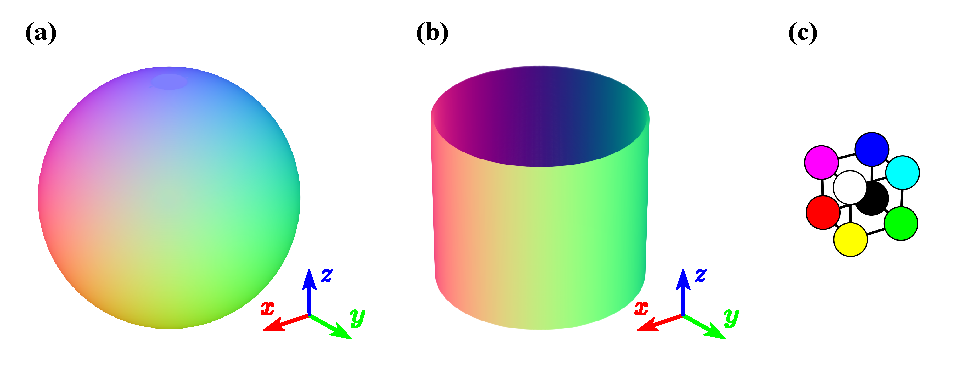
\includegraphics[width=0.96\textwidth]{artwork/normals.pdf}
    \caption{Spatial distribution of unit normal vectors on (a) the sphere, and (b) lateral surface of the cylinder, represented by red-green-blue values with respect to (c) the color cube.}
    \label{fig:normals}
\end{figure}

\subsection{Normal Estimation on Nonplanar Anatomical Surfaces}
Anatomical body models are usually created as either the computer-aided design or voxel computational models.
These models are developed upon medical scans and images to a certain level of resolution, which is dependent on the resolution of recording devices.
A very efficient representation of an anatomical model is by using the unstructured \gls{3-d} point cloud on the surface.
The surface of a model represents a compact, connected and orientable \gls{2-d} manifold embedded in $\mathbb{R}^3$.
A point cloud on the surface is represented as a collection of coordinates $\mathbb{X} = \left\{ \mathbf{x}_1, \mathbf{x}_2, \dots, \mathbf{x}_n \right\}$ where $\mathbf{x}_i = (x_i, y_i, z_i) \in \mathbb{X}, \; 1 \leq i \leq n$.

If the model itself does not contain any information on surface normals, they should be estimated at every point in the iterative manner on a local scale~\cite{Berger2017survey}.
There are several existing normal estimation techniques, each adapted according to the particular shape of the surface, noise level, the incidence of sharp edges, etc.
These techniques are broadly classified into two separate classes: ``traditional'' and learning-based normal estimation.

``Traditional'' techniques generally rely on the analysis of the covariance matrix composed from a local patch around a query point in the cloud.
Furthermore, these techniques can be divided into two additional sub-classes: optimization-based and averaging techniques~\cite{Klasing2009Comparison}.
Optimization-based techniques estimate a normal by minimizing the cost function penalizing a certain criterion, such as the distance of points to a local tangent plane or the angle between tangential vectors and the normal vector~\cite{Hoppe1992Surface}.
On the contrary, averaging techniques are calculating the normal vector as the weighted average of normal vectors on the triangles formed with pairs of neighboring points within a local patch~\cite{Jin2005comparison}.

Learning-based techniques are divided into the regression- and surface fitting-based techniques~\cite{Wang2015Designing}.
These techniques are introduced in order to solve recurrent issues in normal estimation on non-differentiable/non-smooth regions on the surface.
In addition, learning-based techniques significantly improve robustness to various noise levels and point density variations.
Regression-based techniques directly predict the direction of each normal utilizing various architectures of deep neural networks and the latest achievements in computer vision research~\cite{Charles2017PointNet,Guerrero2018PCPNet,Ben-Shabat2019Nesti-Net,Zhou2023Refine-Net}.
Surface fitting-based techniques effectively act as an extension to any ``traditional'' technique.
In most cases this involves using deep neural networks to predict the optimal set of weights either for the tangent plane fitting or extraction of the local neighborhood around a query point~\cite{Lenssen2020Deep,Ben-Shabat2020DeepFit,Zhu2021AdaFit,Li2022HSurf-Net}.

Given the anatomical models are generally free of noise and outliers, sampled densely enough, and differentiable across the entire surface, the focus in this thesis is on ``traditional'' techniques, primarily on techniques based on (weighted) moving least squares, which will be discussed in more detail later in the chapter.

A unit normal vector, $\mathbf{\hat n}$, is assigned at each point, $\mathbf{x}_i$, of the point cloud, $\mathbb{X}$.
The direction of $\mathbf{\hat n}$ is estimated by fitting a local plane and extracting its principal components.
First, $\mathbb{X}$ is organized into a \gls{k-d} tree, a space-partitioning data structure that allows searching for the nearest neighbors of a point according to a certain criterion~\cite{Bentley1975Multidimensional}.
Then, $k$ nearest neighbors around $\mathbf{x}_i$ are extracted.
The nearest neighbors represent a local patch of points, $nbhd(\mathbf{x}_i)$, from which the covariance matrix is composed.
After decomposition of the matrix by using the \gls{pca}, the eigenvector with the smallest corresponding eigenvalue is orthogonal to the tangent plane at $\mathbf{x}_i$ and thus represents the unit normal vector.
Other two eigenvectors lie in the tangent plane and represent the unit binormal, $\mathbf{\hat b}$, and unit tangent vector, $\mathbf{\hat t}$.
In the illustrative example shown in~\cref{fig:normal_estimation}, a positional relationship between principal components extracted from the covariance matrix of $nbhd(\mathbf{x}_i)$ is shown.
\begin{figure}[t]
    \centering
    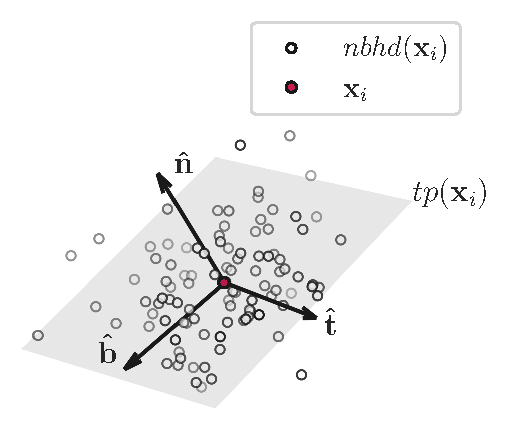
\includegraphics[width=0.46\textwidth]{artwork/normal_estimation.pdf}
    \caption{The unit binormal, tangent and normal vector at the query point with respect to the local neighborhood surrounding that point.}
    \label{fig:normal_estimation}
\end{figure}
These three orthogonal vectors $\left\{ \mathbf{\hat b}, \mathbf{\hat t}, \mathbf{\hat n} \right\}$ span $\mathbb{R}^3$ and form an orthonormal basis on a local scale with $\mathbf{x}_i$ at the origin.
This process should be repeated for each $\mathbf{x}_i$ in $\mathbb{X}$ to obtain the unit normal vector field over the entire surface.

Fitting a local tangent plane to a query point is performed as follows.
The ``centroid'' of $nbhd(\mathbf{x}_i)$ is first computed as
\begin{align}
    m_i = \frac{1}{k} \; \sum_{j=1}^{k} \mathbf{x}_j.
\end{align}
Here, $k$ stands for the number of points in $nbhd(\mathbf{x}_i)$, whereas $\mathbf{x}_j$ represents a point in $nbhd(\mathbf{x}_i)$.
A tangential plane can then be found by minimizing the Euclidean distance vector, $\mathbf{y}_j$, between each point in $nbhd(\mathbf{x}_i)$ and $\mathbf{m}_i$
\begin{align}
    \label{eqn:constrained_1}
    \min_{\left| \mathbf{n}_i \right| = 1} \sum_{j=1}^{k} \left( \mathbf{y}_j^\intercal \mathbf{n}_i \right)^2.
\end{align}
The above expression can be rewritten in matrix notation as
\begin{align}
    \label{eqn:constrained_2}
    \min_{ \mathbf{n}_i^\intercal \mathbf{n}_i = 1} \mathbf{n}_i^\intercal \left( \mathbf{Y}_i \mathbf{Y}_i^\intercal \right) \mathbf{n}_i,
\end{align}
where
\begin{align}
    \mathbf{Y}_i = \begin{pmatrix}
    \vline & \vline &  & \vline &  & \vline \\
    \mathbf{y}_1 & \mathbf{y}_2 & \dots & \mathbf{y}_j & \dots & \mathbf{y}_k \\
    \vline & \vline &  & \vline &  & \vline
    \end{pmatrix}.
\end{align}

Instead of the imposed constrained optimization in~\cref{eqn:constrained_1,eqn:constrained_2}, $f(\mathbf{n}_i) = \mathbf{n}_i^\intercal \mathbf{S}_i \mathbf{n}_i$, where $\mathbf{S}_i = \mathbf{Y}_i \mathbf{Y}_i^\intercal$, is subjected to the equality constraint, $g(\mathbf{n}_i) = \mathbf{n}_i^\intercal \mathbf{n}_i - 1$, and the Lagrangian function is constructed as
\begin{equation*}
    \mathcal{L}(\mathbf{n}_i, \lambda) = f(\mathbf{n}_i) - \lambda g(\mathbf{n}_i).
\end{equation*}
The constrained optimization is now converted into the unconstrained minimization of $\mathcal{L}(\mathbf{n}_i, \lambda)$ simply by equating the gradient of the Lagrangian to zero,
\begin{align}
    \nabla \mathcal{L}(\mathbf{n}_i, \lambda) &= 0, \\
    \frac{\partial \mathcal{L}}{\partial \mathbf{n}_i} &= 0 \Rightarrow \mathbf{S}_i \mathbf{n}_i = \lambda \mathbf{n}_i, \\
    \frac{\partial \mathcal{L}}{\partial \lambda} &= 0 \Rightarrow \mathbf{n}_i^\intercal \mathbf{n}_i = 1.
\end{align}
A (unit) normal is then captured from
\begin{align}
    \mathbf{S}_i = \mathbf{V} \begin{pmatrix}
    \lambda_1 &  &  \\
    & \ddots & \\
    & & \lambda_d
    \end{pmatrix} \boldsymbol{V}^\intercal
\end{align}
as the eigenvector with the smallest corresponding eigenvalue.

Instead of a plane, a higher-order polynomial~\cite{Levin1998approximation}, implicit B-spline~\cite{Rouhani2015Implicit} and osculating jets (truncated Taylor expansion)~\cite{Cazals2005Estimating} can be fitted to a parametric surface in orthonormal basis.   
This is particularly important when surface normals, rather than unit normals, should be determined.
In such cases, a surface (or curvature) normal is computed as
\begin{align}
    \mathbf{n} = \frac{\partial \tilde f}{\partial u} \times \frac{\partial \tilde f}{\partial v}
\end{align}
at tangential coordinates $u = v = 0$ where $\tilde{f}(u, v)$ is the fitted ``height'' function in the normal direction.

Generally, the approach in normal estimation described previously will certainly lead to inconsistent orientation of the unit normal vector field on the surface.
This is mainly due to eigenvectors being arbitrarily oriented due to the computer implantation of the numerical solver used for the eigendecomposition of the covariance matrix.
The issue of inconsistent orientation can be resolved by finding a consistent global orientation by propagation starting from a certain viewpoint.
In general, for $\mathbb{X}$ of sufficient density given that the surface is differentiable, adjacent normal vectors, $\mathbf{n}_i$ and $\mathbf{n}_j$, at any two neighboring points, $\mathbf{x}_i$ and $\mathbf{x}_j$, should point in a similar direction.
In other words, $\mathbf{n}_i \cdot \mathbf{n}_j \approx \pm 1$ if corresponding tangent planes $tp(\mathbf{x}_i)$ and $tp(\mathbf{x}_j)$ are (nearly) parallel.
If the planes are consistently oriented then $\mathbf{n}_i \cdot \mathbf{n}_j \approx 1$.
Otherwise, if $\mathbf{n}_i \cdot \mathbf{n}_j \approx -1$, either $\mathbf{n}_i$ or $\mathbf{n}_j$ must be flipped.

This approach has two main disadvantages: it fails at sharp edges and corners, and the imposed condition should hold for \emph{all} pairs of neighboring points in the point cloud.
Since anatomical tissue models do not contain sharp edges and corners, the first outlined disadvantage can be disregarded.
Furthermore, the second shortcoming can be taken care of by constructing a so called Riemann graph over the point cloud and assigning a weight to each edge based on the similarity score between the respective points' normals~\cite{Hoppe1992Surface},
\begin{align}
    w_{ij} = 1 - \left| \mathbf{n}_i \cdot \mathbf{n}_j \right|
\end{align}
This allows the construction a minimal spanning tree across which the initial normal orientation from a single point selected as the root can be efficiently propagated.
The favorable propagation is the one that follows the direction of low curvature, thereby avoiding ambiguous situations~\cite{Berger2017survey}.

In~\cref{fig:normals_ear}, the spatial distribution of surface normals on the surface of the adult ear model is shown.
This model is taken from the third published study highlighted in~\cref{sec:publication_3}.
Surface normals are first normalized to unit length and then mapped into corresponding \gls{rgb} values (the frame of reference is shown in lower right region in~\cref{fig:normals_ear}).
\begin{figure}[t]
    \centering
    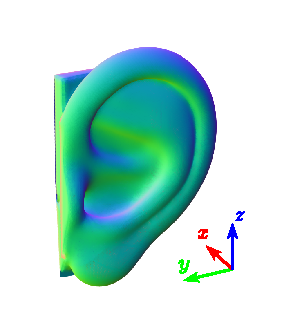
\includegraphics[width=0.4\textwidth]{artwork/normals.ear.pdf}
    \caption{Spatial distribution of normal vectors on the surface of the ear model represented by red-green-blue values.}
    \label{fig:normals_ear}
\end{figure}

\section{Construction of the Averaging Area}
\label{sec:construction_of_the_averaging_area}
The spatially averaged power density is acquired through the computation of surface integrals over the conformal averaging area, $\hat A$, on the evaluation surface.
The extent of this averaging area is contingent upon the configuration of the evaluation surface itself within the computational domain.
In the case of a nonplanar evaluation surface, the averaging area surpasses the size of its \gls{2-d} projection.
Conversely, if the evaluation surface is flat, the averaging area corresponds to the square-shape averaging area of \SIlist{4;1}{\cm\squared} as prescribed in~\cite{ICNIRP2020Guidelines,IEEE2019Standard}.

In the case of evaluation surfaces that are entirely flat, the construction of the averaging area is straightforward.
For a \SI{4}{\cm\squared} averaging area, a square shape with an edge length of \SI{2}{\cm} is employed, whereas a \SI{1}{\cm\squared} averaging area is represented by a square with an edge length of \SI{1}{\cm}~\cite{IEEE2021Guide}.
The positioning of the averaging area on the evaluation surface is determined by its center point, which corresponds to the intersection of the diagonals of the square.
To ascertain the orientation that maximizes the power passing through the averaging area, the square is rotated around its center point in increments of up to \SI{5}{\degree}~\cite{IEC63195-2-2022}.
The maximum spatially averaged power density with regards to the relative orientation at a query point is determined; further information regarding the integration of power density can be found in~\cref{sec:spatial_averaging_of_power_density}.
This process is repeated for all points on the evaluation surface.
The peak spatial-averaged power density is then reported at the point, which results in a global maximum of the spatially averaged power density.

The averaging area on the nonplanar evaluation surface is determined as the intersection with a sphere of a fixed size defined by radius $r_\text{av}$; panel \textbf{a} in~\cref{fig:evaluation_surface}.
\begin{figure}[t]
    \centering
    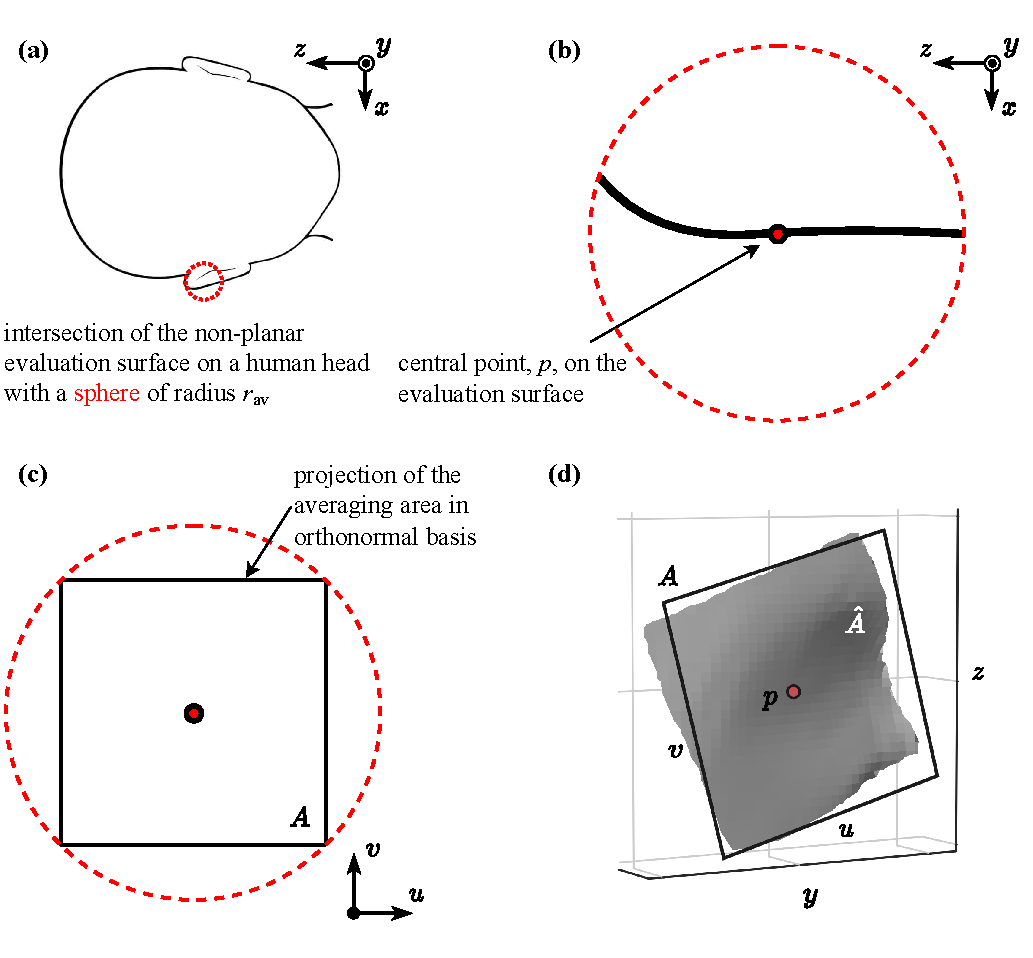
\includegraphics[width=\textwidth]{artwork/evaluation_surface.pdf}
    \caption{Construction of the averaging area on a nonplanar evaluation surface: (a) intersection of the surface of the human head with a sphere of fixed radius, (b) position of the center point of the sphere at the evaluation surface, (c) projection of the averaging area in two-dimensional space, (d) spatial relationship between the conformal averaging area and its projection.}
    \label{fig:evaluation_surface}
\end{figure}
Contrary to recommendations in~\cite{IEC63195-2-2022}, the radius is here defined as
\begin{align}
    r_\text{av} = \frac{\sqrt{2 A}}{2},
\end{align}
where $A$ is the square-shape flat averaging area.
Thus, $r_\text{av}$ corresponds to the radius of the circumscribed circle of the square-shape averaging area.
In general, a circumscribed circle (circumcircle) of a polygon is a circle that passes through all the vertices of that polygon.
The center point of a sphere is a point on the evaluation surface, shown in panel \textbf{b} in~\cref{fig:evaluation_surface}.

The averaging area is then reduced to match square shape in an orthonormal basis as follows.
First, a local patch of points contained in the intersected region is centered at zero-mean by computing the average of $x$, $y$ and $z$ coordinates and subtracting it from each point.
Subsequently, the covariance matrix is computed based on these centered coordinates.
The eigenvectors associated with the two largest eigenvalues are then identified as they represent the primary directions of variance in the spatial distribution of coordinates when projected in \gls{2-d} space.
These selected eigenvectors serve as the columns of a transformation matrix.
By multiplying the centered point cloud with this transformation matrix, it is effectively represented in \gls{2-d} space defined by parametric coordinates $u$ and $v$.
Finally, the resulting projection is constrained to match the shape and dimensions of the square-shape averaging area, $A$, of \SIlist{4;1}{\cm\squared}, as illustrated in panel \textbf{c} in~\cref{fig:evaluation_surface}.

Once the square-shape projection is transformed back into standard basis, the conformal averaging area, $\hat A$, is obtained (panel \textbf{d} in~\cref{fig:evaluation_surface}).
Due to the nonplanar shape of the evaluation surface, the area $\hat A$ is greater than $A$.
This deviation in size is influenced by the degree of curvature present on the evaluation surface, adhering to the principle: the greater the curvature, the greater the overall difference.
Nonetheless, by transforming the original intersection into \gls{2-d} space defined by its principal components, it is ensured that this deviation is minimized.

The method of assessment of the conformal averaging area depends on the surface discretization within the computational domain.
For example, if the evaluation surface is discretized by using triangle mesh, the standardized algorithm for area estimation exists~\cite{IEC63195-2-2022}:
\begin{itemize}
    \item specify an empty list of triangles;
    \item determine the triangles on the evaluation surface that are completely enclosed within a region of the bounded conformal averaging area;
    \item append the encompassed triangles to the list of triangles specified in the first step that are connected to the triangles that contain the center point via other triangles that are located completely inside a region of the bounded conformal averaging area;
    \item determine the triangles that intersect the surface of the sphere and the intersection points of their edges with the averaging surface; determine the triangles specified by these intersection points and the corner points of the triangles of the evaluation surface; if the geometric centers of the triangles are inside the averaging surface, add the triangles to the list;
    \item sum the areas of all triangles contained in the list.
\end{itemize}

Alternatively, when solely the spatial distribution of unstructured points sampled on the surface is available, without any information about the positional relationship between the points, the conformal averaging area can be estimated by approximating the surface integral of the magnitude of the surface normal vector field.
The surface integral is precisely defined within the bounds of the parameters. 
These parameter bounds are determined to represent the surface as a graph of a bi-variate ``height'' function, relative to the $z$-direction aligned with the unit normal at the center point on that surface.
This approach guarantees the square shape of the integration domain and the magnitude of surface normals is represented as the scalar field on this integration domain as
\begin{align}
    \left| \mathbf{\tilde n} \right| = f(x, y).
\end{align}
The integral can be approximated by any accurate \gls{2-d} quadrature technique.
One approach is to fit the scalar field by a smooth bi-variate spline constructed as tensor products of \gls{1-d} splines to satisfy
\begin{align}
    \sum_{i} \left[ w_i \left( f(x_i, y_i) - \left| \mathbf{n}_i \right| \right) \right]^2 \leq s,
\end{align}
where $w_i$ are non-negative weights, and $s$ is the smoothing factor, which controls the smoothness of the resulting function $f(x, y)$ and the overall accuracy of the approximation. 
\Gls{1-d} splines are defined by the specific polynomial degree separately in $x$- and $y$-direction.
Generally, for data sampled densely enough, a bi-cubic spline is a natural choice.
As the integral of a bi-cubic spline can be calculated analytically, the surface integral of $f(x, y)$ is determined as the incremental sum of contributions of individual splines within the integration domain on which $f(x, y)$ is defined.

\section{Spatial Averaging of Power Density}
\label{sec:spatial_averaging_of_power_density}
In practical applications, compliance with the current exposure limits at \SIrange{6}{300}{\GHz} involves the computation of spatially averaged \gls{ipd}.
The spatially averaged \gls{ipd} on the surface of the exposed tissue is subject to various specifications, which depend on the prevailing incidence direction and polarization of the \gls{emf}~\cite{IEC63195-2-2022}.
The integrand functions corresponding to these specification are multiplied by additional functions that account for the angle between the Poynting vector and surface normals.
This ensures that contributions from regions where the Poynting vector points outward from the evaluation surface or is parallel to the tangential plane at a specific point on the surface are not considered in computation.

The first specification pertains to the power density of the surface-normal propagation direction into the evaluation surface.
The computation of the spatially averaged power density at a specific location, as determined by the position vector, $\mathbf{r}_0$, follows the expression presented below~\cite{IEC63195-2-2022}:
\begin{align}
    \label{eqn:propagation-direction}
    S_\text{inc, n}(\mathbf{r}_0) = \frac{1}{2 \hat{A}\left( \mathbf{r}_0 \right)} \; \iint_{A \left( \mathbf{r}_0 \right)} \Theta \left\{ \Re \left[ \mathbf{E \left( r \right)} \times \mathbf{H^* \left( r \right)} \right] \cdot \mathbf{\hat{n} \left( r \right)} \right\} \cdot \Re \left[ \mathbf{E \left( r \right)} \times \mathbf{H^* \left( r \right)} \right] \cdot \mathbf{\hat{n} \left( r \right)} \; \mathrm{d}\hat{A}\left( \mathbf{r} \right).
\end{align}
In this equation, the Heaviside function, $\Theta(\cdot)$, assumes a crucial role.
This function ensures that the integrand function is zero if the angle between the Poynting vector and a normal vector (which is assumed to point into the irradiated solid volume bounded by the surface) is within the \SIrange{90}{270}{\degree} range.
This adjustment is necessary to account for situations where the normal component of the Poynting vector would otherwise yield a negative value.
Additionally, within the equation, $\hat A$ stands for the conformal averaging area, with $\hat A$ being always greater than $A$ for nonplanar surfaces.
The positional vector, denoted as $\mathbf{r}$, refers to a point on the surface determined by the area $\hat A$.

Additionally, the total propagating power density into the evaluation surface, is defined in~\cite{IEC63195-1-2022,IEC63195-2-2022} as
\begin{align}
    \label{eqn:total}
    S_\text{inc, tot}(\mathbf{r}_0) = \frac{1}{2 \hat{A}(\mathbf{r}_0)} \iint_{A(\mathbf{r}_0)} \left\| \Re \left[ \mathbf{E}(\mathbf{r}) \times \mathbf{H}^*(\mathbf{r}) \right] \right\| \cdot \Xi \left( \delta \right) \; \mathrm{d}\hat{A}(\mathbf{r}),
\end{align}
where
\begin{align}
    \delta = \cos^{-1}\left[ {\frac{\Re \left[ \mathbf{E}(\mathbf{r}) \times \mathbf{H}(\mathbf{r})^* \right]}{\left\| \Re \left[ \mathbf{E}(\mathbf{r}) \times \mathbf{H}(\mathbf{r})^* \right] \right\|} \cdot \mathbf{n}(\mathbf{r})} \right],
\end{align}
and
\begin{align}
\Xi(\delta) = \begin{cases}
        1, & \text{if } \SI{0}{\degree} \leq \delta < \SI{85}{\degree} \\
        1 - \nicefrac{(\delta - \SI{85}{\degree})}{\SI{5}{\degree}}, & \text{if } \SI{85}{\degree} \leq \delta < \SI{90}{\degree} \\
        0, & \text{otherwise}.
    \end{cases}
\end{align}

The final aspect to note is the exclusion of the discussion on the total power density directed into the exposed model in the context of near-field exposure.
Specifically, in the reactive near field, the prevailing influence stems from the non-propagating energy encapsulated within the imaginary component of the Poynting vector.
Consequently, the magnitude of the imaginary part should be incorporated into the spatial averaging procedure.
However, it is important to highlight that both the \gls{icnirp} guidelines~\cite{ICNIRP2020Guidelines} and \gls{ieee} standard~\cite{IEEE2019Standard} advise against assessment of the spatially averaged \gls{ipd} in the reactive near field.
Instead, in this region, the determination of \gls{br}s is recommended as the appropriate approach.

Any accurate \gls{2-d} quadrature technique may be employed in order to solve for surface integrals specified in~\cref{eqn:propagation-direction,eqn:total}.
In most cases, the choice of the quadrature method depends on the interpolation approach adopted for the integrand function.
In general, the Gauss-Kronrod quadrature formula, can be utilized regardless of the interpolation method employed.
This adaptive numerical integration method is based on Gaussian quadrature, with evaluation points selected strategically to ensure an accurate approximation by utilizing information obtained from computations of less accurate approximations.
Furthermore, this method eliminates the need for explicitly defining the degree of quadrature.
A typical choice combines a \num{7}-point Gauss rule with a \num{15}-point Kronrod rule~\cite{Kahaner1989Numerical}.
However, it is important to note that the Gauss-Kronrod quadrature can be computationally intensive, particularly when a large number of surface integrals needs to be evaluated, depending on the complexity of the integrand function.
A detailed discussion on the selection of the quadrature technique can be found in the fourth published paper in~\cref{sec:publication_4}.

The automatic detection of the region of highest exposure involves a set of sequential steps, as outlined below:
\begin{itemize}
    \item assuming a nonplanar model is represented by an oriented set of points $\mathbb{X} = \{ \mathbf{x}_1, \mathbf{x}_2, \dots, \mathbf{x}_n \} \subset \mathbb{R}^3$, organize it into a \gls{3-d} \gls{k-d} tree;
    \item identify points visible from the predefined direction~\cite{Katz2007Direct}, which should correspond to the propagation direction of the \gls{emf}; this step is optional, but it allows to focus solely on a region that is in the line of sight of \gls{emf} sources;
    \item for each point (in the visible subset of points), extract the local neighborhood by considering points located within a sphere of a radius $\nicefrac{\sqrt{2 A}}{2}$, where $A$ represents the size of the square integration domain;
    \item perform a change of basis on the local neighborhood using the \gls{pca}, which leads to the alignment of the tangential principal components with $A$;
    \item compute the area of a conformal averaging area, $\hat A$, by approximating the surface integral of the magnitude of surface normals on the corresponding surface;
    \item compute the spatially averaged power density using the approach outlined in~\cref{eqn:propagation-direction,eqn:total}.
\end{itemize} 

To demonstrate the practical application of the automated detection, we consider the realistic human head model\footnote{Courtesy of H. Dodig, University of Split, Faculty of Maritime Studies} exposed to \gls{rf} energy in a Gaussian pattern~\cite{Foster2016Thermal} (approximating the exposure conditions in~\cite{Colombi2015Implications}).
The original \gls{3-d} model is constructed from magnetic resonance imaging scans of a \num{24}-year-old male volunteer~\cite{Laakso2015Intersubject}.
However, in this illustration, we represent the input model as an unstructured point cloud comprising \num{63333} surface points.
The reconstructed surface of the point cloud model, obtained using the Poisson method~\cite{Kazhdan2006Poisson}, which solves for an approximate indicator function matching the input normals' gradient, is depicted in panel \textbf{a} in~\cref{fig:head}.

The estimation of surface normals is carried out by using the weighted least squares method~\cite{Levin1998approximation}, as outlined in the preceding section.
The spatial distribution of unit normals on the surface of the head model is visualized in panel \textbf{b} in~\cref{fig:head}, using the \gls{rgb} representation.
It is important to note that the surface normals are shown pointing outward from the volume enclosed by the surface.
However, during subsequent spatial averaging of the power density, the normals are assumed to point inward to align with the direction of incidence of the \gls{emf}, thereby avoiding any physical inconsistencies.

The power density incident on the surface of the human head follows a Gaussian pattern, depicted in panel \textbf{c} in~\cref{fig:head} and mathematically represented by the following expression:
\begin{align}
    S_\text{inc}(x, y, z) = I_0 \; e^{-\left( \nicefrac{d}{\rho} \right)^2}.
\end{align}
In the equation, $I_0$ represents the peak \gls{ipd} of \SI{10}{\watt\per\m\squared}, located at the point closest to the theoretical radiation source with respect to the $x$-axis in the upper crus region of the antihelix on the right outer ear.
The scaled Euclidean distance, here denoted by $d$, measures the distance between the point of the peak \gls{ipd}, $(x_c, y_c, z_c)$, and a point on the evaluation surface, $(x, y, z)$.
The original Euclidean distance is additionally scaled to deform the otherwise circular pattern into an elliptical shape as
\begin{align}
    d = d(x, y, z) = \sqrt{\left( \frac{(x - x_c)^2}{s_x} + \frac{(y - y_c)^2}{s_y} + \frac{(z - z_c)^2}{s_z} \right)},
\end{align}
where  $s_x$, $s_y$ and $s_z$ correspond to \num{1}, \num{0.5} and \num{0.25}, respectively.
The scaled distance is bounded within the radius of ``influence'', $\rho$, set to \SI{2.5}{\cm} in this particular case.

Finally, panel \textbf{d} in~\cref{fig:head} shows the square projection of the conformal averaging area corresponding to the most exposed region on the evaluation surface.
Before executing the algorithm for automated detection of the peak spatial-averaged power density, the surface is resampled into a point cloud where only the points directly visible from the perspective of the \gls{emf} incidence point of view (in the negative $x$-direction) are considered.
The hidden point removal operator~\cite{Katz2007Direct}, which determines the visible points in a point cloud, as viewed from any given viewpoint is employed.
The spatial averaging of the power density within this region of the surface yields a value of \SI{4.45}{\watt\per\m\squared}.
\begin{figure}[t]
    \centering
    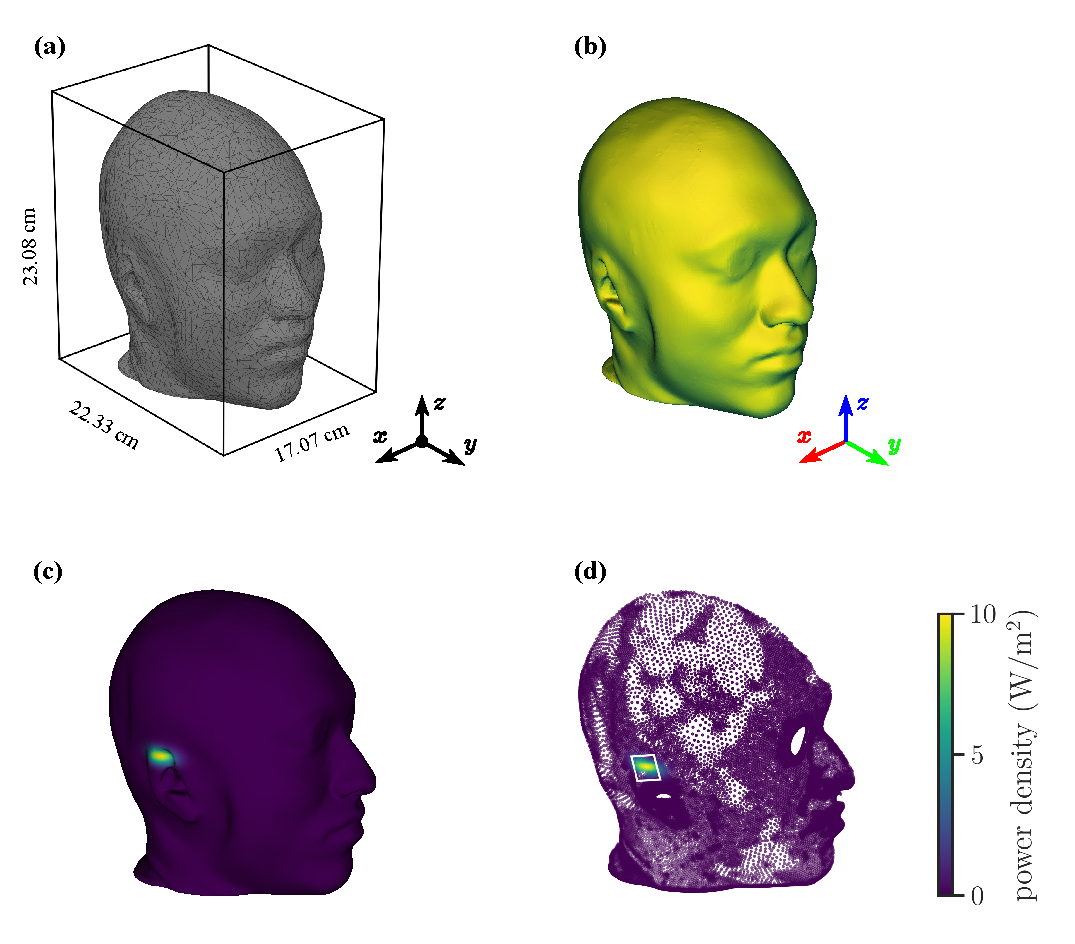
\includegraphics[width=\textwidth]{artwork/head.pdf}
    \caption{Spatial averaging of the power density on the human head model: (a) reconstructed surface of the human head, (b) unit normals directed outward from the surface (represented using red-green-blue values), (c) distribution of the power density in a Gaussian pattern with the peak value located in the upper crus of the right antihelix, (d) position of the square projection of the conformal averaging region on the surface where the spatial averaging of the power density results in a global maximum value.}
    \label{fig:head} 
\end{figure}

    \cleardoublepage

\chapter{PUBLISHED PAPERS}
\label{chap:5}
In this chapter, the abstracts of published papers forming the basis of the thesis are outlined.
Along with the abstracts, an impact statement and/or graphical summary is given, demonstrating the scientific contribution of each paper.
Additionally, the contribution of individual researchers---authors of a particular paper---is indicated by using ``Contributor Roles Taxonomy'' or CRediT for short.
CRediT is a high-level taxonomy able to represent the roles of contributors to research outputs~\cite{Allen2014CRediT}.
It has proven to be an effective means of documenting ``Who Did What?'', which is unattainable by observing the positions within the author list alone~\cite{Holcombe2020tenzing}.
There are in total fourteen contributor roles described briefly below~\cite{CRT2023Roles}:
\begin{description}[leftmargin=!,labelwidth=\widthof{\bfseries Writing -- Review and editing}]
    \item[Conceptualization] formulation of overarching research goals and aims of the study
    \item[Data curation] production of metadata, maintaining the research data (including software code, if applicable) for initial use and later re-use to support reproducibility~\cite{Stodden2016Reproducibility}
    \item[Formal analysis] application of statistical, mathematical, computational, or other formal techniques to analyze and/or synthesize data
    \item[Funding acquisition] acquisition of the financial support for the project
    \item[Investigation] a research and investigation process, i.e., performing the experiments and/or data collection
    \item[Methodology] development of the models
    \item[Project administration] management and coordination responsibility for the research activity planning and execution
    \item[Resources] provision of study materials, reagents, materials, patients, laboratory samples, animals, instrumentation, computing resources, or other analysis tools
    \item[Software] development of computer programs which includes, but is not limited to the implementation of the computer code and supporting algorithms, testing the code, and further deploying and adjusting of the existing code base
    \item[Supervision] oversight and leadership responsibility for the research planning and execution
    \item[Validation] ensuring the models correspond to the specification defined during the \textbf{Conceptualization} phase; additional verification of the reproducibility of all research outputs
    \item[Visualization] preparation, creation and/or presentation of the published work, specifically visualization/data presentation
    \item[Writing -- Original draft] preparation, creation and/or presentation of the published work in its initial version
    \item[Writing -- Review and editing] critical review, commentary or revision during review (if applicable) and post-publication
\end{description}

\section{Assessment of Incident Power Density on Spherical Head Model up to 100 GHz}
\label{sec:publication_1}
\subsection{Abstract}
This article presents a technique for the accurate assessment of the spatially averaged incident power density (IPD) on a spherical human head model from 3.5 to 100 GHz.
The spatially-averaged IPD is defined either by averaging components of the power density vector normal to an evaluation surface, or by averaging its norm.
The electromagnetic exposure assessment is provided for a dipole antenna placed at a separation distance of 2--150 mm from the model.
We compare the IPD averaged over a proposed spherical surface with differently positioned planar surfaces.
Results show that, for appropriate settings of the exposure above 6 GHz, the IPD averaged on a spherical surface is up to 12\% larger for the normal definition, while marginally lower for the norm definition.
In the worst case scenario, the spatially averaged IPD on a spherical surface is up to about 30\% larger regardless of the definition.
Comparative analysis between the definitions of the IPD averaged on a spherical model demonstrates that the norm definition yields significantly larger values in the reactive near field at characteristic frequencies, whereby this difference is marginal out of the reactive near field.

\subsection{Impact Statement}
This article introduces an accurate method for the assessment of the spatially averaged \gls{ipd} on a surface of the spherical human head model.
Both definitions of the spatially averaged \gls{ipd}, described in previous chapters and in the paper itself, available in~\cref{chap:a}, have been used to validate the proposed approach.
This approach itself allows for a more sophisticated exposure assessment as the evaluation surface is nonplanar.

Experiments have been done at the \SIrange{3.5}{100}{\GHz} range for the antenna-to-head separation distance of \SIrange{2}{150}{\mm}.
The antenna is modelled as the half-wavelength dipole driven at its center by a voltage source set to \SI{1}{V}.
Spatial averaging is performed by following the latest specification given in the \gls{icnirp} guidelines~\cite{ICNIRP2020Guidelines} and \gls{ieee} standard~\cite{IEEE2019Standard}.

Computational results indicate substantial differences between \gls{ipd} averaged on the spherical and flat evaluation surface.
Namely, in the worst case exposure scenario, relative differences are \SIlist{28.35;31.31}{\percent} for different definitions of the spatially averaged \gls{ipd}, i.e., by taking into account the normal components and  magnitude of the real part of the power density vector field, respectively.
This difference is less pronounced (\SI{11.11}{\percent} in the worst case) for more appropriate exposure settings, i.e., in comparison with the flat surface that lies on a tangent plane to a spherical averaging surface in the nearest point relative to the antenna.
Comparative analysis between definitions of the spatially averaged \gls{ipd} on the spherical model have shown substantial differences in the reactive near field, which is especially emphasized at lower frequencies.

The level of curvature of the spherical evaluation surface above \SI{6}{\GHz} has been shown to be positively correlated with the value of the spatially averaged \gls{ipd}.
This implies that the use of flat evaluation surfaces eventually leads to underestimation of the spatially averaged dosimetric values and confirms the assumption that even canonical nonplanar models, such as the sphere, are better suited for practical compliance assessment of exposure of nonplanar body parts.

\subsection{Author Contributions}
Authors: Ante Kapetanović and Dragan Poljak.\\
Conceptualization: AK and DP; data curation: AK; formal analysis: AK; funding acquisition: DP; investigation: AK; methodology: AK; project administration: AK and DP; software: AK; supervision: DP; validation: AK and DP; visualization: AK; writing -- original draft: AK; writing -- review and editing: AK and DP.

\subsection{Supplementary Materials}
Data and code are available on GitHub: \url{https://github.com/akapet00/EMF-exposure-analysis/tree/main/playground/IEEE-TEMC_paper}.

\section{Machine Learning-Assisted Antenna Modelling for Realistic Assessment of Incident Power Density on Nonplanar Surfaces above \SI{6}{\GHz}}
\label{sec:publication_2}
\subsection{Abstract}
In this paper, the analysis of exposure reference levels is performed for the case of a half-wavelength dipole antenna positioned in the immediate vicinity of non-planar body parts.
The incident power density (IPD) spatially averaged over the spherical and cylindrical surface is computed at the 6–90 GHz range, and subsequently placed in the context of the current international guidelines and standards for limiting exposure to electromagnetic (EM) fields which are defined considering planar computational tissue models.
As numerical errors are ubiquitous at such high frequencies, the spatial resolution of EM models needs to be increased which in turn results in increased computational complexity and memory requirements.
To alleviate this issue, we hybridise machine learning and traditional scientific computing approaches through differentiable programming paradigm.
Findings demonstrate a strong positive effect the curvature of non-planar models has on the spatially averaged IPD with up to 15\% larger values compared to the corresponding planar model in considered exposure scenarios.

\subsection{Impact Statement}
In addition to the spherical model, this paper introduces a technique for the assessment of the spatially averaged \gls{ipd} on a surface of the cylindrical model.
As it has been previously demonstrated in~\cref{sec:publication_1}, the distribution of normal vectors on the nonplanar evaluation surface significantly affects the value of the spatially averaged \gls{ipd} computed by averaging the normal components of the real part of the power density vector field.
Contrary, it has been assumed that the spatially averaged \gls{ipd} computed by averaging the magnitude of the real part of the power density vector field will result in the same values regardless of the geometry of an exposed surface.
With this approach, the exposure of nonplanar body parts, such as fingers (along with the ear and head, the most exposed part of the body during a practical exposure scenario) can be accurately assessed.

As a proof of concept, both the spherical and cylindrical model for various curvature radii within the \SIrange{5}{15}{\cm} range have been irradiated by a half-wavelength dipole antenna operating at \SIrange{6}{90}{\GHz}.
To put them in the frame of reference, results from nonplanar models have been compared with the flat model positioned tangentially at the closest point(s) of either nonplanar model relative to the antenna.
Spatial averaging has been performed on a square \SI{4}{\cm\squared} area at \SIrange{6}{30}{\GHz} and \SI{1}{\cm\squared} above \SI{30}{\GHz} to account for the focused beams~\cite{Hashimoto2017averaging,Foster2016Thermal}.
Additionally, the computational model of the antenna have been aided with machine learning to alleviate the numerical errors ubiquitous at high-frequency \gls{emf} simulations.

Results indicate that the curvature of the nonplanar evaluation surface strongly affects the overall spatially averaged \gls{ipd}.
Unlike on spherical, the spatially averaged \gls{ipd} on cylindrical models is only slightly larger (up to \SI{4.4}{\percent} in the studied experiments) compared to the traditional flat model.
This phenomenon can most likely be explained by the spatial arrangement of the normal vectors on the surface.
Namely, spatial averaging on a flat surface is performed by integrating contributions of the power density considering only a single component of the vector field normal to the surface.
Spatial averaging on nonplanar surfaces must be performed including all components of the normal vector field.
However, the spatial distribution of normals on the surface of the cylindrical model is closer to that of the flat model as the curvature along its central axis is zero.
Thereby, only two spatial components of the parametric representation of the cylindrical evaluation surface are considered, whereas, in the case of the spherical model, all three components contribute to the curvature.

Overall this paper offers provides confirmation of the following assumptions presented in~\cref{chap:1}:
\begin{itemize}
    \item cylindrical models are better suited for practical compliance assessment in comparison to flat models;
    \item spatial distribution of normals has a strong impact on the averaging of the surface-normal propagation-direction power density into the nonplanar evaluation surface;
    \item hybridization of machine learning and traditional numerical methods through the framework of differentiable programming facilitates \gls{emf}-exposure modeling and allows high-fidelity simulations.
\end{itemize}

\subsection{Author Contributions}
Authors: Ante Kapetanović and Dragan Poljak.\\
Conceptualization: AK and DP; data curation: AK; formal analysis: AK; funding acquisition: DP; investigation: AK; methodology: AK; project administration: AK and DP; software: AK; supervision: DP; validation: AK and DP; visualization: AK; writing -- original draft: AK; writing -- review and editing: AK and DP.

\subsection{Supplementary Materials}
Data and code are available on GitHub: \url{https://github.com/akapet00/EMF-exposure-analysis/tree/main/playground/IRPA2022_paper}.

\section{Area-Averaged Transmitted and Absorbed Power Density on a Realistic Ear Model}
\label{sec:publication_3}
\subsection{Abstract}
At millimeter waves (MMW), the current state of research in computational dosimetry is mainly relying on flat-surface tissue-equivalent models to simplify the exposure assessment by disregarding geometrical irregularities characteristic of conformal surfaces on realistic models.
However, this can lead to errors in estimation of dosimetric quantities on non-planar body parts with local curvature radii comparable to the wavelength of the incident field.
In this study, we address this problem by developing an averaging technique for the assessment of the absorbed power density ($S_\text{ab}$) on the anatomically-accurate electromagnetic (EM) model of the human ear.
The dosimetric analysis is performed for the plane-wave exposure at 26 and 60 GHz, and the accuracy of the proposed method is verified by using two commercial EM software. Furthermore, we compare the two definitions of $S_\text{ab}$ provided in the international guidelines and standards for limiting exposure to EM fields above 6 GHz.
Results show marginal relative differences between the obtained values from the two different definitions (within about 6\%) in all considered scenarios.
On the other hand, in comparison to flat models, the spatial maximum $S_\text{ab}$ on the ear is up to about 20\% larger regardless of definition.
These findings demonstrate a promising potential of the proposed method for the assessment of $S_\text{ab}$ on surfaces of anatomical models at frequencies upcoming for the 5th generation (5G) wireless networks and beyond.

\subsection{Impact Statement}
This study presents a novel numerical technique for the extraction of the spatially averaged \gls{apd} on the conformal evaluation surface on a realistic tissue-equivalent electromagnetic model to accurately assess exposure above \SI{6}{\GHz}.

In~\cref{fig:Kapetanovic2022JERM}, the overview of the assessment process is shown.
In panel \textbf{a}, the computational model on the adult ear used in experiments is shown.
Furthermore, panel \textbf{b} depicts the relationship between the conformal evaluation surface and its projection positioned perpendicular to the plane wave incidence point of view in \gls{2-d} space.
Panel \textbf{c} represents the spatial distribution of the power density flux through the entire irradiated surface, where the white square emphasizes the ``hot-spot'' region, that is, the surface which yields the peak spatial-averaged \gls{apd}.
In panel \textbf{d}, the discrepancy between the transmitted and absorbed power distributed on the ``hot-spot'' region is shown.
Finally, panel \textbf{e} summarizes collected results.
\begin{figure}[ht]
    \begin{center}  
    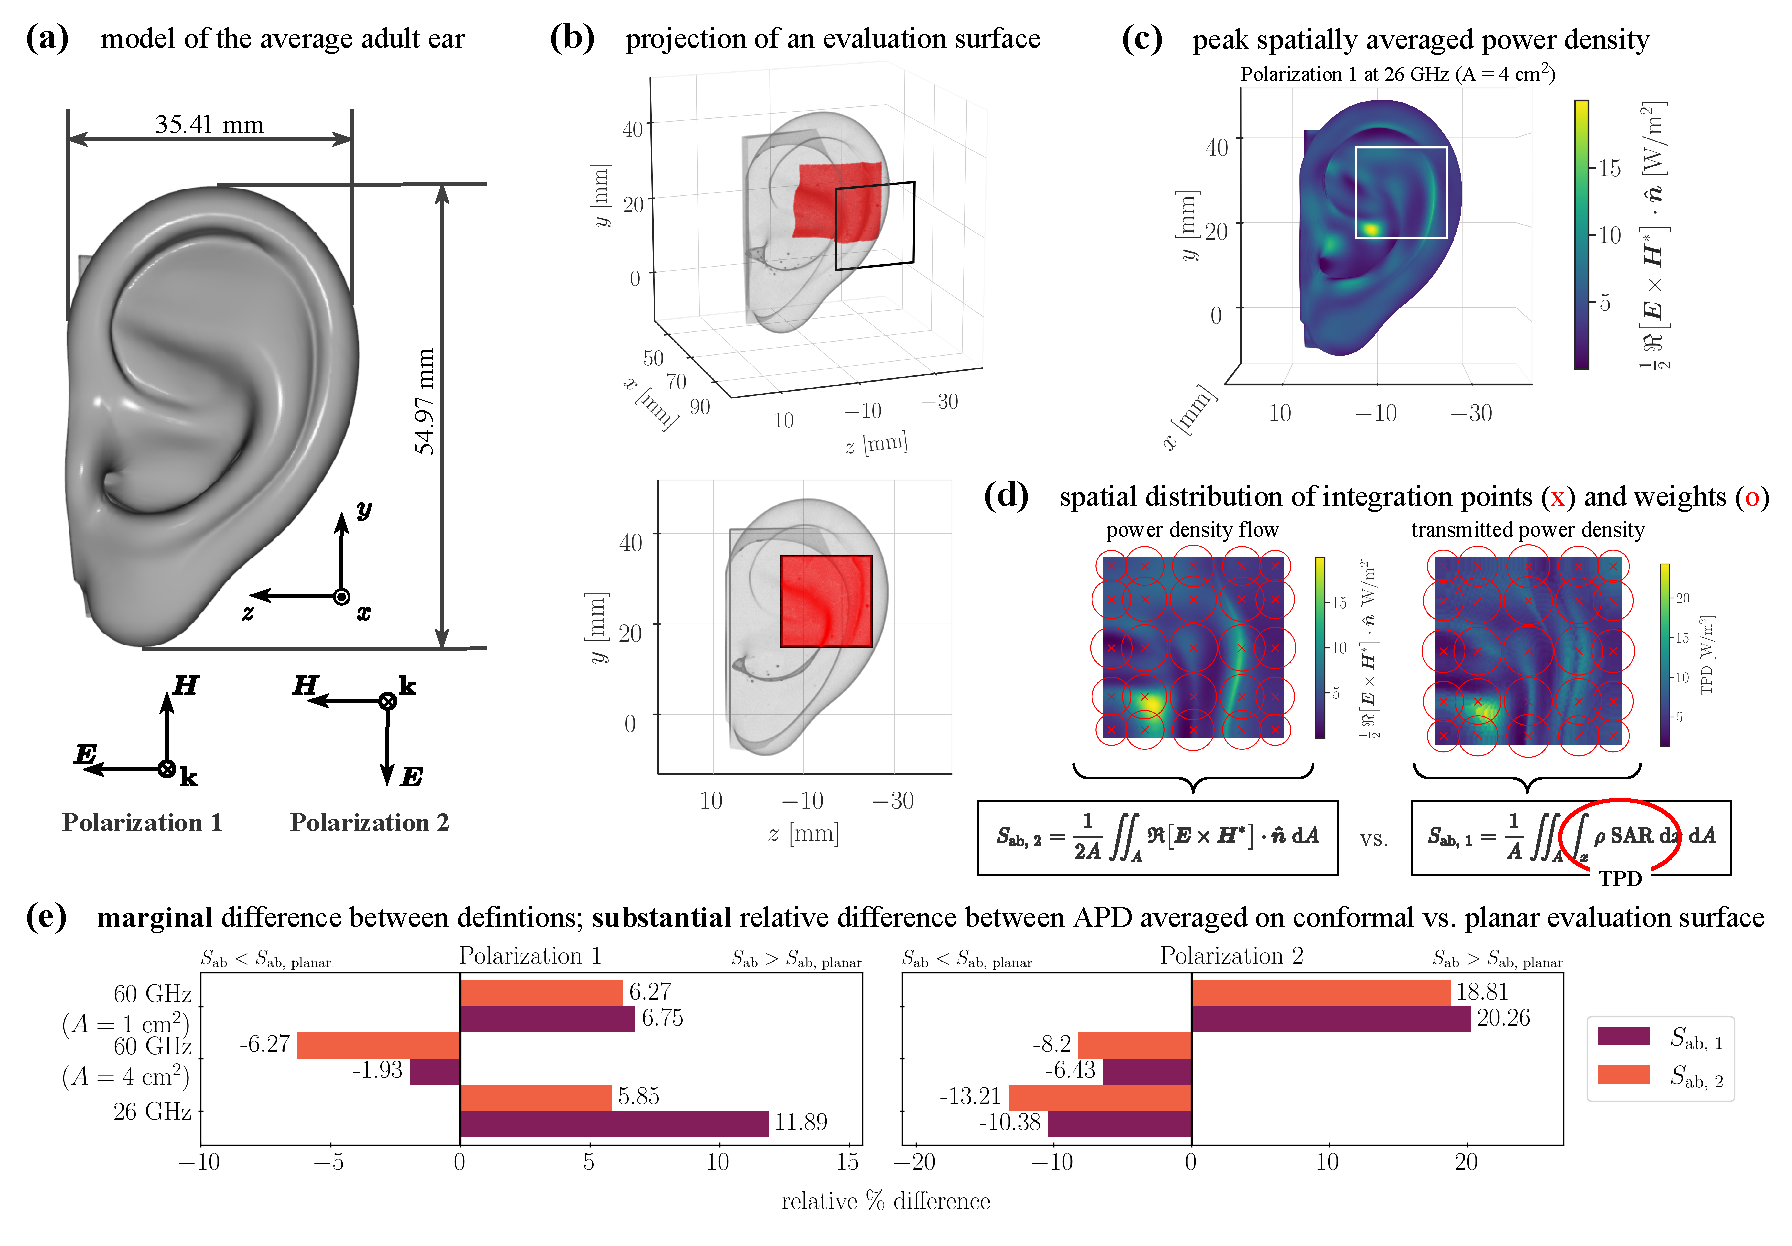
\includegraphics[width=\textwidth]{artwork/Kapetanovic2022JERM.pdf}
    \caption{Overview of the assessment process and quantitative comparison of the peak absorbed power density spatially averaged on the conformal evaluation surface of the average adult ear model by using the volumetric and surface definition.}
    \label{fig:Kapetanovic2022JERM}
    \end{center}
\end{figure}

The analysis presented in the study is focused on quantifying the superficial exposure of the human ear as it is among the most irradiated body parts in common exposure scenarios in terms of two different definitions of the spatially averaged \gls{apd} at \SIlist{26;60}{\GHz} -- frequencies upcoming for the \gls{5g} standard for broadband cellular networks.
The findings demonstrate a strong effect of irregularities in the geometry of the averaging surface, e.g., curvature (either convex or concave), sharp edges, deformities, etc., on the spatial distribution of \gls{em} power and the spatially averaged dosimetric quantities, whose accuracy is of utmost importance especially at \gls{mmw}.
It is shown that the spatially averaged \gls{apd} is up to \SI{20}{\percent} greater on conformal surfaces where morphological features of the average human ear are considered.
Additionally, it has been confirmed that only marginal differences (up to \SI{6}{\percent} relative difference) exist between the volumetric and surface definition of the spatially averaged \gls{apd}.
This is due to shallow depth of penetration of \gls{emf} into the tissue at considered frequencies (up to \SI{1}{\mm} at \SI{26}{\GHz} and only up to about \SI{0.5}{\mm} at \SI{90}{\GHz} assuming dielectric properties of dry skin~\cite{Sasaki2017Monte}).

\subsection{Author Contributions}
Authors: Ante Kapetanović, Giulia Sacco, Dragan Poljak, and Maxim Zhadobov.\\
Conceptualization: AK, GS and MZ; data curation: AK and GS; formal analysis: AK and GS; funding acquisition: DP and MZ; investigation: AK; methodology: AK; project administration: AK, GS, DP and MZ; software: AK and GS; supervision: DP and MZ, validation: AK and GS; visualization: AK; writing -- original draft: AK and GS; writing -- review and editing: AK, GS, DP and MZ.

\subsection{Supplementary Materials}
Data and code are available on GitHub: \url{https://github.com/akapet00/EMF-exposure-analysis/tree/main/playground/IEEE-J-ERM_paper}.


\section{On the Applicability of Numerical Quadrature for Double Surface Integrals at 5G Frequencies}
\label{sec:publication_4}
\subsection{Abstract}
The human exposure assessment to wireless communications systems including the fifth generation (5G) mobile systems is related to determining the specific absorption rate (SAR) or the absorbed power density (APD).
The assessment of both quantities requires the use of various numerical techniques, including moments method (MoM).
As the use of MoM results in a fully populated system matrix, a tremendous computational cost is incurred, both in terms of matrix fill time and memory allocation, as the matrix size is directly related to frequency of the problem.
This paper investigates the applicability of numerical integration at frequencies related to 5G.
The novelty of this work is related to the comprehensive set of tests of various combination of source and observation triangles using the developed unit cube test.
A number of convergence tests were performed to investigate the effects of the increasing frequency and the discretization scheme on the numerical solution, as well as to determine how to curb the computational requirements by the proficient use of numerical integration.
The results show that in the lower gigahertz range, lower integration orders could be used, resulting in the decrease of matrix fill time without loss of solution accuracy.

\subsection{Impact Statement}
In all three previously outlined publications, surface integrals of the scalar and vector field have been approximated by using the \gls{2-d} $n$-degree Gauss-Legendre quadrature~\cite{Abramowitz1972Handbook} or the adaptive Gauss-Kronrod quadrature~\cite{Piessens1983Quadpack} depending on whether the integrands are ``well behaved'' or not.
Since ``behavior'' in this sense is a vaguely defined term as there is no strict mathematical definition for it, please refer to~\cite{Weisstein2023Pathological} for further explanation.
However, in neither publication, the reasoning for the choice of the specific quadrature scheme have been provided.

As the exposure assessment and dosimetry analysis relies on the use of sophisticated computational methods that require the iterative approximation of double surface integrals, the number of which is directly proportional to the operating frequency dictating the resolution of the \gls{em} model, it is of utmost importance to avoid the use of the quadrature degree greater than necessary to avoid increased computational cost.
The method of moments is used in this paper, which, although accurate for integral equation-based \gls{em} formulations, require fully populated system matrix whose size is related to the frequency of the problem.
This leads to the tremendous computational costs by means of the matrix fill time and corresponding memory allocation~\cite{Poljak2018conformal}.

In this paper, representing the direct extension to~\cite{Cvetkovic2021Study}, a comprehensive set of convergence tests for quadrature related to double surface integrals at frequencies related to \gls{5g} is demonstrated.
Specifically, examination on various combination of source and observation triangles has been performed.
Computational results demonstrate that the numerical solution at frequencies in the high-gigahertz range require the use of high quadrature orders as well as finer discretization schemes, resulting in significantly increased requirements for matrix storage as well as matrix fill time.
On the other hand, at low-gigahertz range by using an appropriate discretization scheme, lower integration orders could be used.
This leads to the decrease of matrix fill time without sacrificing the accuracy of the solution.

\subsection{Author Contributions}
Authors: Mario Cvetković, Dragan Poljak, Ante Kapetanović, and Hrvoje Dodig.\\
Conceptualization: MC and DP; data curation: MC; formal analysis: MC; funding acquisition: not applicable; investigation: MC, AK and HD; methodology: MC; project administration: MC, DP, AK and HD; software: MC; supervision: DP, validation: MC and AK; visualization: MC; writing -- original draft: MC; writing -- review and editing: MC, DP, AK and HD.

    \cleardoublepage

\chapter{CONCLUDING REMARKS}
\label{chap:6}
This thesis deals with the spatial averaging of incident and absorbed power densities on the surface of nonplanar body parts.
The main objective is to account for an inherent curvature during exposure assessment and dosimetry analysis, which is of a particular importance at \gls{mmw}.
Namely, flat tissue models are inadequate if the wavelength of the incident \gls{emf} is of the same order of magnitude as the curvature radius of the nonplanar region on a local scale.
Therefore, two canonical nonplanar models---the sphere and cylinder---have been developed together with the anatomical model of the human ear.
Furthermore, accurate numerical integration techniques to assess the spatially averaged power densities have been proposed and demonstrated on all nonplanar models.
Lastly, two versions of the automatic ``hot-spot'' detection algorithm, completely agnostic to the underlying numerical method for \gls{em} simulations and the spatial discretization of the computational domain, have been presented by using the developed model of the ear and existing realistic head model.

The first part of the thesis pertains to the general introduction.
The comprehensive investigation of the influence of geometric features and overall shape of the evaluation surface on extracted dosimetric quantities, spatially averaged on that surface, is highlighted as the primary objective.
Accordingly, the main hypothesis, scientific method and contribution of this thesis are outlined.

The second part of the thesis consists of the three chapters put forth with the aim of elucidating the scientific contributions in the form of four peer-reviewed journal publications.
Initially, an overarching survey pertaining to human exposure to \gls{emf}s is provided, with a specific focus on \gls{rf} frequencies, particularly at the \gls{mmw} range.
Furthermore, an extensive review of existing literature concerning the spatial averaging of power densities on both flat and nonplanar tissue models is presented, accentuating the current state-of-the-art methodologies employed in this domain.
Lastly, the scientific methods and models employed in the aforementioned publications, which form the backbone of this thesis, are outlined.
Particular attention is given to the computational aspects encompassing various stages, ranging from the estimation of the evaluation surface's normal vectors, irrespective of its shape and size, to the construction of the integration domain, and ultimately, to the spatial averaging of power densities.
A rigorous mathematical approach is employed throughout to ensure accurate and precise calculations.

In total, this thesis encompasses four peer-reviewed journal publications, each contributing to a specific advancement of knowledge in spatial averaging of dosimetric quantities on nonplanar surface.
The initial two publications specifically focus on the development of nonplanar models that serve as canonical representations of the human body parts.
It has been convincingly demonstrated that the geometric shape of the model plays a crucial role in determining the dosimetric quantities extracted from its surface.
This finding substantiates the first posited hypothesis and underscores the significance of considering the model's shape in dosimetric analyses.
The third publication proposes an effective approach for spatially averaging power densities on the realistic ear model and identifying the region with the highest exposure.
Notably, it reveals that the spatial distribution of surface normals offers an effective approximation of curvature, thereby exerting a significant influence on the absorption of \gls{em} power.
This observation aligns with the second hypothesis put forth in this thesis.
Moreover, by leveraging advanced techniques from computational linear algebra within modern machine learning frameworks, the specification of the position of the averaging area on the evaluation surface for spatially averaged power density computation is achieved without manual intervention.
This aligns with the third hypothesis, highlighting the integration of cutting-edge methodologies to streamline the process.
Additionally, to corroborate the third hypothesis, in the second publication, the concept of machine learning-aided \gls{em} simulation approach is introduced.
This peculiar integration aims to enhance accuracy, expedite performance, and reduce memory requirements during the simulation of realistic exposure scenarios.
In the final paper, the deep dive in numerical integration techniques and discussion on the choice of the quadrature degree for specific use-cases during surface integration of power densities on conformal surface is provided.

Taken together, these four papers collectively contribute to expanding the understanding of nonplanar models, the influence of shape on dosimetric quantities, the spatial averaging of power densities, and the integration of machine learning in electromagnetic simulation.
The findings provide valuable insights and open up new avenues for further research in this field.

    
    % REFERENCES
    \cleardoublepage
    \renewcommand{\bibname}{BIBLIOGRAPHY}
    \begin{spacing}{1}
        \bibliographystyle{IEEEtranFESB_eng}
        \bibliography{references}
    \end{spacing}
    
    % APPENDIX
    \begin{appendices}
    \cleardoublepage

\chapter{}
\label{chap:a}

\begin{description}[leftmargin=!,labelwidth=\widthof{\bfseries Volume and number}]
    \item[Title] Assessment of Incident Power Density on Spherical Head Model up to 100 GHz
    \item[Authors] Ante Kapetanović, Dragan Poljak
    \item[Journal] IEEE Transactions on Electromagnetic Compatibility
    \item[Year] 2022
    \item[Volume and number] 64, 5
    \item[Pages] 1296--1303
    \item[Categorization] Research paper
    \item[Language] English
    \item[Keywords] compliance assessment, human head, incident power density, millimeter waves, radiation safety
    \item[Abstract] This article presents a technique for the accurate assessment of the spatially averaged incident power density (IPD) on a spherical human head model from 3.5 to 100 GHz.
    The spatially-averaged IPD is defined either by averaging components of the power density vector normal to an evaluation surface, or by averaging its norm.
    The electromagnetic exposure assessment is provided for a dipole antenna placed at a separation distance of 2--150 mm from the model.
    We compare the IPD averaged over a proposed spherical surface with differently positioned planar surfaces.
    Results show that, for appropriate settings of the exposure above 6 GHz, the IPD averaged on a spherical surface is up to 12\% larger for the normal definition, while marginally lower for the norm definition.
    In the worst case scenario, the spatially averaged IPD on a spherical surface is up to about 30\% larger regardless of the definition.
    Comparative analysis between the definitions of the IPD averaged on a spherical model demonstrates that the norm definition yields significantly larger values in the reactive near field at characteristic frequencies, whereby this difference is marginal out of the reactive near field.
    \item[Databases] Scopus, Google Scholar, Web of Science Core Collection -- Science Citation Index Expanded
    \item[Impact factor] 2.036
    \item[DOI] \href{https://doi.org/10.1109/TEMC.2022.3183071}{\url{10.1109/TEMC.2022.3183071}}
    \item[Copyright notice] \copyright 2022 IEEE. Reprinted, with permission, from Ante Kapetanović and Dragan Poljak, Assessment of Incident Power Density on Spherical Head Model up to 100 GHz, IEEE Transactions on Electromagnetic Compatibility, 2022
\end{description}

\cleardoublepage

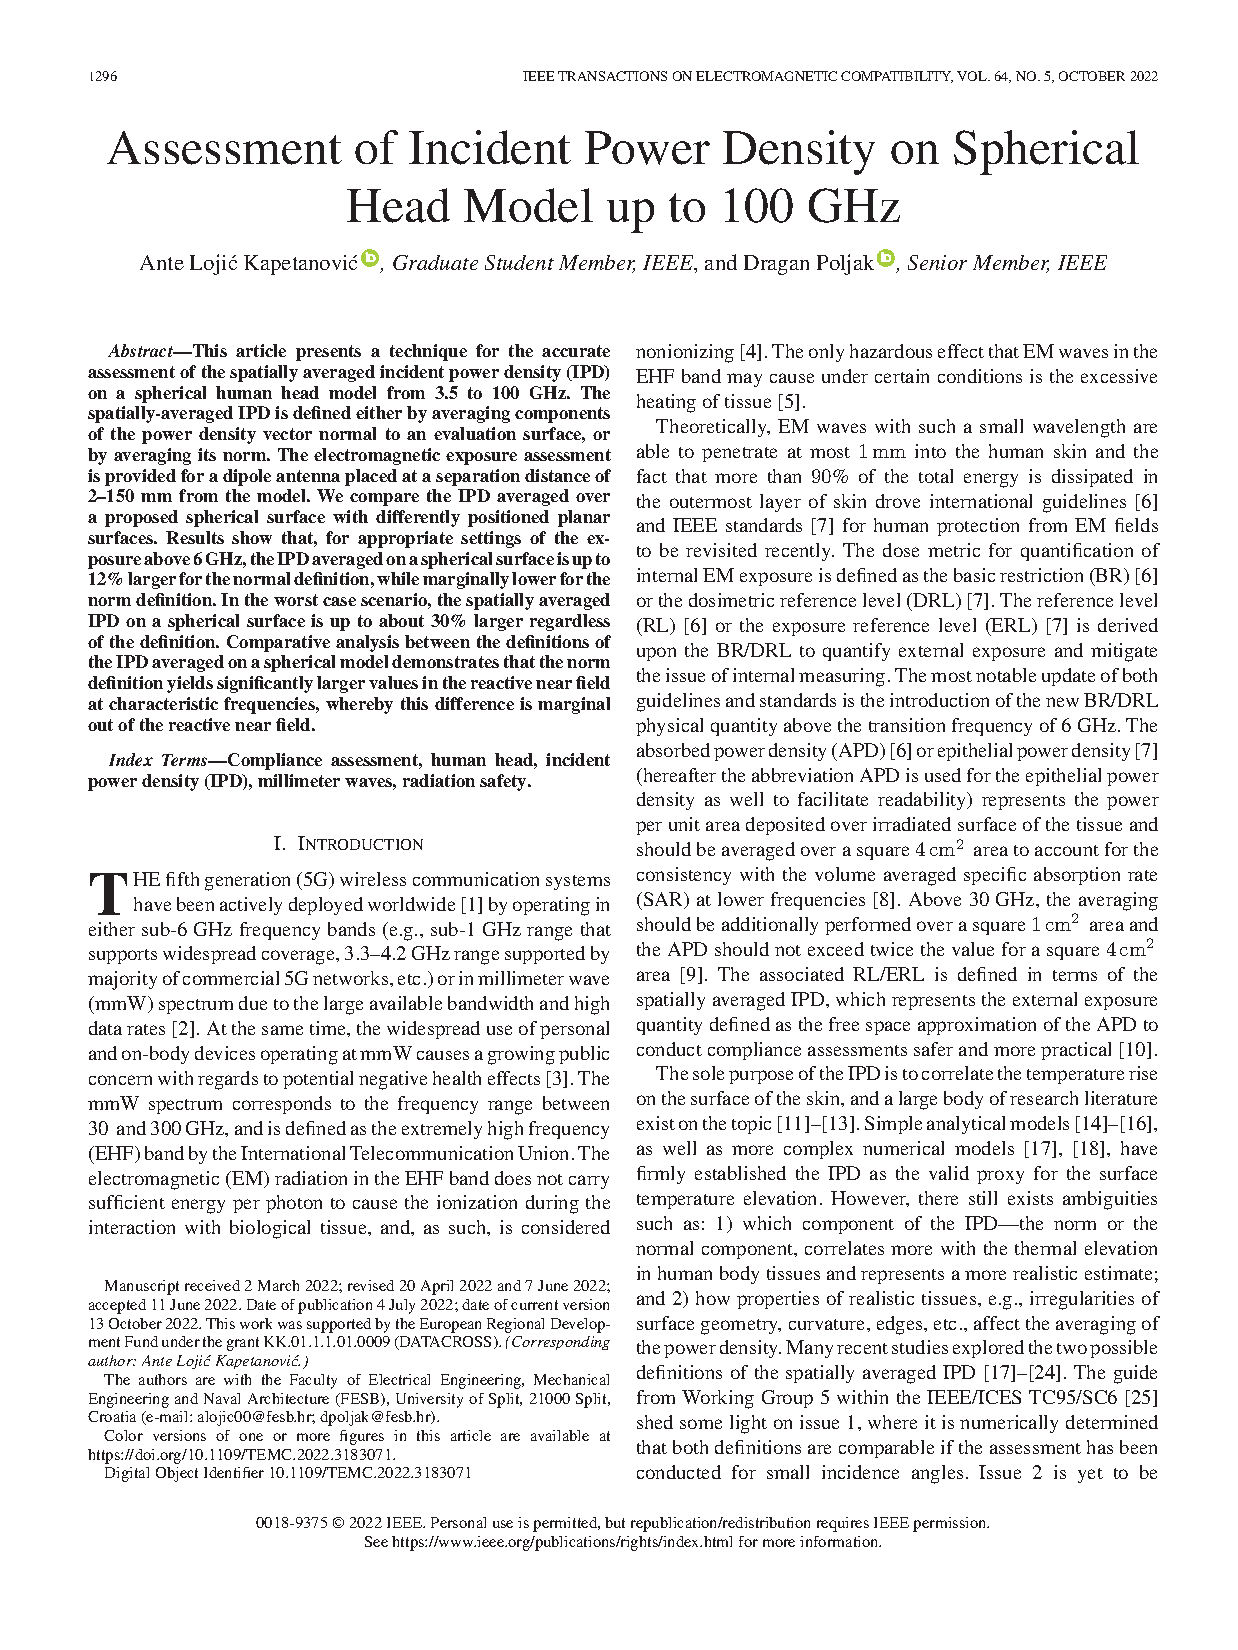
\includepdf[pages=-, pagecommand={\thispagestyle{includepdfstyle}}]{papers/Kapetanovic2022temc.pdf}

    \cleardoublepage

\chapter{}
\label{chap:b}

\begin{description}[leftmargin=!,labelwidth=\widthof{\bfseries Volume and number}]
    \item[Title] Machine learning-assisted antenna modelling for realistic assessment of incident power density on non-planar surfaces above 6 GHz
    \item[Authors] Ante Kapetanović, Dragan Poljak
    \item[Journal] Radiation Protection Dosimetry
    \item[Year] 2023
    \item[Volume and number] 199, 8--9
    \item[Pages] 826--834
    \item[Categorization] Research paper
    \item[Language] English
    \item[Abstract] In this paper, the analysis of exposure reference levels is performed for the case of a half-wavelength dipole antenna positioned in the immediate vicinity of non-planar body parts.
    The incident power density (IPD) spatially averaged over the spherical and cylindrical surface is computed at the 6–90 GHz range, and subsequently placed in the context of the current international guidelines and standards for limiting exposure to electromagnetic (EM) fields which are defined considering planar computational tissue models.
    As numerical errors are ubiquitous at such high frequencies, the spatial resolution of EM models needs to be increased which in turn results in increased computational complexity and memory requirements.
    To alleviate this issue, we hybridise machine learning and traditional scientific computing approaches through differentiable programming paradigm.
    Findings demonstrate a strong positive effect the curvature of non-planar models has on the spatially averaged IPD with up to 15\% larger values compared to the corresponding planar model in considered exposure scenarios.
    \item[Databases] Scopus, Google Scholar, Web of Science Core Collection -- Science Citation Index Expanded
    \item[Impact factor] 1.053
    \item[DOI] \href{https://doi.org/10.1093/rpd/ncad114}{\url{10.1093/rpd/ncad114}}
    \item[Copyright notice] \copyright 2023 Oxford University Press. Reprinted, with permission, from Ante Kapetanović and Dragan Poljak, Machine learning-assisted antenna modelling for realistic assessment of incident power density on non-planar surfaces above 6 GHz, Radiation Protection Dosimetry, 2023
\end{description}

\cleardoublepage

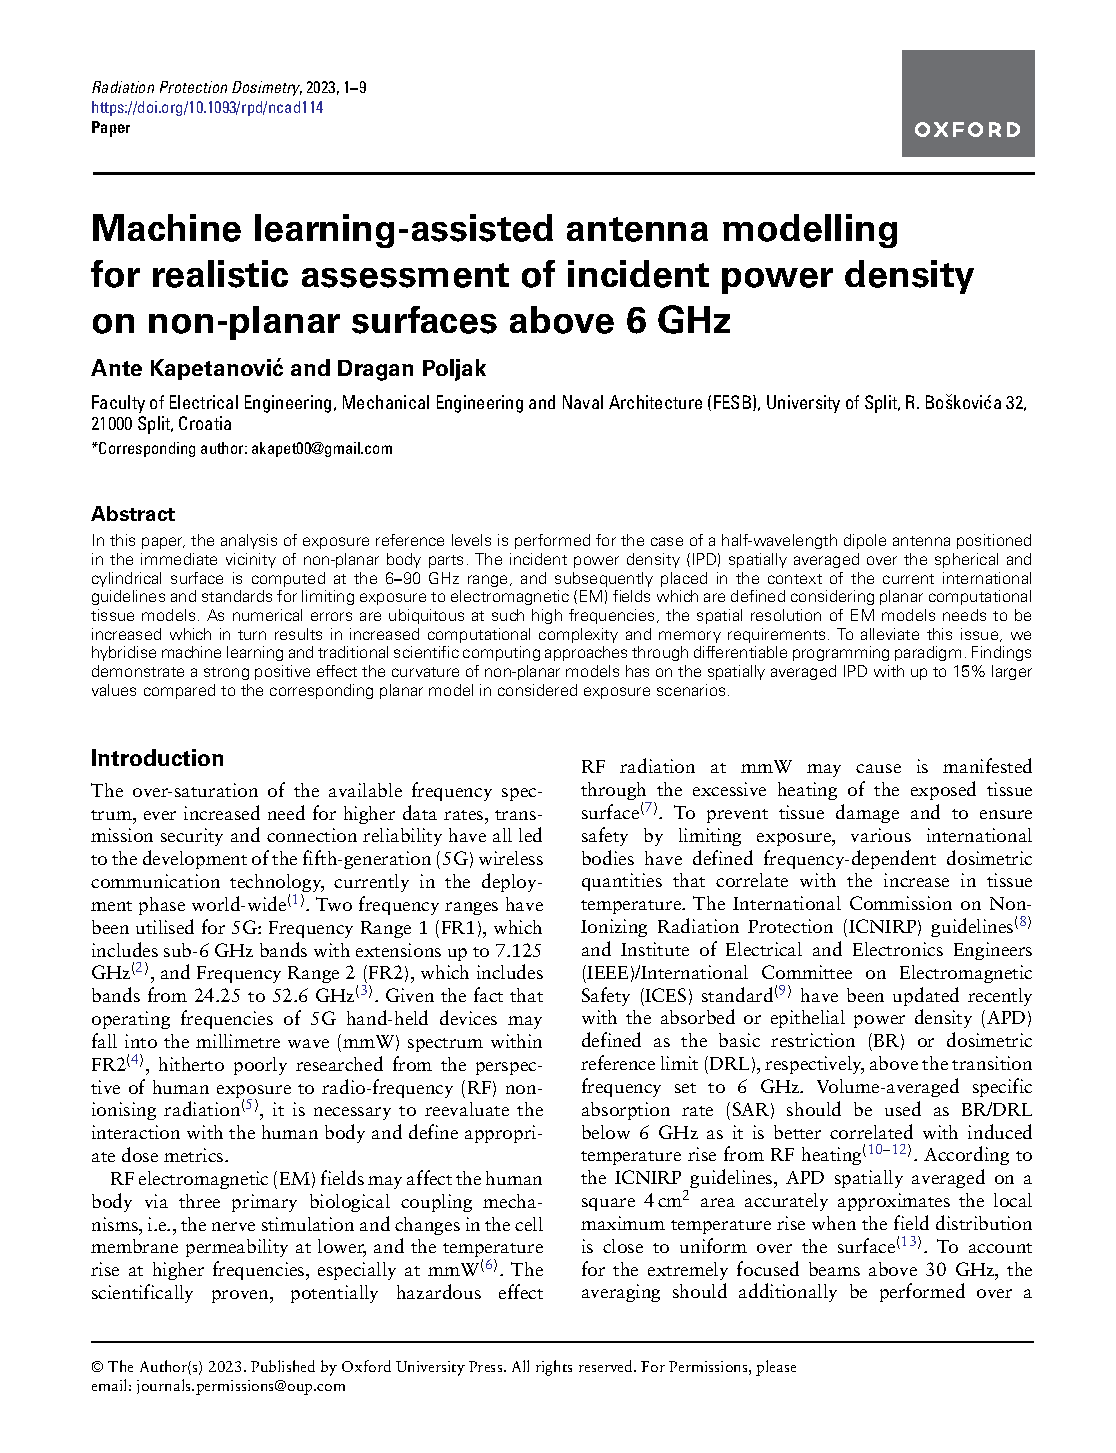
\includepdf[pages=-, pagecommand={\thispagestyle{includepdfstyle}}]{papers/Kapetanovic2023rpd.pdf}

    \cleardoublepage

\chapter{}
\label{chap:c}

\begin{description}[leftmargin=!,labelwidth=\widthof{\bfseries Volume and number}]
    \item[Title] Area-Averaged Transmitted and Absorbed Power Density on a Realistic Ear Model
    \item[Authors] Ante Kapetanović, Giulia Sacco, Dragan Poljak, Maxim Zhadobov
    \item[Journal] IEEE Journal of Electromagnetics, RF, and Microwaves in Medicine and Biology
    \item[Year] 2023
    \item[Volume and number] 7, 1
    \item[Pages] 39--45
    \item[Categorization] Research paper
    \item[Language] English
    \item[Keywords] Absorbed power density, electromagnetic dosimetry, millimeter waves, realistic ear model
    \item[Abstract] At millimeter waves (MMW), the current state of research in computational dosimetry is mainly relying on flat-surface tissue-equivalent models to simplify the exposure assessment by disregarding geometrical irregularities characteristic of conformal surfaces on realistic models.
    However, this can lead to errors in estimation of dosimetric quantities on non-planar body parts with local curvature radii comparable to the wavelength of the incident field.
    In this study, we address this problem by developing an averaging technique for the assessment of the absorbed power density ($S_\text{ab}$) on the anatomically-accurate electromagnetic (EM) model of the human ear.
    The dosimetric analysis is performed for the plane-wave exposure at 26 and 60 GHz, and the accuracy of the proposed method is verified by using two commercial EM software. Furthermore, we compare the two definitions of $S_\text{ab}$ provided in the international guidelines and standards for limiting exposure to EM fields above 6 GHz.
    Results show marginal relative differences between the obtained values from the two different definitions (within about 6\%) in all considered scenarios.
    On the other hand, in comparison to flat models, the spatial maximum $S_\text{ab}$ on the ear is up to about 20\% larger regardless of definition.
    These findings demonstrate a promising potential of the proposed method for the assessment of $S_\text{ab}$ on surfaces of anatomical models at frequencies upcoming for the 5th generation (5G) wireless networks and beyond.
    \item[Databases] Scopus, Google Scholar, Web of Science Core Collection -- Emerging Sources Citation Index
    \item[Impact factor] 3
    \item[DOI] \href{https://doi.org/10.1109/JERM.2022.3225380}{\url{10.1109/JERM.2022.3225380}}
    \item[Copyright notice] \copyright 2023 IEEE. Reprinted, with permission, from Ante Kapetanović, Giulia Sacco, Dragan Poljak and Maxim Zhadobov, Area-Averaged Transmitted and Absorbed Power Density on a Realistic Ear Model, IEEE Journal of Electromagnetics, RF, and Microwaves in Medicine and Biology, 2023
\end{description}

\cleardoublepage

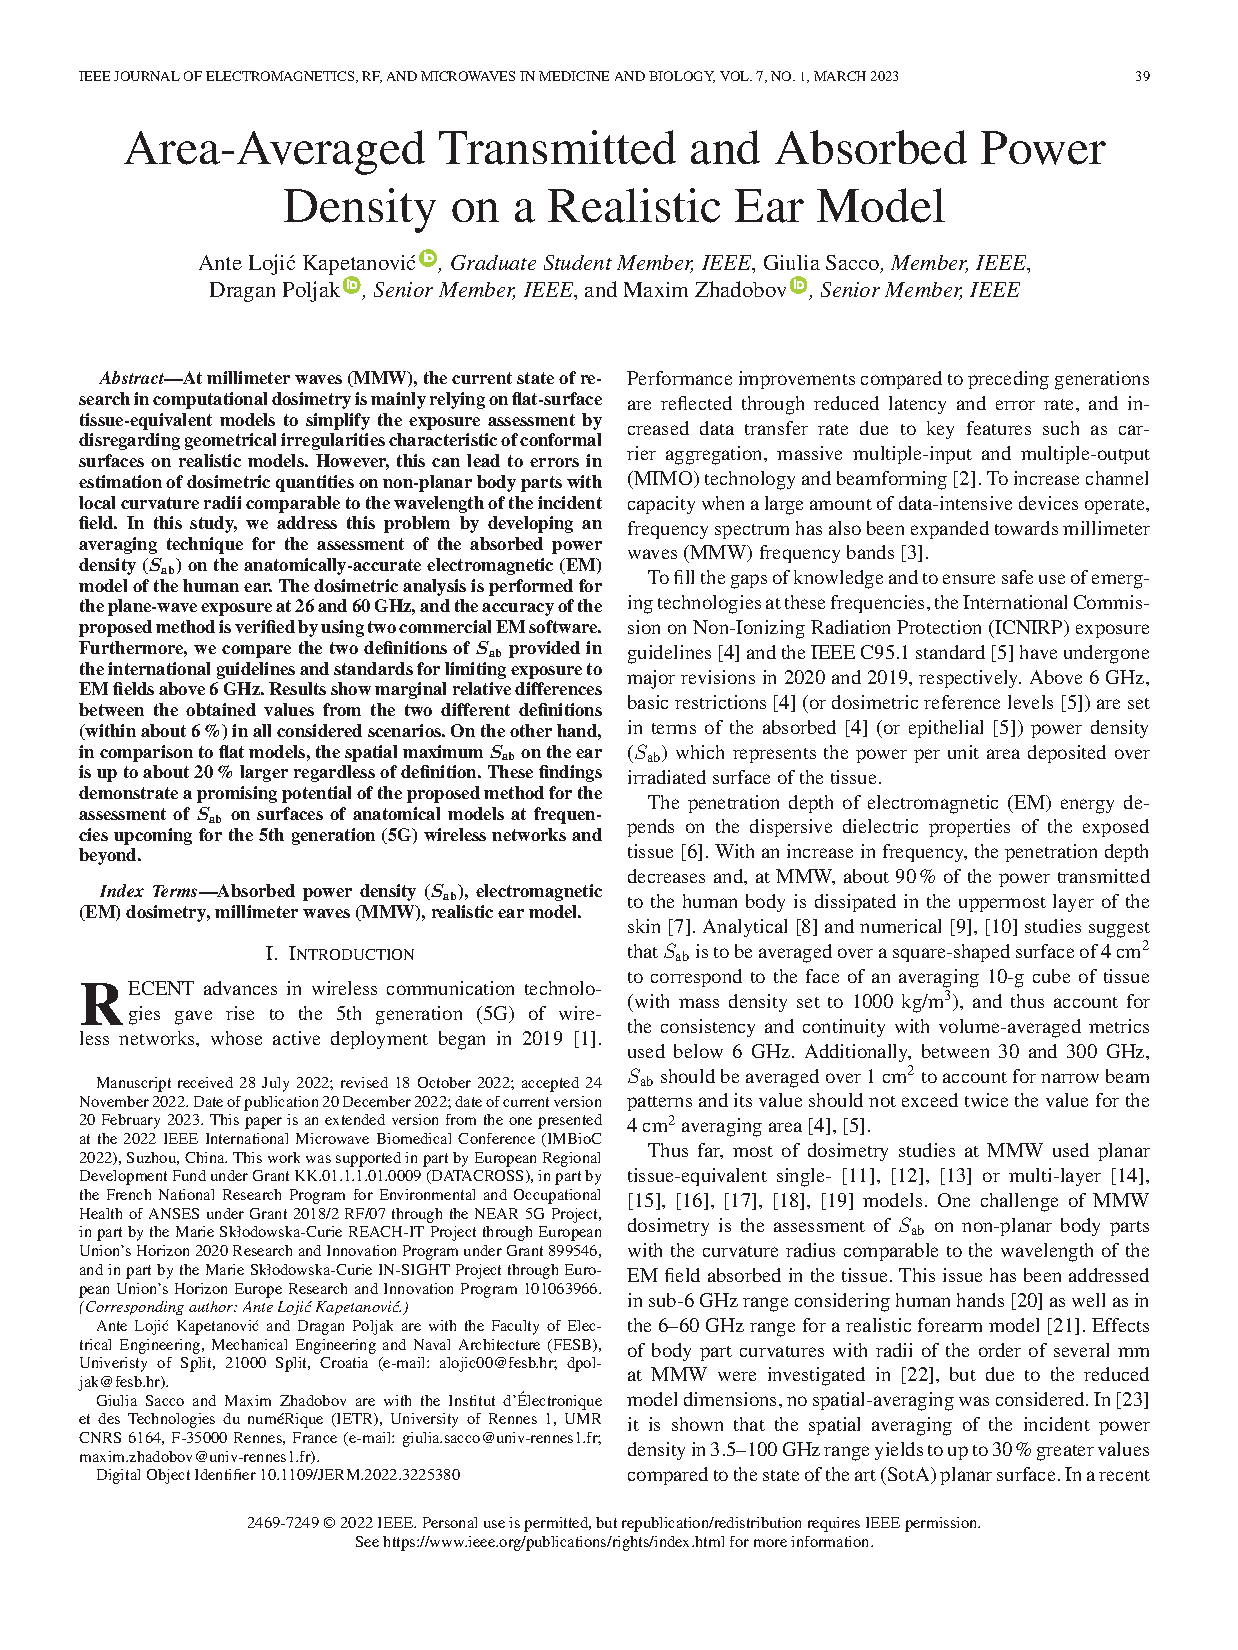
\includepdf[pages=-, pagecommand={\thispagestyle{includepdfstyle}}]{papers/Kapetanovic2023jerm.pdf}

    \cleardoublepage

\chapter{}
\label{chap:d}

\begin{description}[leftmargin=!,labelwidth=\widthof{\bfseries Volume and number}]
    \item[Title] On the Applicability of Numerical Quadrature for Double Surface Integrals at 5G Frequencies
    \item[Authors] Mario Cvetković, Dragan Poljak, Ante Kapetanović, Hrvoje Dodig
    \item[Journal] Journal of Communications Software and Systems
    \item[Year] 2022
    \item[Volume and number] 18, 1
    \item[Pages] 42--53
    \item[Categorization] Research paper
    \item[Language] English
    \item[Keywords] Dunavant rules, integral equation formulation, numerical integration, 5G frequencies, computational cost
    \item[Abstract] The human exposure assessment to wireless communications systems including the fifth generation (5G) mobile systems is related to determining the specific absorption rate (SAR) or the absorbed power density (APD).
    The assessment of both quantities requires the use of various numerical techniques, including moments method (MoM).
    As the use of MoM results in a fully populated system matrix, a tremendous computational cost is incurred, both in terms of matrix fill time and memory allocation, as the matrix size is directly related to frequency of the problem.
    This paper investigates the applicability of numerical integration at frequencies related to 5G.
    The novelty of this work is related to the comprehensive set of tests of various combination of source and observation triangles using the developed unit cube test.
    A number of convergence tests were performed to investigate the effects of the increasing frequency and the discretization scheme on the numerical solution, as well as to determine how to curb the computational requirements by the proficient use of numerical integration.
    The results show that in the lower gigahertz range, lower integration orders could be used, resulting in the decrease of matrix fill time without loss of solution accuracy.
    \item[Databases] Scopus, Google Scholar, Web of Science Core Collection -- Emerging Sources Citation Index
    \item[Impact factor] 0.6
    \item[DOI] \href{https://doi.org/10.24138/jcomss-2021-0183}{\url{10.24138/jcomss-2021-0183}}
    \item[Copyright notice] \copyright 2022 Croatian Communications and Information Society. Reprinted, with permission, from Mario Cvetković, Dragan Poljak, Ante Kapetanović, and Hrvoje Dodig, On the Applicability of Numerical Quadrature for Double Surface Integrals at 5G Frequencies, Journal of Communications Software and Systems, 2022
\end{description}

\cleardoublepage

\includepdf[scale=0.975, pages=-, pagecommand={\thispagestyle{includepdfstyle}}]{papers/Cvetkovic2022jcomss.pdf}

    \end{appendices}
    
    % CV
    \cleardoublepage
\pagestyle{empty}

\section*{Curriculum Vitae}
\vspace{15mm}
\noindent \textbf{Ante Kapetanović} was born in Split, Croatia, in 1995.
He graduated from the Grammar School for Natural Sciences and Mathematics in Split, Croatia and subsequently pursued his undergraduate degree in Electrical Engineering in 2014 at the Faculty of Electrical Engineering.
In 2017, he furthered his studies by enrolling in the graduate program for Electronics and Computer Engineering.
Ante successfully completed his M.S. degree in Electrical Engineering at the Faculty of Electrical Engineering, Mechanical Engineering, and Naval Architecture, University of Split, Split, Croatia, in 2019.
To date, he has been working toward the Ph.D. degree in computational bioelectromagnetics with the University of Split.

Ante did a three-month research visit at the Aalborg University, Aalborg, Denmark during his M.S.
Additionally, he participated in two short-term research visits at the IETR/CNRS in Rennes, France in 2021 and 2022.

His research interests revolve around human exposure to electromagnetic fields, computational bioelectromagnetics, numerical methods and techniques, physics-informed machine learning and scientific computing in general.
He has authored and co-authored six journal and more than fifteen conference papers in various fields of computational science.
His research was recognized at the 2022 IEEE MTT-S International Microwave Biomedical Conference in Sozhou, China, where he received the overall Best Student Paper Award.

Ante actively participates in professional societies and associations.
He has been a member of the Croatian Chapter of the IEEE Electromagnetic Compatibility Society since 2020 and a Student Member of the BioEM (previously European Bioelectromagnetics Association (EBEA) before a merger with The Bioelectromagnetics Society (BEMS)) since 2021.
Currently, he is an active member of IEEE Working Group on power density averaging methods within International Committee on Electromagnetic Safety (ICES), Technical Committee 95, Sub-Committee 6 on electromagnetic field dosimetry modeling.

\cleardoublepage
\pagestyle{empty}
\section*{Životopis}
\vspace{15mm}
\noindent
\textbf{Ante Kapetanović} rođen je u Splitu 1995. godine.
Po završetku srednjoškolskog obrazovanja kojeg je stekao u III. gimnaziji Split (Prirodoslovno-matematička gimnazija u Splitu, popularni MIOC), 2014. godine je upisao preddiplomski studij Elektrotehnike i informacijske tehnologije a 2017. godine i diplomski studij Elektronike i računalnog inženjerstva.
Titulu magistra inženjera elektrotehnike je stekao 2019. godine na Fakultetu elektrotehnike, strojarstva i brodogradnje pri Sveučilištu u Splitu.
Od kraja 2019. godine, zaposlen je kao mlađi istraživač u području računalnog bioelektromagnetizma na Sveučilištu u Splitu.

Ante je boravio tri mjeseca na istraživačkom posjetu na Sveučilištu Aalborg, Aalborg, Danska, tijekom diplomskog studija.
Tijekom doktorata, dva puta posjećuje institut IETR/CNRS, Rennes, Francuska, u sklopu suradnje na znanstvenim projektima.

Njegovi istraživački interesi su izloženost ljudi elektromagnetskim poljima, računalni bioelektromagnetizam, numeričke metode i tehnike, strojno učenje utemeljeno na fizici i znanstveno računanje općenito.
Do danas je autor i suator šest radova u časopisima i više od petnaest konferencijskih radova iz različitih područja računalnih znanosti.
Njegovo je istraživanje prepoznato na međunarodnoj konferenciji IEEE MTT-S u Sozhouu, Kina, gdje je 2022. godine dobio nagradu za najbolji studentski rad.

Ante je član hrvatskog ogranka IEEE društva za elektromagnetsku kompatibilnost od 2020. i student-član BioEM društva (prethodno Europske udruge za bioelektromagnetizam (EBEA) prije spajanja s Bioelektromagnetskim društvom (BEMS)) od 2021. godine.
Također je član i IEEE Radne skupine za metode određivanja gustoće snage, Tehničkog odbora 95 (Pododbor 6 za modeliranje dozimetrije elektromagnetskog polja), Međunarodnog odbora za elektromagnetsku sigurnost (ICES).
\newpage
}%
\end{document}